\documentclass[11pt,a4paper]{article}
\usepackage{acl}
\usepackage{arydshln}
\usepackage{booktabs}
\usepackage{times}
\usepackage{amssymb}
\usepackage{xcolor}
\usepackage{forest}
\usepackage{graphicx}
\usepackage{float}
\usepackage{tikz-qtree}
\usepackage{latexsym}
\usepackage{xspace}
\usepackage{algorithm}
\usepackage{algorithmicx}
\usepackage{inconsolata}
\usepackage[title]{appendix}
\renewcommand{\UrlFont}{\ttfamily\small}
\usepackage{enumitem,kantlipsum}
\usepackage{amsmath}

\newtheorem{problem}{Problem}
\usepackage{microtype}
\renewcommand{\baselinestretch}{0.969}

\def\aclpaperid{} %  Enter the acl Paper ID here

\setlength\titlebox{5cm}

% Our commands
\def\SPSB#1#2{\rlap{\textsuperscript{\textcolor{blue}{#1}}}\SB{#2}}
\def\SP#1{\textsuperscript{\textcolor{blue}{#1}}}
\def\SB#1{\textsubscript{\textcolor{blue}{#1}}}
\def\SBR#1{\textsubscript{\textcolor{red}{#1}}}

\newcommand\BibTeX{B\textsc{ib}\TeX}

\newcommand{\exa}[1]{``{#1}''}

\def\radius{0.4cm}
\newcommand{\bl}[1]{\textcolor{blue}{#1}}
\newcommand*\rot{\rotatebox{90}}
\newcommand{\pms}[1]{\footnotesize $\pm$#1}
\usepackage[position=b]{subcaption}
\usepackage{graphicx}
\usepackage{hyperref}
\usepackage{linguex}
\usepackage{tikz}
\usepackage{fixmetodonotes}

\title{The Paradox of the Compositionality of Natural Language: \\A Neural Machine Translation Case Study}

\author{Verna Dankers \\
  ILCC, University of Edinburgh \\
  \texttt{\small vernadankers@gmail.com} \\\And
  Elia Bruni \\
  University of Osnabr\"uck \\
  \texttt{\small elia.bruni@gmail.com} \\\And
  Dieuwke Hupkes \\
  Facebook AI Research \\
  \texttt{\small dieuwkehupkes@fb.com}}

\begin{document}
\maketitle

\begin{abstract}
As a popular paradigm for juggling data privacy and collaborative training, federated learning~(FL) is flourishing to distributively process the large scale of heterogeneous datasets on edged clients. Due to bandwidth limitations and security considerations, it ingeniously splits the original problem into multiple subproblems to be solved in parallel, which empowers \textit{primal dual} solutions to great application values in FL. In this paper, we review the recent development of classical \textit{federated primal dual} methods and point out a serious common defect of such methods in non-convex scenarios, which we say is a ``dual drift'' caused by dual hysteresis of those longstanding inactive clients under partial participation training. To further address this problem, we propose a novel \textit{\textbf{A}ligned \textbf{Fed}erated \textbf{P}rimal \textbf{D}ual}~(\textit{\textbf{A-FedPD}}) method, which constructs virtual dual updates to align global consensus and local dual variables for those protracted unparticipated local clients. Meanwhile, we provide a comprehensive analysis of the optimization and generalization efficiency for the \textit{A-FedPD} method on smooth non-convex objectives, which confirms its high efficiency and practicality. Extensive experiments are conducted on several classical FL setups to validate the effectiveness of our proposed method. 
\end{abstract}

%%%%%%%%%%%%%%%%%%%%%%%%%%%%%%%%%%%%%%%%%%%%%%%%%%
\section{Introduction}
\label{main:sec:introduction}
%%%%%%%%%%%%%%%%%%%%%%%%%%%%%%%%%%%%%%%%%%%%%%%%%%

\glsresetall

% \ljh{Just a draft. need polishing and proofreading}
A \gls{np}~\citep{garnelo2018conditional,garnelo2018neural} meta-learns a stochastic process describing the relationship between inputs and outputs in a given data stream, where each task in the data stream consists of a meta-training set of input-output pairs and also a meta-validation set. The \gls{np} then defines an implicit stochastic process whose functional form is determined by a neural network taking the meta-training set as an input, and the parameters of the neural network are optimized to maximize the predictive likelihood for the meta-validation set. This approach is philosophically different from the traditional learning pipeline where one would first elicit a stochastic process from the known class of models (e.g., \glspl{gp}) and hope that it describes the data well. An ideal \gls{np} would assume minimal inductive biases and learn as much as possible from the data. In this regard, \glspl{np} can be framed as a ``data-driven'' way of choosing proper stochastic processes.

 An important design choice for a \gls{np} model is how to capture the uncertainty in the random functions drawn from stochastic processes. When mapping the meta-training set into a function, one might employ a deterministic mapping as in \citet{garnelo2018conditional}. However, it is more natural to assume that there may be multiple plausible functions that might have generated the given data, and thus encode the functional (epistemic) uncertainty as a part of the \gls{np} model. \citet{garnelo2018neural} later proposed to map the meta-training set into a fixed dimensional \emph{global latent variable} with a Gaussian posterior approximation. While this improves upon the vanilla model without such a latent variable~\citep{le2018empirical}, expressing the functional uncertainty only through the Gaussian approximated latent variable has been reported to be a bottleneck~\citep{louizos2019functional}. To this end, \citet{lee2020bootstrapping} and \citet{lee2022neural} propose to apply bootstrap to the meta-training set to use the uncertainty arising from the population distribution as a source for the functional uncertainty.

In this paper, we take a rather different approach to define the functional uncertainty for \glspl{np}. Specifically, we utilize the martingale posterior distribution~\citep{fong2021martingale}, a recently developed alternative to conventional Bayesian inference. In the martingale posterior, instead of eliciting a likelihood-prior pair and inferring the Bayesian posterior, we elicit a joint predictive distribution on future data given observed data. Under suitable conditions on such a predictive distribution, it can be shown that the uncertainty due to the generated future data indeed corresponds to the uncertainty of the Bayesian posterior. Following this, we endow a \gls{np} with a joint predictive distribution defined through neural networks and derive the functional uncertainty as the uncertainty arising when mapping the randomly generated future data to the functions. Compared to the previous approaches of either explicitly positing a finite-dimensional variable encoding the functional uncertainty or deriving it from a population distribution, our method makes minimal assumptions about the predictive distribution and gives more freedom to the model to choose the proper form of uncertainty solely from the data. Due to the theory of martingale posteriors, our model guarantees the existence of the martingale posterior corresponding to the valid Bayesian posterior of an implicitly defined parameter. 
% \ed{Does the following make sense: }
Furthermore, working in the space of future observations allows us to incorporate the latent functional uncertainty path with deterministic path in a more natural manner.
% \ljh{It would be good to have more concrete motivation to prefer the martingale posteriors over conventional Bayesian inference; what would be an advantage of doing that, aside from the fact that we don't need to choose likelihood and prior?} \ed{I'll have a think about this, and will also do some proofreading. Because of the time difference and my job hours, timing might be a bit tricky tomorrow. When would be the best time for me to proofread?}

We name our extension of \glspl{np} with the joint predictive generative models as the \gls{mpnp}. Throughout the paper, we propose an efficient neural network architecture for the generative model that is easy to implement, flexible, and yet guarantees the existence of the martingale posterior. We also propose a training scheme to stably learn the parameters of \glspl{mpnp}. Using various synthetic and real-world regression tasks, we demonstrate that \gls{mpnp} significantly outperforms the previous \gls{np} variants in terms of predictive performance.





% \gls{npf}~\citep{garnelo2018conditional, garnelo2018neural} is a class of parametric models which defines stochastic processes over given data using neural networks.
% Unlike classical stochastic processes (e.g. \glspl{gp}), \gls{npf} learns to fit a proper stochastic processes from data under meta-learning framework.
% The deterministic version of \gls{npf}, \glspl{cnp}~\citep{garnelo2018conditional} deterministically map each dataset to a certain stochastic process which does not consider functional uncertainty.
% In order to compensate for this problem, \glspl{np}~\citep{garnelo2018neural} introduce a global latent variable which captures functional uncertainty.
% \citet{le2018empirical} empirically shows that considering functional uncertainty in \glspl{np} improves the diversity in function realizations and the predictive performance for data.

% Although \glspl{np} tries to capture functional uncertainty, there is some limitations for \glspl{np} to well capture uncertainty with a Gaussian latent variable.
% To overcome this problem, there are some prior works which applying advanced functional uncertainty modeling strategies~\citep{lee2020bootstrapping}\citep{lee2022neural} instead of a global latent variable.
% \gls{bnp}~\citep{lee2020bootstrapping} employs the residual bootstrapping strategy to make more robust uncertainty estimation even for the data-model mismatch situation. 
% However, \gls{bnp} requires a high computational cost compared to \gls{np} due to it's residual bootstrapping strategy.
% \gls{neubnp}~\citep{lee2022neural} employs the recent computationally efficient bootstrapping of the neural network called Neural Bootstrapper~\citep{shin2021neural}.
% However, \gls{neubnp} multiplies Dirichlet distributed random bootstrap weights to features of context dataset which disturbs model to well recovers the given dataset.

% This paper presents a novel extension of \gls{npf} which introduces functional uncertainty by changing posterior uncertainty on function parameters as predictive uncertainty on the unseen data conditional on the observed data...


\begin{table*}[!h]
\small
\centering
\resizebox{1.94\columnwidth}{!}{
\begin{subtable}[b]{\columnwidth}
\begin{tabular}{cll}
\toprule
\vspace{-0.5mm}
$n$ & \textbf{Template} \\ \midrule
1   & The \bl{N}\SPSB{}{people} \bl{V} the \bl{N}\SPSB{sl}{people} . \\
    %& \textit{The poet criticises the king .} \\
2   & The \bl{N}\SPSB{}{people} \bl{Adv} \bl{V} the \bl{N}\SPSB{sl}{people} . \\ 
    %& \textit{The victim carefully observes the queen .}\\
3   & The \bl{N}\SPSB{}{people} \bl{P} the \bl{N}\SPSB{sl}{vehicle} \bl{V} the \bl{N}\SPSB{sl}{people} . \\ 
    %& \textit{The athlete near the bike observes the leader .} \\
4   & The \bl{N}\SPSB{}{people} and the \bl{N}\SPSB{}{people} \bl{V} the \bl{N}\SPSB{sl}{people} . \\
    %& \textit{The poet and the child understand the mayor .} \\
5   & The \bl{N}\SPSB{sl}{quantity} of \bl{N}\SPSB{pl}{people} \bl{P} the \bl{N}\SPSB{sl}{vehicle} \bl{V} the \bl{N}\SPSB{sl}{people} . \\
    %& \textit{The group of men near the bike forgets the queen .} \\
6   & The \bl{N}\SPSB{}{people} \bl{V} that the \bl{N}\SPSB{pl}{people} \bl{V}. \\
    %& \textit{The farmer sees that the lawyers cry .} \\
7   & The \bl{N}\SPSB{}{people} \bl{Adv} \bl{V} that the \bl{N}\SPSB{pl}{people} \bl{V} . \\
    %& \textit{The mother probably thinks that the men scream .} \\
8   & The \bl{N}\SPSB{}{people} \bl{V} that the \bl{N}\SPSB{pl}{people} \bl{V} \bl{Adv} . \\
    %& \textit{The mother thinks that the men scream carefully .} \\
9   & The \bl{N}\SPSB{}{people} that \bl{V} \bl{V} the \bl{N}\SPSB{sl}{people} . \\
    %& \textit{The poets that sleep understand the queen .} \\
10  & The \bl{N}\SPSB{}{people} that \bl{V} \bl{Pro} \bl{V} the \bl{N}\SPSB{sl}{people} . \\
    %& \textit{The man that criticises him recognises the queen .} \\
    \bottomrule
    \end{tabular}
    \caption{Synthetic templates\vspace{-1.5mm}}
    \label{tab:synthetic_data}
\end{subtable}\begin{subtable}[b]{\columnwidth}
\small
\centering
\begin{tabular}{cll}
\toprule
\vspace{-0.5mm}
$n$ & \textbf{Template} \\ \midrule
1,2,3 & The \bl{N}\SPSB{}{people} \textcolor{red}{VP}\SBR{1,2,3} . \\
      & \textit{The men are gon na have to move off-camera .} \\
4,5   & The \bl{N}\SPSB{}{people} read(s) an article about \textcolor{red}{NP}\SBR{1,2} . \\ 
      & \textit{The man reads an article about the development} \\
      & \textit{of ascites in rats with liver cirrhosis .} \\
6,7   & An article about \textcolor{red}{NP}\SBR{3,4} is read by \bl{N}\SPSB{}{people} . \\ 
      & \textit{An article about the criterion on price stability ,} \\
      & \textit{which was 27 \% , is read by the child .} \\
8,9,10& Did the \bl{N}\SPSB{}{people} hear about \textcolor{red}{NP}\SBR{5,6,7} ? \\
      & \textit{Did the teacher hear about the march on} \\
      & \textit{Employment which happened here on Sunday ?} \\
    \bottomrule
    \end{tabular}
    \caption{Semi-natural templates\vspace{-1.5mm}}
    \label{tab:semi_natural}
\end{subtable}
}
\caption{The synthetic and semi-natural templates, with POS tags of the lexical items varied shown in blue with the plurality as superscript and the subcategory as subscript.  The OPUS-extracted NP and VP fragments are red.}
\vspace{-0.3cm}
\end{table*}




%%%%%%%%%%%%%%%%%%%%%%%%%%%%%%%%%%%%%%%%%%%%%%%%%%
\section{Background}
\label{main:sec:background}
%%%%%%%%%%%%%%%%%%%%%%%%%%%%%%%%%%%%%%%%%%%%%%%%%%
\subsection{Settings and notations}

Let $\calX = \bbR^{\din}$ be an input space and $\calY = \bbR^\dout$ be an output space. 
We are given a set of \emph{tasks} drawn from an (unknown) task distribution, $\tau_1, \tau_2, \dots \iidsim p_\text{task}(\tau)$. 
A task $\tau$ consists of a dataset $Z$ and an index set $c$, where $Z = \{z_i\}_{i=1}^n$ with each $z_i = (x_i, y_i) \in \calX \times \calY$ is a pair of an input and an output. We assume $Z$ are i.i.d. conditioned on some function $f$. The index set $c \subsetneq [n]$ where $[n] := \{1,\dots, n\}$ defines the \emph{context set} $Z_c = \{z_i\}_{i\in c}$. The \emph{target set} $Z_t$ is defined similarly with the index $t := [n]\setminus c$.

% Let $\calX = \bbR^{\din}$ be an input space and $\calY = \bbR^\dout$ be an output space. 
% We are given a set of \emph{tasks} drawn from an (unknown) task distribution, $\tau_1, \tau_2, \dots \iidsim p_\text{task}(\tau)$. 
% Each task $\tau$ consists of a tuple $\calD = (X, Y)$ and an index set $c \subsetneq [n]$ where $[n] := \{1,\dots, n\}$. Here, $X = \{x_i\}_{i=1}^n$ is an input set with $x_i \in \calX$ and $Y = \{y_i\}_{i=1}^n$ is an output set with $y_i \in \calY$. The \emph{context set} indexed by $c$ is then defined as $\calD_c = (X_c, Y_c)$ with $X_c = \{x_i\}_{i\in c}$ and $Y_c = \{y_i\}_{i\in c}$. The \emph{target} index set $t$ is defined as $t := [n] \setminus c$, and the corresponding target set $\calD_t$ is defined similarly.

%%%%%%%%%%%%%%%%%%%%%%%%%%%%%%%%%%%%%%%%%%%%%%%%%%
\subsection{Neural process families}

Our goal is to train a class of random functions $f: \calX \to \calY$ that can effectively describe the relationship between inputs and outputs included in a set of tasks. Viewing this as a meta-learning problem, for each task $\tau$, we can treat the context $Z_c$ as a meta-train set and target $Z_t$ as a meta-validation set. We wish to meta-learn a mapping from the context $Z_c$ to a random function $f$ that recovers the given context $Z_c$ (minimizing meta-training error) and predicts $Z_t$ well (minimizing meta-validation error). Instead of directly estimating the infinite-dimensional $f$, we learn a mapping from $Z_c$ to a predictive distribution for finite-dimensional observations,
\[
p(Y | X, Z_c) = \int \bigg[\prod_{i\in c} p(y_i | f, x_i) \prod_{i\in t} p(y_i | f, x_i)\bigg] p(f|Z_c) \dee f,
\]
where we are assuming the outputs $Y$ are independent given $f$ and $X$. We further restrict ourselves to simple heteroscedastic Gaussian measurement noises,
\[
p(y|f, x) = \calN(y | \mu_\theta(x), \sigma^2_\theta(x)I_{\dout}),
\]
where $\mu_\theta: \calX \to \calY$ and $\sigma_\theta^2: \calX \to \bbR_+$ map an input to a mean function value and corresponding variance, respectively. $\theta \in \bbR^{h}$ is a parameter indexing the function $f$, and thus the above predictive distribution can be written as
\[
p(Y | X, Z_c) = \int 
\bigg[\prod_{i\in [n]} \calN(y_i|\mu_\theta(x_i), \sigma_\theta^2(x_i) I_\dout)\bigg] p(\theta|Z_c) \dee \theta.
\]
A \gls{np} is a parametric model which constructs a mapping from $Z_c$ to $\theta$ as a neural network. The simplest version, \gls{cnp}~\citep{garnelo2018conditional}, assumes a deterministic mapping from $Z_c$ to $\theta$ as
\[
p(\theta|Z_c) = \delta_{r_c}(\theta), \quad r_c = f_\text{enc}(Z_c ; \phi_\text{enc}),
\]
where $\delta_{a}(x)$ is the Dirac delta function (which gives zero if $x\neq a$ and $\int\delta_a(x) \dee x=1$) and $f_\text{enc}$ is a \emph{permutation-invariant} neural network taking sets as inputs~\citep{zaheer2017deep}, parameterized by $\phi_\text{enc}$. Given a summary $\theta= r_c$ of a context $Z_c$, the \gls{cnp} models the mean and variance functions $(\mu, \sigma^2)$ as
\[
(\mu_\theta(x), \log \sigma_\theta(x)) = f_\text{dec}(x, r_c ; \phi_\text{dec}),
\]
where $f_\text{dec}$ is a feed-forward neural network parameterized by $\phi_\text{dec}$. Here the parameters $(\phi_\text{enc}, \phi_\text{dec})$ are optimized to maximize the expected predictive likelihood over tasks, $\bbE_{\tau}[\log p(Y|X, Z_c)]$.

Note that in the \gls{cnp}, the mapping from $Z_c$ to $\theta$ is deterministic, so it does not consider \emph{functional uncertainty} or epistemic (model) uncertainty. To resolve this, \citet{garnelo2018neural} proposed \gls{np} which learns a mapping from an arbitrary subset $Z' \subseteq Z$ to a variational posterior $q(\theta|Z')$ approximating $p(\theta|Z')$ under an implicitly defined prior $p(\theta)$: 
\[
(m_{Z'}, \log s_{Z'}) = f_\text{enc}(Z'; \phi_\text{enc}), \quad p(\theta|Z') \approx q(\theta|Z') := \calN(\theta | m_{Z'}, s^2_{Z'}I_h).
\]
With $f_\text{enc}$, the \gls{elbo} for the predictive likelihood is written as
\[
\log p(Y|X,Z_c) &\geq \sum_{i\in[n]} \bbE_{q(\theta|Z)}[\log \calN(y_i|\mu_\theta(x_i), \sigma_\theta^2(x_i)I_\dout)] - \KL[q(\theta|Z)\Vert p(\theta|Z_c)] \nonumber\\
&\approx
\sum_{i\in[n]} \bbE_{q(\theta|Z)}[\log \calN(y_i|\mu_\theta(x_i), \sigma_\theta^2(x_i)I_\dout)] - \KL[q(\theta|Z)\Vert q(\theta|Z_c)].
\]
An apparent limitation of the \gls{np} is that it assumes a uni-modal Gaussian distribution as an approximate posterior for $q(\theta|Z_c)$. Aside from the limited flexibility, it does not fit the motivation of \glspl{np} trying to learn as much as possible in a data-driven manner, as pre-specified parametric families are used.  

There have been several improvements over the vanilla \glspl{cnp} and \glspl{np}, either by introducing attention mechanism~\citep{vaswani2017attention} for $f_\text{enc}$ and $f_\text{dec}$~\citep{kim2018attentive}, or using advanced functional uncertainty modeling~(\citealp{lee2020bootstrapping}; \citealp{lee2022neural}). We provide a detailed review of the architectures for such variants in \cref{app:sec:architectures}. Throughout the paper, we will refer to this class of models as \gls{npf}.

% \subsection{Neural Process Family}
% Consider a target dataset $\calD=(X,Y)$ where $X=\{x_i\}_{i=1}^n$ is an input set and $Y=\{y_i\}_{i=1}^n$ is an output set. 
% Here we define subset $\calD_C=(X_C,Y_C)=\{(x_i,y_i)\}_{i\in C}$ as our context dataset where $C\subsetneq [n]$ denotes an index set.
% With these $\calD$ and $\calD_C$, \gls{npf}\citep{garnelo2018conditional, garnelo2018neural} learns to make a stochastic process which maps $x\in X$ to some conditional distribution $p(y|x,X_C,Y_C)$ by maximizing
% \begin{align}
%     \log p(Y|X,\calD_C) = \sum_{i=1}^n \log p(y_i|x_i, \calD_C)=\sum_{i=1}^n \log p(y_i|x_i,X_C,Y_C).
% \end{align}
% The deterministic \gls{npf} called \glspl{cnp}~\citep{garnelo2018conditional, gordon2020convolutional} predicts $p(y_i|x_i, X_C,Y_C)$ only with deterministic path which is made up with an \textit{permutation invariant}~\citep{zaheer2017deep} encoder neural network $f_{\enc}$ and a decoder neural network $f_{\dec}$.
% Here an encoder neural network $f_{\enc}$ compresses $(X_C,Y_C)$ into a feature $r_C$.
% A decoder neural network $f_{\dec}$ takes $r_C$ and $x_i$ as inputs and outputs the parameters of the distribution $p(y_i|x_i,X_C,Y_C)$.
% The conditional distribution $p(y_i|x_i,X_C,Y_C)$ is usually modelled as a Gaussian distribution.
% We can simplify these procedures as:
% \begin{align}
%     r_C = f_\enc(X_C,Y_C), \quad (\mu_i, \log\sigma_i)=f_\dec(x_i,r_C),\quad  p(y_i|x_i,X_C,Y_C)=\calN(y_i|\mu_i,\sigma_i^2).
% \end{align}

% The stochastic \gls{npf} called \glspl{np}~\citep{garnelo2018neural,foong2020meta} contains a latent path in addition to deterministic path to predict $p(y_i|x_i, X_C,Y_C)$.
% This latent path has an own permutation invariant latent encoder neural network $f_{\lat}$ and shares a decoder neural network $f_{\dec}$.
% $f_\lat$ takes $(X_C,Y_C)$ as an input and outputs the parameters of Gaussian distribution $p(z|X_C,Y_C)$ where $z$ is a global latent variable of \gls{np}.
% Global latent variable $z$ models a \textit{functional uncertainty} of \gls{np} which means that it helps \gls{np} to make the diverse conditional distribution $p(y_i|x_i,X_C,Y_C)$. With this latent path, the procedure of \glspl{np} can be summarized as:
% \begin{align}
%     &r_C = f_\enc(X_C,Y_C), \quad (\mu_z,\log\sigma_z)=f_\lat(X_C,Y_C),\quad z|\calD_C\sim\calN(\mu_z, \sigma_z^2)\\
%     &(\mu_i, \log\sigma_i)=f_\dec(x_i,r_C,z),\quad  p(y_i|x_i,X_C,Y_C)=\calN(y_i|\mu_i,\sigma_i^2).
% \end{align}
% In order to train \gls{np}, we can use ELBO of the conditional probability which is 
% \begin{align}
%     \log p(Y|X,\calD_C) \geq \sum_{i=1}^n \bbE_{q(z|\calD)}\left[\log p(y_i|x_i,z,r_C)\right]-\text{KL}(q(z|\calD)||p(z|\calD_C)).
% \end{align}
% If we approximate $p(z|\calD_C)$ by $q(z|\calD_C)$, this ELBO changes into our train loss function
% \begin{align}
%     \sum_{i=1}^n \bbE_{q(z|\calD)}\left[\log p(y_i|x_i,z,r_C)\right]-\text{KL}(q(z|\calD)||p(z|\calD_C)).
% \end{align}

%%%%%%%%%%%%%%%%%%%%%%%%%%%%%%%%%%%%%%%%%%%%%%%%%%
\subsection{Martingale Posterior Distributions}

The martingale posterior distribution \citep{fong2021martingale} is a recent generalization of Bayesian inference which reframes posterior uncertainty on parameters as {predictive} uncertainty on the unseen population conditional on the observed data. Given observed samples $Z = \{z_i\}_{i=1}^n$  i.i.d. from the sampling density $p_0$, one can define the parameter of interest as a functional of $p_0$, that is
$$
\theta_0 = \theta(p_0) =  \argmin_\theta\int \ell(z,\theta)\, p_0(dz), 
$$
where $\ell$ is a loss function. For example, $\ell(z,\theta) =  (z-\theta)^2$ would return $\theta_0$ as the mean, and $\ell(z,\theta)= - \log p(z \mid \theta)$ would return the KL minimizing parameter between $p(\cdot \mid \theta)$ and $p_0$.

The next step of the martingale posterior is to construct a \emph{joint} predictive density on $Z' = \{z_i\}_{i=n+1}^N$ for some large $N$, which we write as $p(Z' \mid Z)$. In a similar fashion to a bootstrap, one can imagine drawing $Z' \sim p(Z' \mid Z)$, then computing $\theta(g_N)$ where $g_N(z) = \frac{1}{N} \sum_{i=1}^N \delta_{z_i} (z)$. %\ljh{Define $\theta(g_N)$ somewhere?} 
The predictive uncertainty in $Z'$ induces uncertainty in $\theta(g_N)$ conditional on $Z$. The key connection is that  if $p(Z' \mid Z)$ is the Bayesian joint  posterior predictive density, and $\ell = - \log p(z \mid \theta)$, then $\theta(g_N)$ is distributed according to the Bayesian posterior $\pi(\theta \mid Z)$ as $N \to \infty$, under weak conditions. In other words, posterior uncertainty in $\theta$ is equivalent to predictive uncertainty in $\{z_i\}_{i=n+1}^\infty$. 

\cite{fong2021martingale} specify more general  $p(Z' \mid Z)$ directly beyond the Bayesian posterior predictive, and define the (finite) martingale posterior 
as 
$\pi_N(\theta \in A \mid Z) = \int \mathbbm{1}(\theta(g_N) \in A) \, p(dZ' \mid Z)$. In particular, the joint predictive density can be factorized into a sequence of 1-step-ahead predictives, 
$
p(Z' \mid Z) = \prod_{i=n+1}^N p(z_i \mid z_{1:i-1}),
$
and the sequence $\{p(z_i \mid z_{1:i-1})\}_{n+1}^N$ is elicited directly, removing the need for the likelihood and prior. Hyperparameters for the sequence of predictive distributions can be fitted in a data-driven way by maximizing 
$$\log p(Z) = \sum_{i=1}^n \log p(z_i \mid z_{1:i-1}),$$ 
which is analogous to the log marginal likelihood.  \cite{fong2021martingale} requires the sequence of predictives to be \gls{cid}, which is a martingale condition on the sequence of predictives that ensures $g_N$ exists almost surely. The Bayesian posterior predictive density is a special case, as exchangeability of $p(Z' \mid Z)$ implies the sequence of predictives is \gls{cid} In fact, De Finetti's theorem \citep{de1937prevision} guarantees that any exchangeable joint density implies an underlying likelihood-prior form, but specifying the predictive density directly can be advantageous. It allows for  easier computation, as we no longer require posterior approximations, and it also widens the class of available nonparametric predictives which we will see shortly.  

% \ljh{Will you describe what a ``martingale posterior'' actually is here? (Definition 1 in \citet{fong2021martingale})}.

% \ed{Just brainstorming some ideas below}

%  In the meta-learning context, for each $\tau_j \sim p(\tau)$, we are interested in  obtaining predictives $p_\phi( \mathcal{D}_c' \mid \mathcal{D}_c)$, where $\mathcal{D}_c' = \{z_i\}_{i = n+1:N}$ and $\mathcal{D}_c \mid \tau_j$ consists of i.i.d. samples. The log marginal likelihood for each task is $\log p(\mathcal{D}_c)$, so a valid training objective could be $E_\tau[\log p(\mathcal{D}_c)]$. However, as we specify $p(\mathcal{D}_c' \mid \mathcal{D}_c)$ directly, it is not obvious how to compute $\log p(\mathcal{D}_c)$. Instead, we could estimate this with  cross-validation, that is $p(\mathcal{D}_c^{\text{test}}\mid \mathcal{D}_c^{\text{train}})$, where $\mathcal{D}_c = \mathcal{D}_c^{\text{test}}\cup \mathcal{D}_c^{\text{train}}$. Or is there anything stopping us from using $p(\mathcal{D}_t \mid \mathcal{D}_c)$?
%  \ed{I was thinking $p(\calD_t|\calD_c)$ where $p$ is the generative model (not decoder), but I think this is very similar to $p(\mathcal{D}_c^{\text{test}}\mid \mathcal{D}_c^{\text{train}})$.}
%  \lhg{Ah... I see... Actually, I think we can't measure $p(\calD_t|\calD_c)$ without decoder. I also tried $p(\calD_c^{\text{test}}|\calD_c^{train})$ with decoder. }
%  \ed{Ah I see, because we only have a generative model right? That's a great motivator for the third term in (14) then. }
%  \lhg{yes. That's right:)}
%  {\textcolor{red}{Hyungi: I think we can try $p(\mathcal{D}_c^{\text{test}}\mid \mathcal{D}_c^{\text{train}})$ as our training objective and a minor curious point is "Is this training objective helps our generator to make some reasonable pseudo context data?". I think we have to check this with experiment. By the way $p(D_C''|D_C \cup (D_C'\textbackslash D_C''))$ loss did not work for directly generating pseudo context data framework.} }
 
%  \ed{{Maybe it makes sense that the old objective doesn't work too well, since $\mathcal{D}_C' $ is simulated from $p(\mathcal{D}_C' \mid \mathcal{D}_C)$, so it will always have high likelihood. Whereas checking the model on the actual observed $\mathcal{D}_c$ will force it to fit well?}}
 
%  \ed{Thanks for the update! By our feature model, do you mean the current objective in equation (14) performs the best? If so, maybe we should just stick to that then. We can also argue that it is somewhat difficult to estimate the density values $p(\mathcal{D}_C' \mid \mathcal{D}_C)$ as the predictive is generative, and the third term is kind of a proxy for this `marginal likelihood'. }
 
%  \lhg{Yeah, equation (14) performs the best. We are now doing some last trials on directly sampling version. As you said, I think we should stick to equation (14) and feature generating model.}
%  \ed{Nice, I think it's clear now and yes I agree :) I'll perhaps add a sentence after (14) to describe the lack of a tractable marginal likelihood density. Will comment out the above after.}
%  \lhg{That will be great for us. Thank you}
 
%  {\color{red} Edwin: Expand to meta-learning framework, may need discussion of amortization? Or leave in Section 3.1? }
%  {\color{red} Juho: I will discuss the amortization part in section 3.1.}

%%%%%%%%%%%%%%%%%%%%%%%%%%%%%%%%%%%%%%%%%%%%%%%%%%
\subsection{Exchangeable Generative Models}\label{main:subsec:exchangeable}

To construct a martingale posterior, we can either specify a sequence of one-step predictive distributions or the joint predictive density distribution directly, as long as the \gls{cid} condition is satisfied.  Here, we opt to specify an exchangeable $p(Z' \mid Z)$ directly, which then implies the required \gls{cid} predictives. We now briefly review exchangeable generative models which can be used to specify the exchangeable joint predictive.  For a set of random variables $Z = \{z_i\}_{i=1}^n$ with each $z_i\in \calZ = \bbR^{d}$, we say the joint distribution $p(Z)$ is \emph{exchangeable} if it is invariant to the arbitrary permutation of the indices, that is, $p(Z) = p(\pi\cdot Z)$ for any permutation $\pi$ of $[n]$. A simple way to construct such exchangeable random variables is to use a \emph{permutation-equivariant mapping}. A mapping $\bof: \calZ^n\to\calZ^n$ is permutation equivariant if $\bof(\pi\cdot Z) = \pi\cdot\bof(Z)$ for any $\pi$. Given $\bof$, we can first generate i.i.d. random variables and apply $\bof$ to construct a potentially correlated but exchangeable set of random variables $Z$ as follows:
\[
\calE := \{\varepsilon_i\}_{i=1}^n \iidsim p_0, \quad Z = \bof(\calE).
\]
For $\bof$, we employ the modules introduced in \citet{lee2019set}. Specifically, we use a permutation equivariant module called  \gls{isab}. An \gls{isab} mixes input sets through a learnable set of parameters called \emph{inducing points} via \glspl{mab}~\citep{vaswani2017attention,lee2019set}. 
\[
\textsc{isab}(\calE) = \textsc{mab}(\calE, H) \in \bbR^{n\times d}\text{ where } H = \textsc{mab}(I, \calE)\in \bbR^{m\times d}.
\]
Here, $I \in \bbR^{m\times d}$ is a set of $m$ inducing points and $\textsc{mab}(\cdot,\cdot)$ computes attention between two sets.
The time-complexity of an \gls{isab} is $O(nm)$, scales linear with input set sizes.

% \paragraph{Exchangeability}


% In order to generate a set structured data, model should satisfy a condition called \textit{exchangeability}~\citep{kim2021setvae}. Exchangeability condition means that the probability of generated set data does not depend on its ordering. To achieve exchangeability, a joint distribution of the generated set data should satisfy permutation invariance. In other words, for a set of random variables $\bX=\{X_i\}_{i=1}^n$ and for any permutation $\pi$, joint probability $p$ should satisfy:
% \begin{align}
%     p(\bX) = p(\pi(\bX)).
% \end{align}
% A nice and easy way to make a permutation invariant joint distribution is using a permutation equivariant function $f_{\text{per}}$ and \textit{i.i.d.} random variable set $\bX'=\{X_i'\}_{i=1}^n$ which is called \textit{permutation-equivariant generative framework}~\citep{kim2021setvae}.
% In this framework, if we let $\bX = f_{\text{per}}(\bX')$ then the joint distribution of $\bX$ satisfies permutation invariant.
% \paragraph{Set Transformer} Set Transformer~\citep{lee2019set} is an attention-based neural network model which satisfies permutation invariant property for input dataset. It contains permutation equivariant module called ISAB. ISAB transforms the input dataset $\bx\in\bbR^{n\times d}$ by a smaller set $I\in\bbR^{m\times d}$ called inducing points:
% \begin{align}
%     \text{ISAB}(\bx) &= \text{MAB}(\bx, \bH)\in\bbR^{n\times d},\\
%     \text{where } \bH &=\text{MAB}(I,\bx)\in\bbR^{m\times d}
% \end{align}
% where MAB is a Multihead Attention Block which is a part of the Transformer~\citep{vaswani2017attention} encoder block except dropout and positional encoding.


\section{Setup}

\section{Proposed model: \approach}
\label{pm}
In this paper we present an adaptive anomaly detection model for fixing leaf depths according to labels received from domain experts.
The core idea of the proposed approach is presented in Algorithm \ref{alg_albif} and relies on developing an Isolation Forest based model in which the detector has the possibility to query domain experts for labels. In this iterative environment, once the Isolation Forest is fully grown, the algorithm can choose the points to be labeled and, based on the novel information achieved, its core structure is modified, in order to obtain a strong increase in the performance, with the use of only a limited number of labeled points. For every iteration, such modification only takes place in the external node containing the queried point, maintaining the main structure of the Isolation Forest untouched. In this way, the main goal is, given the novel information, to update the Isolation Forest structure, readjusting it based on the labeled points.  

%% ALGORITHM STYLE -- Released 8 April 1996
%    for LaTeX-2e
% Copyright -- 1994 Peter Williams
% E-mail Peter.Williams@dsto.defence.gov.au
\NeedsTeXFormat{LaTeX2e}
\ProvidesPackage{algorithm}
\typeout{Document Style `algorithm' - floating environment}

\RequirePackage{float}
\RequirePackage{ifthen}
\newcommand{\ALG@within}{nothing}
\newboolean{ALG@within}
\setboolean{ALG@within}{false}
\newcommand{\ALG@floatstyle}{ruled}
\newcommand{\ALG@name}{Algorithm}
\newcommand{\listalgorithmname}{List of \ALG@name s}

% Declare Options
% first appearance
\DeclareOption{plain}{
  \renewcommand{\ALG@floatstyle}{plain}
}
\DeclareOption{ruled}{
  \renewcommand{\ALG@floatstyle}{ruled}
}
\DeclareOption{boxed}{
  \renewcommand{\ALG@floatstyle}{boxed}
}
% then numbering convention
\DeclareOption{part}{
  \renewcommand{\ALG@within}{part}
  \setboolean{ALG@within}{true}
}
\DeclareOption{chapter}{
  \renewcommand{\ALG@within}{chapter}
  \setboolean{ALG@within}{true}
}
\DeclareOption{section}{
  \renewcommand{\ALG@within}{section}
  \setboolean{ALG@within}{true}
}
\DeclareOption{subsection}{
  \renewcommand{\ALG@within}{subsection}
  \setboolean{ALG@within}{true}
}
\DeclareOption{subsubsection}{
  \renewcommand{\ALG@within}{subsubsection}
  \setboolean{ALG@within}{true}
}
\DeclareOption{nothing}{
  \renewcommand{\ALG@within}{nothing}
  \setboolean{ALG@within}{true}
}
\DeclareOption*{\edef\ALG@name{\CurrentOption}}

% ALGORITHM
%
\ProcessOptions
\floatstyle{\ALG@floatstyle}
\ifthenelse{\boolean{ALG@within}}{
  \ifthenelse{\equal{\ALG@within}{part}}
     {\newfloat{algorithm}{htbp}{loa}[part]}{}
  \ifthenelse{\equal{\ALG@within}{chapter}}
     {\newfloat{algorithm}{htbp}{loa}[chapter]}{}
  \ifthenelse{\equal{\ALG@within}{section}}
     {\newfloat{algorithm}{htbp}{loa}[section]}{}
  \ifthenelse{\equal{\ALG@within}{subsection}}
     {\newfloat{algorithm}{htbp}{loa}[subsection]}{}
  \ifthenelse{\equal{\ALG@within}{subsubsection}}
     {\newfloat{algorithm}{htbp}{loa}[subsubsection]}{}
  \ifthenelse{\equal{\ALG@within}{nothing}}
     {\newfloat{algorithm}{htbp}{loa}}{}
}{
  \newfloat{algorithm}{htbp}{loa}
}
\floatname{algorithm}{\ALG@name}

%\newcommand{\listofalgorithms}{\listof{algorithm}{\listalgorithmname}}



\begin{algorithm}
\caption{\textit{\approach$((x^{\mathcal{s}},y^{\mathcal{s}}), X^{\mathcal{u}}, F)$}}\label{alg_albif}
\KwData{labeled point $(x^{\mathcal{s}},y^{\mathcal{s}})$, unlabeled dataset $X^{\mathcal{u}}$, forest $F$}
\KwResult{updated forest $F$, query point $x^{\mathcal{s}}$} 
 $F \gets$ \textit{LeafDepthUpdate}$((x^{\mathcal{s}},y^{\mathcal{s}})$, $F)$\;
     $H \gets$ \textit{GetDepthMatrix}$(X^{\mathcal{u}}$, $F)$\;
    $x^{\mathcal{s}} \gets$ \textit{GetQuery}$(H)$

\end{algorithm}

\begin{algorithm}
\caption{\textit{LeafDepthUpdate$((x^{\mathcal{s}},y^{\mathcal{s}})$, $F)$}}\label{alg_leafDepth}
\KwData{labeled point $(x^{\mathcal{s}},y^{\mathcal{s}})$, unlabeled dataset $X^{\mathcal{u}}$, forest $F$}
\KwResult{updated leaf $L$} 
\For{$T_t$ \text{in} $F$}{
        $L \gets \lambda_{T_t}(x^{\mathcal{s}})$ \;
        \If{$y_{\mathcal{s}}==$ \text{anomaly}}{$L_\mathcal{o} \gets L_\mathcal{o} + 1$ \;}
        \Else{$L_\mathcal{i} \gets L_\mathcal{i} + 1$ \;}
        $L_\mathcal{h} \gets  h^\mathcal{s}(k(L))$
}
\end{algorithm}


\begin{algorithm}
\caption{\textit{GetDepthMatrix$(X^{\mathcal{u}}, F)$}}\label{alg_DepthMatrix}
\KwData{unlabeled dataset $X^{\mathcal{u}}$, forest $F$}
\KwResult{updated leaf $L$} 
\For{$T_t$ \text{in} $F$}{
    \For{$x^{\mathcal{u}}_j$ \text{in} $X^{\mathcal{u}}$}{
            $L \gets \lambda_{T_t}(x^{\mathcal{u}}_j)$ \;
            $H_{jt} \gets  h^\mathcal{s}(k(L))$
    }
}
\end{algorithm}


Specifically, the proposed approach may be outlined as follows. Let $X=\{x^1,\dots, x^n\}$ be a generic training dataset, where $x^i \in \mathbb{R}^m$, $i=1,\dots,n$. First, the Isolation Forest algorithm is trained, leading to a forest $F=\{T_t\}_{t=1}^{n_T}$ of fixed number $n_T$ of fully grown iTrees. By construction, $T=\{L_l\}_{l=1}^{n_L}$ namely each tree $T$ is characterized by a variable number of leaves $L$. We use the following form to describe each leaf $L$:
$L=(L_\mathcal{p}, L_H, L_\mathcal{i}, L_\mathcal{o})$
where 
\begin{itemize}
    \item $L_\mathcal{p}$ defines the partition of $X$ made by $L$, describing where a leaf is located with respect to the input space;
    \item $L_\mathcal{h}$ is the depth of $L$;
    \item $L_\mathcal{i}$ refers to the number of normal points in $L$;
    \item $L_\mathcal{o}$ specifies the amount of anomalies contained in $L$.
\end{itemize}
As a direct consequence, initially each data $x \in X$ is assigned with the corresponding average path length $E(h^\mathcal{u}(x))$ and anomaly score $a_\psi(x)$ as computed by the Isolation Forest. 
%aggiungere qui la quaterna? o più sotto?

From this step, the proposed iterative active learning approach can start. At each iteration, a point $x^{\mathcal{s}}$ is selected and the corresponding true label $y_{\mathcal{s}}$ is requested. Accordingly, each iTree $T$ is investigated, determining the leaf where the queried point lies, and modified as a result. We define $X^\mathcal{u}=\{x^{\mathcal{u}}\}$, $X^\mathcal{s}=\{x^{\mathcal{s}}\}$ and $Y^\mathcal{s}=\{y^{\mathcal{s}}\}$ respectively the set of unlabeled training points, the set of labeled inputs and the set of corresponding labels. Note that, by definition we have that $X= X^\mathcal{u} \cup X^\mathcal{s}$. 

The key intuition behind the modification of the structure of each iTree is very simple. First, a queried point is selected and the corresponding trusted label is obtained. Secondly, for each $T$ of the model, the external node containing the point is analysed: its depth is updated based on the achieved information so that true anomalies are located closer to the root node while true normal points are far away from it. 


\begin{figure}
\usetikzlibrary{matrix, shapes.geometric}
\tikzstyle{dotted} = [circle, minimum width=3pt,fill, inner             sep=0pt]
    \centering
      \begin{tikzpicture} [scale=0.8]
        [square/.style={regular polygon, regular polygon sides=4}]
            \node[dotted] at (0,0)  (a) {};
            \node[dotted] at (3,-1) [circle,draw] (c) {};
             \node[dotted] at (4,-2) [circle,draw] (c1) {}; 
             \node[dotted,label={[yshift=0.1cm]:$L$}] at (2,-2) [circle,draw] (c2) {};
            \node[dotted] at (-3,-1) [circle,draw] (b) {};
            \node[dotted] at (-4,-2) [circle,draw] (b1) {};
            \node[dotted] at (-5,-3) [circle,draw] (b2) {};
            \node[dotted] at (-2,-2) [circle,draw] (b3) {};
            \node[dotted] at (-3,-3) [circle,draw] (b4) {};
            \draw (a) -- (c);
            \draw (a) -- (b);
            \draw (b) -- (b1);
            \draw (b1) -- (b2);
            \draw (b) -- (b3);
            \draw (b1) -- (b4);
            \draw (c) -- (c1);
            \draw (c) -- (c2);
            \node[circle,draw,NavyBlue, thick,dashed, minimum size=.3cm] (cir1) at  (2,-2) {};
            % \node[circle,draw,blue, thick, minimum size=1.7cm] (cir2) at  (0.5,-4) {};
            \node[circle,draw,NavyBlue, thick, dashed, minimum size=1.7cm] (cir2) at  (1,-3) {};
               
            \draw[NavyBlue, thick] (cir1) -- (cir2);
                
            \matrix(A)at (1,-3)[matrix of nodes,  rounded corners,
                nodes in empty cells, nodes={circle,scale=0.3, fill=gray, minimum size=5mm},
                column sep=1.5mm, row sep=1.5mm]
                { &|[fill=Green]|&\\
                  |[fill=RedOrange]|&&|[RedOrange]|\\
                 &|[fill=Green]|&|[Green]|\\
                  };% draw=black,

    \node[text width=6cm, anchor=west, right] at (3.4,-2){
    \begin{equation*}
k(L) = \frac{1}{2} \bigg(\frac{\color{RedOrange}{2} \  \color{Black}{-}  \ \color{Green}{3}}{\color{RedOrange}{2} \  \color{Black}{+}  \ \color{Green}{3}} + 1\bigg)
\end{equation*}};
    
    
\end{tikzpicture}

\caption{Every time a novel point is queried and the corresponding label is obtained, every iTree is investigated and the leaves containing the queried point are considered. A visual representation of the color of a generic leaf $L$ is displayed: green dots represents normal labeled instances; labeled anomalies are depicted by red dots. The corresponding color $k(L)$ is computed using Equation (\ref{scol}).} \label{strat_fig}
\end{figure}



Based on this scenario, it is important to define two essential yet independent tasks on which the entire algorithm relies on:
\begin{enumerate}
    \item[i.] \textit{Update strategy:} The actual approach employed to modify the classical Isolation Forest model;
    \item[ii.] \textit{Query strategy:} The plan of action to choose the optimal method to select the queried points. 
\end{enumerate}
Both tasks are detailed in the following.



\subsection{Update strategy}
Let $L$ be the leaf under investigation. Then, based on the labeled points contained in it, i.e., based on the proportion of anomalies and normal points contained in $L$, we define the \textit{color} of $L$ 
%\gas{Couple of words to explain why we call it 'color'?} as
\begin{equation}
    k(L) = \frac{L_\mathcal{o}-L_\mathcal{i}}{L_\mathcal{o}+L_\mathcal{i}},
    \label{color}
\end{equation}
where $L_\mathcal{i}$ and $L_\mathcal{o}$ are respectively the number of labeled normal points and the number of labeled anomalies sampled in the leaf. Therefore, the color of a leaf defines its inner structure, describing how the total amount of labeled data contained in it is distributed. Specifically, it outlines the probability of a leaf to be anomalous with respect to the labeled data in it. Based on the color of a leaf, the corresponding fixing procedure is performed. Figure \ref{strat_fig} shows how the \textit{color} of a leaf is computed in a visual way. 

Every time a novel point is queried, the model is updated based on the received information. In relation to each iTree, the update exclusively takes place with respect to the leaf containing the queried point. Specifically, let us consider a generic iTree $T$: once the queried point $x^{\mathcal{s}}$ is selected and the true label is obtained, $T$ is investigated and the leaf containing $x^{\mathcal{s}}$ is considered. Its depth $h^\mathcal{u}(x)$ (computed by the Isolation Forest) is forgotten and substituted with a supervised value $h^\mathcal{s}(x)$, entirely depending on the supervised data contained in the leaf, i.e., on $L_\mathcal{i}$ and $L_\mathcal{o}$. Algorithm \ref{alg_leafDepth} summarizes the above described procedure. 

%Specifically \tommi{forse sposterei sta parte all'inizio, prima ancora di iniziare a spiegare la procedura, le darei come definizioni. Inoltre ne spiegherei il senso: il colore mi dice la probabilità che quella foglia sia anomala o meno, e la credibilità p la probabilità che il colore di quelle foglia sia vero o meno.}, 
%\\The reliability describes the level of trust of a leaf. Specifically, the reliability of $l$ is given by
%\begin{equation}
 %   r = \frac{l_l}{l_l+l_u},
  %  \label{credibility}
%\end{equation}
%where $l_u$ is the number of unlabeled points contained in $l$ and $l_l=l_a+l_n$ is the amount of labeled points in $l$.

Equations (\ref{color}) is used to obtain a leaf coefficient value $\bar{k}(L)$, describing the structure of the leaf with respect to the current labeled point as well as taking into account the past information received.
Specifically, based on the information in use, the corresponding leaf value becomes
\begin{equation}
    \bar{k}(L)= \frac{1}{2} \big(k+1 \big). \label{scol}
\end{equation}
%On the contrary, if both color and reliability are used, the leaf coefficient is equal to
%\begin{equation}
%    s(l)= \frac{1}{2} \big(c \cdot r +1 \big). \label{scred}
%\end{equation}
For consistency with the rest of the manuscript we renamed the function in (\ref{scol}) as $k$. 
Note that, using Equation (\ref{scol}), the codomain of function $k(L)$ is given by the closed interval $[0, \, 1]$. Specifically, the following evaluations are made:
\begin{enumerate}
    \item[$\cdot$] If $L$ contains only normal points and it is fully labeled, then $k(L) \rightarrow 0$;
    \item[$\cdot$] If $L$ contains only anomalies and it is fully labeled, then $k(L) \rightarrow 1$; 
    \item[$\cdot$] If $L$ has a balanced number of both anomalies and normal points then $k(L) = \frac{1}{2}$.
\end{enumerate}
Obviously $k(L)$ is computed only for leaves containing some labelled data while the algorithm keeps untouched the leaves that are not actively sampled.

%Finally, regardless of which leaf coefficient formulation is employed,
The novel supervised depth $h^\mathcal{s}(k)$ takes Equation (\ref{scol}) as argument. Specifically, we define two different approaches to compute $h^\mathcal{s}(k)$ defined as:
\begin{enumerate}
    \item \textit{Piece-wise Linear} supervised depth
    \begin{equation}
    \begin{split}
    h^\mathcal{s}(k)=\begin{cases}
     2k\big[c(\psi)-h_{max}\big]+h_{max},  \hspace{0.4cm} & \text{if} \;\; 0 \leq k < \frac{1}{2} \\
     & \\
     2k\big[h_{min}-c(\psi)\big]+2c(\psi)-h_{min}, \hspace{0.4cm} &\text{if} \;\; \frac{1}{2} \leq k \leq 1\\
    \end{cases} \label{syn}
    \end{split}
    \end{equation}

where $h_{max}$ and $h_{min}$ are respectively the minimum depth and the maximum depth of the Isolation Forest computed during the unsupervised training. 
    \item \textit{Logarithmic} supervised depth
    \begin{equation}
        h^\mathcal{s}(k)= - c(\psi) \log_2(k).
        \label{synlog}
    \end{equation}
\end{enumerate}
Note that, in Equations (\ref{syn})
\begin{enumerate}
    \item[$\cdot$] when $k(L) \rightarrow 0$, then $h^\mathcal{s}(k) \rightarrow h_{max}$;
    \item[$\cdot$] when $k(L) \rightarrow 1$, then $h^\mathcal{s}(k) \rightarrow h_{min}$;
     \item[$\cdot$] when $k(L) = \frac{1}{2}$, then $h^\mathcal{s}(k) = c(\psi)$.
\end{enumerate}
Regarding the logarithmic depth described in Equation (\ref{synlog}), when $k(L) = \frac{1}{2}$, then $h^\mathcal{s}(k) = c(\psi)$. Nevertheless, when $k(L) \rightarrow 1$, then $h^\mathcal{s}(k)$ converges to $0$ and, analogously, $h^\mathcal{s}(k) \rightarrow +\infty$ when $k(L) \rightarrow 0$. Unfortunately, this makes the logarithmic choice quite unstable when normal points are labelled. However, it is possible to apply a threshold on the logarithm to saturate it, leading to a behaviour very similar to the piece-wise linear function.
Figure \ref{syngraph} plots the relation connecting the leaf value $k(L)$ with the supervised depth $h^\mathcal{s}(k)$ for both the piece-wise linear depth and the logarithmic depth. 

It is important to note that, the proposed update strategy does not require to fully retrain the forest but, on the contrary, when novel information is acquired, \approach only modifies the actively sampled leaves, leaving the rest  unchanged. Therefore, the time complexity of the update strategy is linear with respect to the number $n_T$ of trees in the Forest.

% CIAO ELAISA :) %



%For these reasons, to get acceptable results, at the extremes of the range of domain it is necessary to adjust its values: when $k(l) \rightarrow 0$, then $h(k)$ is automatically set to be $h_{max}$; otherwise, when $k(l) \rightarrow 1$, we fix $h(k)$ as $ h_{min}$.
\begin{figure}
\centering

\begin{tikzpicture} %y=0.5cm,x=3cm, per figura schiacciata
\begin{axis}[axis line style={->},xlabel=$k(L)$,axis y line=middle, x label style={at={(1.,0)},anchor=north},ylabel=$h^\mathcal{s}(k)$,y label style={at={(-10,36)},anchor=left}, compat=newest,
xmin=0,xmax=1.15,ymin=0,ymax=38, axis lines=center, ytick={1,7.5,10}, yticklabels={$h_{min}$,$c(\psi)$,$h_{max}$}, xtick={0.5,1}, xticklabels={$\frac{1}{2}$,1}]



\addplot[domain=0:1, color=red, thick]{-7. 5*log2(x)};
\addplot[domain=0:0.5, color=blue, thick]{-5*x+10} ;
\addplot[domain=0.5:1, color=blue, thick]{-13*x+14} ;
\draw [dashed,help lines] (0,1) -| (1,0);
\draw [dashed,help lines] (0,7.5) -| (0.5,0);
\end{axis}

\node[] at (0,-0.275){$0$};
\end{tikzpicture}
\caption{Visual representation of the two possible definitions of supervised depth. The blue function represents the piece-wise linear depth: when the leaf value $k(L)$ is close to 0, i.e., the leaf is fully labeled with normal points, the novel supervised depth of $L$ is tends to the maximum depth; if $k(L)$ takes a value close to 1, the leaf will be push to the minimum depth, as this situation corresponds to $L$ fully labeled of anomalies. The red function shows the logarithmic depth: in the range extremes $0$ and $1$, a threshold value is applied and the depth values are forcibly set to respectively $h_{max}$ and $h_{min}$.} \label{syngraph}
\end{figure}


\subsection{Query strategy}
The idea of incorporating expert feedback in unsupervised anomaly detection algorithms aims at improving the achieved performance adding a relatively small computational and labelling cost. 
To improve the model in an optimal manner, the choice of the proper strategy to select the points to be queried must be established. 
Beyond the employed strategy to modify the structure of the Isolation Forest based on the novel information in fact, the proposed model is significantly based on the choice of the queried points. Specifically, for the successful outcome of the method, choosing for the most appropriate point to be labeled is a key factor which could compromise its outcome. 
%In recent years, several active learning-based anomaly detection algorithms have been proposed \cite{das2016incorporating}, \cite{das2017incorporating}, \cite{pelleg2004active}, \cite{stokes2008aladin}, \cite{nissim2014alpd}, \cite{gornitz2013toward}, \cite{lesouple2021incorporating}, \cite{lesouple2021introduce}, where multiple query strategies are tackled. 
In classical active learning scenarios, several possible query strategies are presented \cite{settles1995active}. 

%To offer a wider range of possible approaches and have a full and clear vision of the problem, in this paper we test both the following query strategies. 
For any iTree $T_t \in F$ and input point $x_j \in X^\mathcal{u}$, let $\lambda$ be defined as
\begin{equation}
    \lambda_{T_t}(x) = L, \label{lambda}
\end{equation}
namely, function $\lambda$ assigns at each input point $x_j$ the leaf containing it with respect to tree $T_t$. Now, using Equation (\ref{lambda}), we define
\[H_{jt}\coloneqq h^\mathcal{s}(k(\lambda_{T_t}(x_j))) = h^\mathcal{s}(k(L)).\] 
Then, let $H \in \mathbb{R}^{n_T \times n_\mathcal{u}}$ be the following matrix 
\begin{equation*}
H = 
\begin{bmatrix}
H_{11} & \cdots & H_{1n_\mathcal{u}}\\
\vdots  &  \ddots & \vdots  \\
H_{n_T 1} & \cdots & H_{n_T n_\mathcal{u}}
\end{bmatrix}.
\end{equation*}
The choice of the point to request fully relies on matrix $H$.  
Details of the design of matrix $H$ can be found in Algorithm \ref{alg_DepthMatrix}.

Based on $H$, we define the two following query strategies:
\begin{enumerate}
    \item \emph{Maximum uncertainty}: at each iteration the point selected to be labeled $x^{\mathcal{s}}$ is the one where the iTrees disagree the most, namely
    %\[x^{\mathcal{s}}=\underset{j =1, \dots,  n_\mathcal{u}}{\operatorname{argmax}} \; \underset{t=1, \dots, n_T}{\text{std}} \; H \]
    \begin{equation}
        x^{\mathcal{s}}=\underset{j =1, \dots,  n_\mathcal{u}}{\operatorname{argmax}} \; \underset{t=1, \dots, n_T}{\text{std}} \; H \label{qs1}
    \end{equation}
    By doing so, the intended purpose would be to give the greater assistance to the model. %\gas{Riformulerei un attimo}, 
   Specifically, at each iteration we ask for the label of the data point where the model is more unsure, adding information with respect to the most uncertain data.
    %\item Minimum uncertainty: the queried point is the point where the iTrees agree the most;
    %\item Random: the selection of the queried point occurs randomly at each iteration;
    \item \emph{Most anomalous}: at each iteration the point selected to be labeled $x^{\mathcal{s}}$ is the point having the highest anomaly score value in the current iteration, namely
    %\[x^{\mathcal{s}}=\underset{j =1, \dots,  n_\mathcal{u}}{\operatorname{argmin}} \; \underset{t=1, \dots, n_T}{\text{mean}} \; H \]
    \begin{equation}
        x^{\mathcal{s}}=\underset{j =1, \dots,  n_\mathcal{u}}{\operatorname{argmin}} \; \underset{t=1, \dots, n_T}{\text{mean}} \; H \label{qs2}
    \end{equation}
    This query strategy is the less expensive and more straightforward one and involves asking for the label of the point regarded as the most anomalous.
\end{enumerate}
Note that, in order to make the proposed approach feasible, for each of the listed strategies, each point may only be queried once.  When a point is queried and the corresponding label is obtained in fact, there is no need to ask for its label again since we are considering the information received undoubtedly true.

From a business process point of view, querying the most anomalous point may represent a sort of DSS, providing assistance to the decision making process and at the same time extracting information from a significant amount of data.  As stated above, a DSS software gathers data considered the most informative and, based on the information achieved, it generates analysis tools useful for the decision making process. 
\\In this scenario when a point is strongly considered an anomaly from the system, the domain expert is trigged for a checking. In this situation, the expert attention is drawn: the point has to be analysed in order to provide the actual corresponding label. Doing so, novel data information is obtained, combining the expert's knowledge together with the computerized system. In this way, the expert may validate the decision-making process and at the same time quickly extract useful information for the decision-making process. 

From a model based viewpoint, asking for the point where the iTrees are more uncertain may be the most relevant strategy. With this approach in fact, the assistance provided by the expert aims at addressing the decisions where the model struggles the most and, doing so, at updating the most critical situations. Of course, given the unbalanced number of anomalies, it is highly likely that, using the maximum uncertainty strategy, the vast majority of the labeled points would be normal data, making it possibly less suitable in a more practical prospective. 

As specified by Equations (\ref{qs1}) and (\ref{qs2}), \approach query strategy corresponds to searching along the number of rows and columns of matrix $H$ and has time complexity $O(n_X n_T)$.


\subsection{Evaluation data}\label{sec:data}

While all our models are trained on fully natural data, for evaluation we use different types of data: synthetic, semi-natural and natural data.

\paragraph{Synthetic data}
For our \textbf{synthetic} evaluation data, we consider the data generated by \citet{lakretz2019emergence},
previously used to probe for hierarchical structure in neural language models.
This data consist of sentences with a fixed syntactic structure and diverse lexical material.
We extend the vocabulary and the templates used to generate the data and generate 3000 sentences for each of the resulting 10 templates (see Table~\ref{tab:synthetic_data}).

\paragraph{Semi-natural data}
In the synthetic data, we have full control over the sentence structure and lexical items, but the sentences are shorter (9 tokens vs 16 in \textsc{OPUS}) and simpler than typical in NMT data.
To obtain more complex yet plausible test sentences, we employ a data-driven approach to generate \textbf{semi-natural} data. 
Using the tree substitution grammar Double DOP \citep{vancranenburgh2016disc}, we obtain noun and verb phrases (NP, VP) whose structures frequently occur in \textsc{OPUS}.
We then embed these NPs and VPs in ten synthetic templates with 3000 samples each (see Table~\ref{tab:semi_natural}).
See Appendix~\ref{ap:ddop} for details on the data generation.

\paragraph{Natural data}
Lastly, we extract \textbf{natural} data directly from \textsc{OPUS}, as detailed in the subsections of the individual tests (\S\ref{sec:experiments}).




\section{Experiments and results}
\label{sec:experiments}

% In our experiments, we consider the two properties of systematicity (\S\ref{subsec:systematicity}) and substitutivity (\S\ref{subsec:substitutivity}), that require local meaning compositions, % traditionally associated with compositionality:
In our experiments, we consider \emph{systematicity} (\S\ref{subsec:systematicity}) and \emph{substitutivity} (\S\ref{subsec:substitutivity}), to test for local compositionality, % traditionally associated with compositionality:
and \emph{idiom translation} %-- traditionally considered problematic for the compositionality of natural language --
to probe for a more global type of processing (\S\ref{subsec:global_compositionality}).

\begin{figure*}[!ht]
    \centering
    \begin{subfigure}[b]{\columnwidth}
    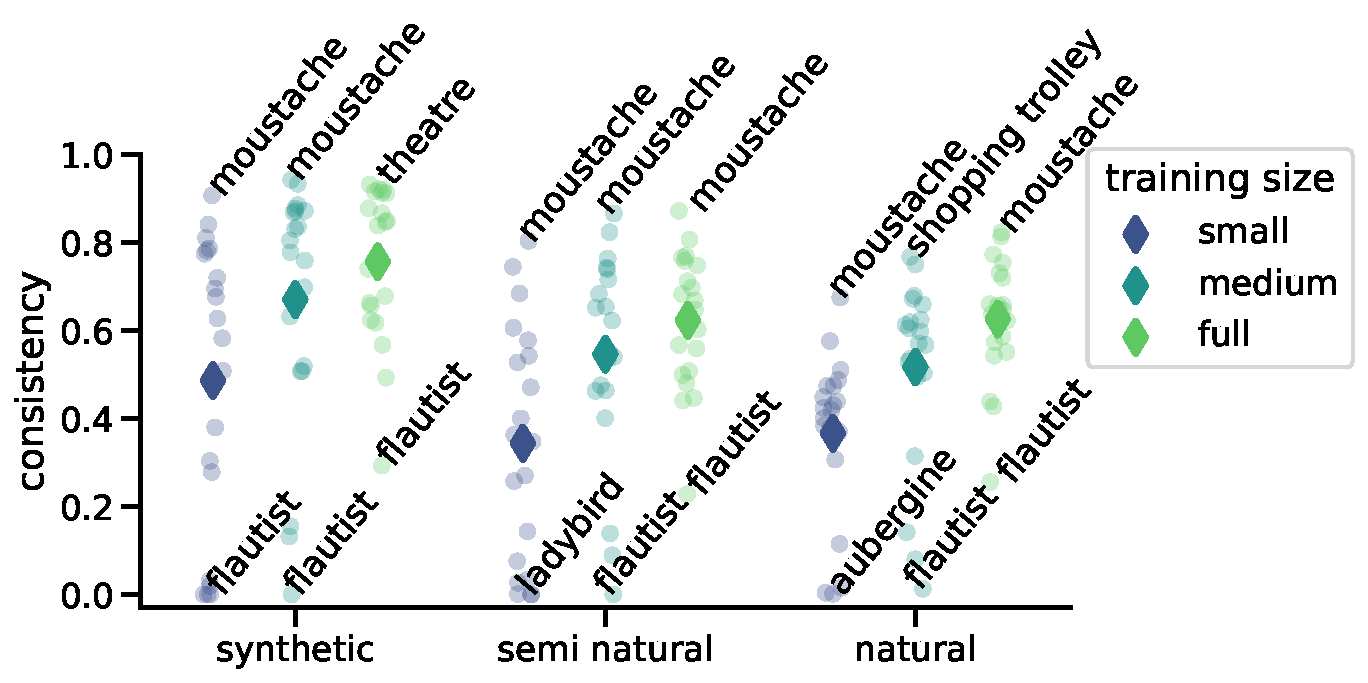
\includegraphics[width=\columnwidth]{figures/substitutivity/consistency.pdf}
    % \vspace{-0.3cm}
    \caption{}
        \vspace{-2mm}
    \label{fig:substitutivity}
    \end{subfigure}
% \end{figure}
% \begin{figure}
%V\centering
    \begin{subfigure}[b]{\columnwidth}
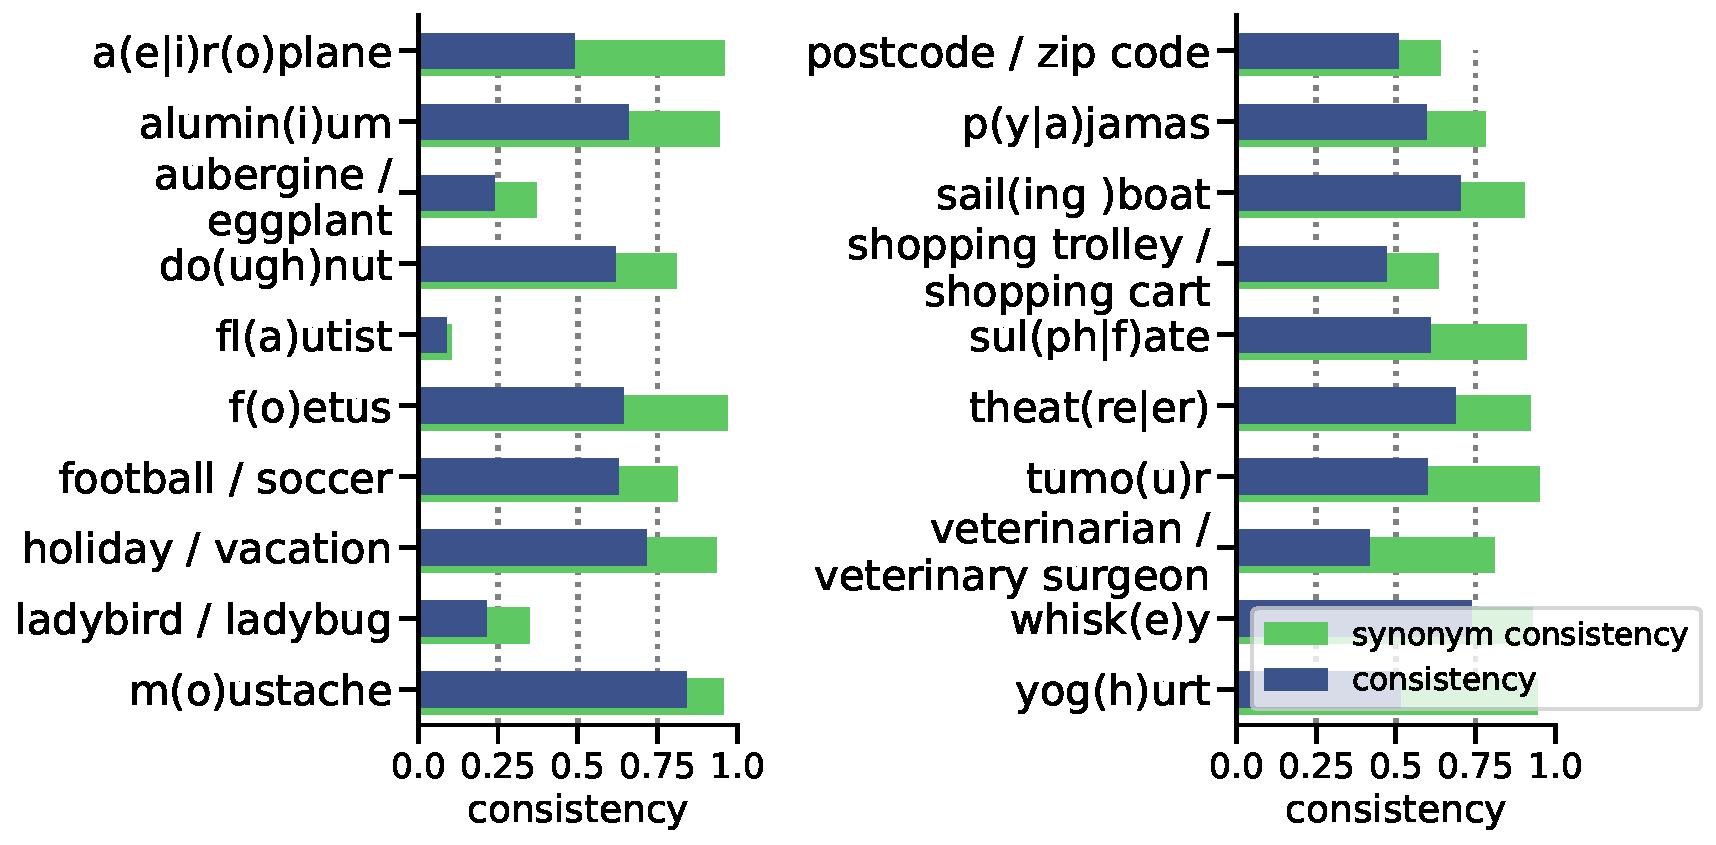
\includegraphics[width=\columnwidth]{figures/substitutivity/noun_consistency.pdf}
        \caption{}
        \vspace{-2mm}
\label{fig:per_synonym}
    \end{subfigure}
% \vspace{-0.3cm}
    \caption{(a) Consistency scores of synonyms (averaged $\diamond$, and per synonym $\circ$) for substitutivity per evaluation data type, for three training set sizes.
    %We annotate synonyms with the highest and lowest scores.
    (b) Consistency per synonym, measured using full sentences (in dark blue) or the synonym's translation only (in green), averaged over training dataset sizes and data types.}
    % \label{fig:substitutivity}
\vspace{-0.3cm}
\end{figure*}

\subsection{Systematicity}
\label{subsec:systematicity}

One of the most commonly tested properties of compositional generalisation is \textbf{systematicity} -- the ability to understand novel combinations made up from known components \citep[most famously,][]{lake2018generalization}.
In natural data, the number of potential recombinations to consider is infinite.
We chose to focus on recombinations in two sentence-level context-free rules: \texttt{S\;$\rightarrow$\;NP\;VP} and \texttt{S\;$\rightarrow$\;S\;CONJ\;S}.

\subsubsection{Experiments}
\paragraph{Test design}
\label{subsec:systematicity_test_design}
The first setup, \texttt{S\;$\rightarrow$\;NP\;VP}, concerns recombinations of noun and verb phrases.
We extract translations for input sentences from the templates from \S\ref{sec:data}, as well as versions of them with the (1) noun (NP $\rightarrow$ NP') or (2) verb phrase (VP $\rightarrow$ VP') adapted.
In (1), a noun from the NP in the subject position is replaced with a different noun while preserving number agreement with the VP.
In (2), a noun in the VP is replaced.
NP $\rightarrow$ NP' is applied to both synthetic and semi-natural data; VP $\rightarrow$ VP' only to synthetic data.
We use 500 samples per template per condition per data type.

The second setup, \texttt{S\;$\rightarrow$\;S\;CONJ\;S}, involves phrases concatenated using \exa{and}, and tests whether the translation of the second sentence is dependent on the first sentence.
We concatenate two sentences ($\text{S}_1$ and $\text{S}_2$) from different templates, and we consider again two different conditions.
First, in condition $\text{S}_1\rightarrow\text{S}^\prime_1$, we make a minimal change to $\text{S}_1$ yielding $\text{S}^\prime_1$ by changing the noun in its verb phrase.
In $\text{S}_1\rightarrow\text{S}_3$, instead, we replace $\text{S}_1$ with a sentence $\text{S}_3$ that is sampled from a template different from $\text{S}_1$.
We compare the translation of $\text{S}_2$ in all conditions.
For consistency, the first conjunct is always sampled from the synthetic data templates. 
The second conjunct is sampled from synthetic data, semi-natural data, or from natural sentences sampled from \textsc{OPUS} with similar lengths and word-frequencies as the semi-natural inputs.
We use 500 samples per template per condition per data type.
Figure~\ref{fig:systematicity_explanation} provides an illustration of the different setups experimented with.

\paragraph{Evaluation}
In artificial domains, systematicity is evaluated by leaving out combinations of `known components' from the training data and using them for testing purposes.
The necessary familiarity of the components (the fact that they are `known') is ensured by high training accuracies, and systematicity is quantified by measuring the test set accuracy.
If the training data is a natural corpus and the model is evaluated with a measure like BLEU in MT, this strategy is not available.
We observe that being systematic requires being consistent in the interpretation assigned to a (sub)expression across contexts, both in artificial and natural domains.
Here, we, therefore, focus on \textbf{consistency} rather than accuracy, allowing us to employ a model-driven approach that evaluates the model's systematicity as the consistency of the translations when presenting words or phrases in multiple contexts.

We measure consistency as the equality of two translations after accounting for anticipated changes.
For instance, in the \texttt{S\;$\rightarrow$\;NP\;VP} setup, two translations are consistent if they differ in one word only, after accounting for determiner changes in Dutch (\exa{de} vs\ \exa{het}).
In the evaluation of \texttt{S\;$\rightarrow$\;S\;CONJ\;S}, we measure the consistency of the translations of the second conjunct.

\subsubsection{Results}
Figure~\ref{fig:systematicity} shows the results for the \texttt{S\;$\rightarrow$\;NP\;VP} and \texttt{S\;$\rightarrow$\;S\;CONJ\;S} setups (numbers available in Appendix~\ref{ap:systematicity}).
The average performance for the natural data closely resembles the performance on \textit{semi-}natural data, suggesting that the increased degree of control did not severely impact the results obtained using this generated data.\footnote{In our manual analysis (\S\ref{sec:manual_analysis}), however, we did observe a slightly different distribution of changes between these setups.}
In general, the consistency scores are low, illustrating that models are prone to changing their translation of a (sub)sentence after small (unrelated) adaptations to the input.
It hardly matters whether that change occurs in the sentence itself (\texttt{S\;$\rightarrow$\;NP\;VP}), or in the other conjunct (\texttt{S\;$\rightarrow$} \texttt{S\;CONJ\;S}), suggesting that the processing of the models is not local as assumed in strong compositionality.
Models trained on more data seem more locally compositional, a somewhat contradictory solution to achieving compositionality, which, after all, is assumed to underlie the ability to generalise usage from \emph{few} examples \citep{lake2019human}.
This trend is also at odds with the hypothesis that inconsistencies are a consequence of the natural variation of language, which models trained on \emph{more} data are expected to better capture.


\subsection{Substitutivity}
\label{subsec:substitutivity}

Under a local interpretation of the principle of compositionality, synonym substitutions should be meaning-preserving: substituting a constituent in a complex expression with a synonym should not alter the complex expression's meaning, or, in the case of MT, its translation.
Here, we test to what extent models' translations abide by this principle, by performing the \textbf{substitutivity} test from \citet{hupkes2020compositionality}, that measures whether the outputs remain consistent after synonym substitution.

\subsubsection{Experiments}
To find synonyms -- source terms that translate into the same target terms -- we exploit the fact that OPUS contains texts both in British and American English.
Therefore, it contains synonymous terms that are spelt different -- e.g.\ \exa{doughnut} / \exa{donut} -- and synonymous terms with a very different form -- e.g.\ \exa{aubergine} / \exa{eggplant}.
We use 20 synonym pairs in total (see Figure~\ref{fig:per_synonym}).

\paragraph{Test design}
Per synonym pair, we select natural data from OPUS in which the terms appear and perform synonym substitutions.
Thus, each sample has two sentences, one with the British and one with the American English term.
We also insert the synonyms into the synthetic and semi-natural data using 500 samples per synonym pair per template, through subordinate clauses that modify a noun -- e.g. ``the king \textit{that eats the doughnut}''.
In Appendix~\ref{ap:substitutivity}, Table~\ref{tab:substitutivity_appendix}, we list all clauses used.

\paragraph{Evaluation}
Like systematicity, we evaluate substitutivity using the consistency score, expressing whether the model translations for a sample are identical.
We report both the full sentence consistency and the consistency of the synonyms' translations only, excluding the context.
Cases in which the model omits the synonym from both translations are labelled as consistent if the rest of the translation is the same for both input sequences.

\subsubsection{Results}
In Figure~\ref{fig:substitutivity}, we summarise all substitutivity consistency scores (tables are in Appendix~\ref{ap:substitutivity}).
We observe trends similar to the systematicity results: models trained on larger training sets perform better and synthetic data yields more consistent translations compared to (semi-)natural data.
We further observe large variations across synonyms, for which we further detail the performance aggregated across experimental setups in Figure~\ref{fig:per_synonym}.
The three lowest scoring synonyms -- \exa{flautist}, \exa{aubergine} and \exa{ladybug} -- are among the least frequent synonyms (see Appendix~\ref{ap:substitutivity}), which stresses the importance of frequency for the model to pick up on synonymy.

In Figure~\ref{fig:per_synonym}, we show both the regular consistency and the consistency of the synonym translations, illustrating that a substantial part of the inconsistencies are due to varying translations of the context rather than the synonym itself, stressing again the non-local processing of the models.

\subsection{Global compositionality}
\label{subsec:global_compositionality}

In our final test, we focus on exceptions to compositional rules.
In natural language, typical exceptions that constitute a challenge for local compositionality are \emph{idioms}.
For instance, the idiom ``raining cats and dogs'' should be treated globally to arrive at its meaning of heavy rainfall.
A local approach would yield an overly literal, non-sensical translation (``het regent katten en honden'').
When a model's translation is too local, we follow \citet{hupkes2020compositionality} in saying that it \textbf{overgeneralises}, or, in other words, it applies a general rule to an expression that is an exception to this rule.
Overgeneralisation indicates that a language learner has internalised the general rule \citep[e.g.][]{penke2012dual}.

\subsubsection{Experiments}
We select 20 English idioms for which an accurate Dutch translation differs from the literal translation from the English MAGPIE corpus \citep{haagsma2020magpie}.
Because acquisition of idioms is dependent on their frequency in the corpus, we use idioms with at least 200 occurrences in OPUS based on exact matches, for which over 80\% of the target translations does not contain a literal translation.

\paragraph{Test design}
Per idiom, we extract \textit{natural} sentences containing the idiom from OPUS. 
For the synthetic and semi-natural data types, we insert the idiom in 500 samples per idiom per template, by attaching a subordinate clause to a noun -- e.g.\ ``the king \emph{that said `I knew the formula \textbf{by heart}'}''. 
The clauses used can be found in Appendix~\ref{ap:global_compositionality}, Table~\ref{tab:overgeneralisation_appendix}.

\paragraph{Evaluation}
Per idiom, we assess how often a model overgeneralises and how often it translates the idiom globally. 
To do so, we identify keywords that indicate that a translation is translated locally (literal) instead of globally (idiomatic).
If the keywords' literal translations are present, the translation is labelled as an overgeneralised translation. 
For instance, for ``by heart'', the presence of ``hart'' (``heart'') suggests a literal translation. An adequate paraphrase would say ``uit het hoofd'' (``from the head'').
See Appendix~\ref{ap:global_compositionality}, Table~\ref{tab:overgeneralisation_appendix}, for the full list of keywords.
We evaluate overgeneralisation for ten intermediate training checkpoints.

\begin{figure}
    \centering
    \begin{subfigure}[b]{\columnwidth}\centering
    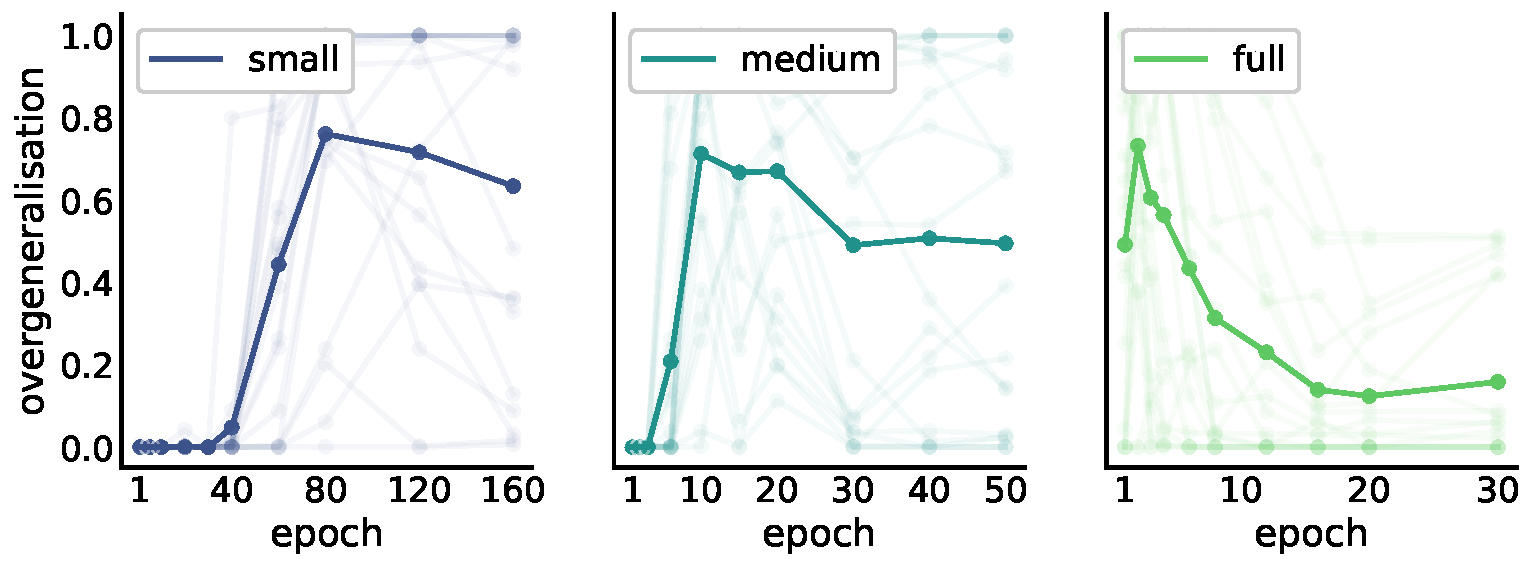
\includegraphics[width=\textwidth]{figures/global_compositionality/synthetic.pdf}
    \caption{Synthetic}
    \end{subfigure}
    \begin{subfigure}[b]{\columnwidth}\centering
    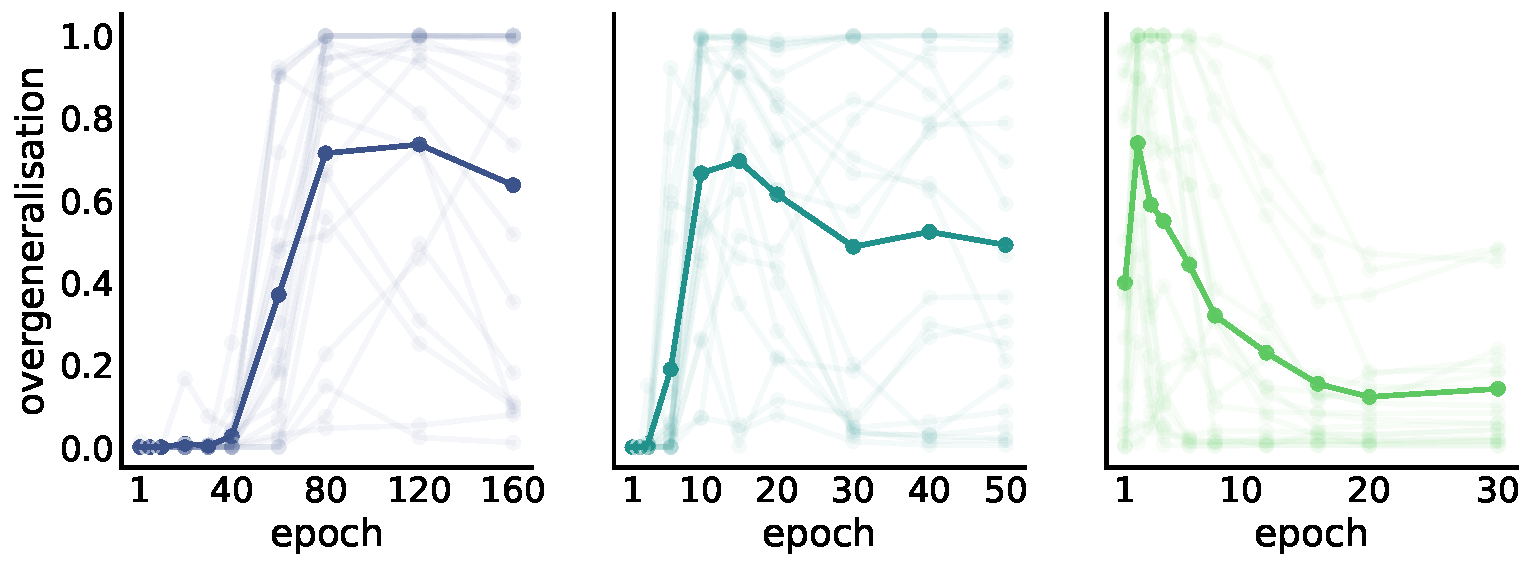
\includegraphics[width=\textwidth]{figures/global_compositionality/semi_natural.pdf}
    \caption{Semi-Natural}
    \end{subfigure}
    \begin{subfigure}[b]{\columnwidth}\centering
    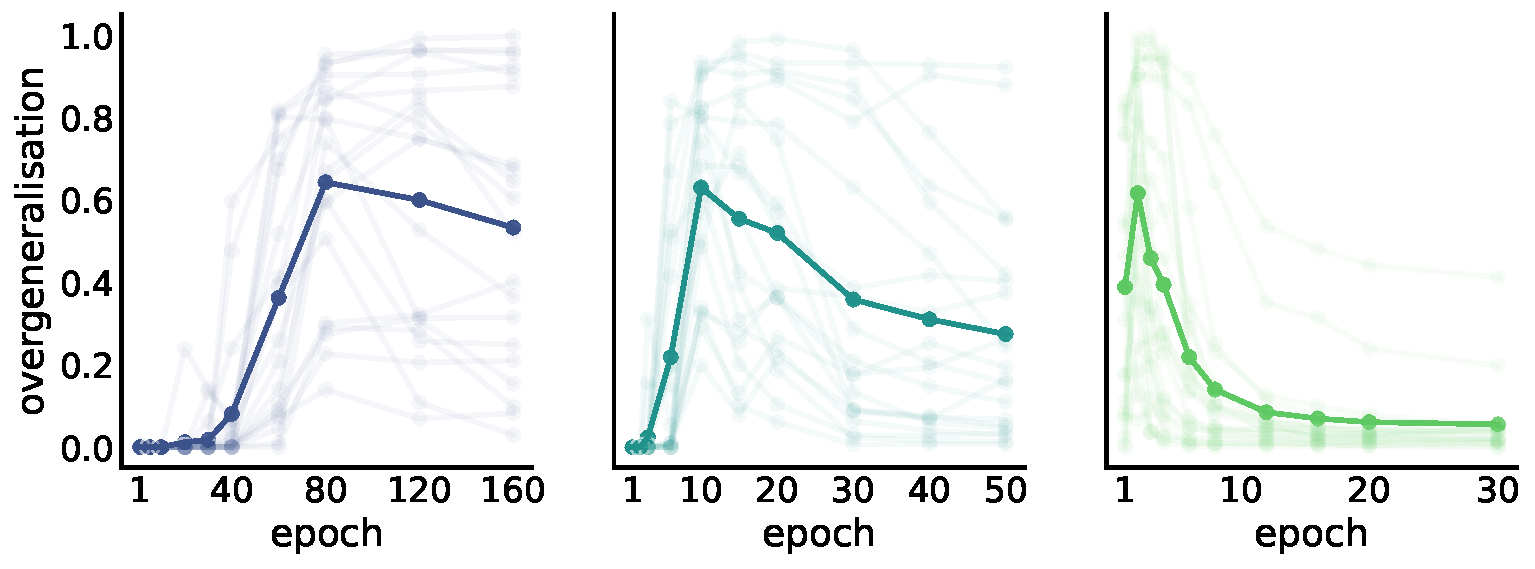
\includegraphics[width=\textwidth]{figures/global_compositionality/natural.pdf}
    \caption{Natural}
    \end{subfigure}
    \caption{Visualisation of overgeneralisation for idioms throughout training, with a line per idiom and the overall mean. Overgeneralisation occurs early on in training and precedes memorisation of idioms' translations.
    The colours indicate different training dataset sizes.}
    \label{fig:global_compositionality}
    \vspace{-0.3cm}
\end{figure}

\subsubsection{Results}
In Figure~\ref{fig:global_compositionality}, we report our results.\footnote{Note that epochs consist of different numbers of samples: 1M, 8.6M and 69M for small, medium and full. Appendix~\ref{ap:global_compositionality} further details numerical results per idiom.}
For all evaluation data types and all training set sizes, three phases can be identified.
Initially, the translations do not contain the idiom's keyword, not because the idiom's meaning is paraphrased in the translation, but because the translations consist of high-frequency words in the target language only. 
Afterwards, overgeneralisation peaks: the model emits a very literal translation of the idiom.
Finally, the model starts to memorise the idiom's translation.
This is in accordance with results from \citet{hupkes2020compositionality}, and earlier results presented in the past tense debate by -- among others -- \citet{rumelhart1986learning}.

Although the height of the overgeneralisation peak is similar across evaluation data types and training set sizes, overgeneralisation is more prominent in converged models trained on smaller datasets than it is in models trained on the full corpus.\footnote{Convergence is based on BLEU scores for validation data.}
In addition to training dataset size, the type of evaluation data used also matters: there is more overgeneralisation for synthetic and semi-natural data compared to natural data, stressing the impact of the context in which an idiom is embedded.
The extreme case of a context unsupportive of an idiomatic interpretation is a sequence of random words. To evaluate the hypothesis that this yields local translations, we surround the idioms with ten random words.
The results (Appendix~\ref{ap:global_compositionality}, Table~\ref{tab:overgeneralisation_appendix}) indicate that, indeed,  when the context provides no support at all for a global interpretation, the model provides a local translation for nearly all idioms.
Overall, the results of this test provide an interesting contrast with our substitutivity and systematicity results: where in those tests, we saw processing that was \emph{less local} than we expected, here, the behaviour shown by the models is instead \emph{not global enough}.


\section{Manual analysis}
\label{sec:manual_analysis}

Our systematicity and substitutivity results demonstrate that models are not behaving compositional according to a strict definition of compositionality.
However, we ourselves have argued that strict compositionality is not always appropriate to handle natural language.
A reasonable question to ask is thus: are the inconsistencies we marked as non-compositional actually incorrect?

\paragraph{Annotation setup} 
To address this question, we perform a manual analysis.
We annotate 900 inconsistent translation pairs of the systematicity and substitutivity tests to establish whether the inconsistencies are benign or concerning.
We consider four different types of changes:
\begin{enumerate}[noitemsep,topsep=0pt]
\item cases of \textit{rephrasing}, where both translations are equally (in)correct;
\item changes reflecting different interpretations of \textit{source ambiguities};
\item cases in which one of the two translations contains an \textit{error};
\item \textit{formatting} (mostly punctuation) changes.
\end{enumerate}
For substitutivity samples, we also annotate whether the changes are related to the translation of the synonym, where we distinguish cases where
\begin{enumerate}[noitemsep,topsep=0pt]
\item[i.] one of the synonym translations is incorrect;
\item[ii.] both are incorrect but in a different manner;
\item[iii.] both are correct but translated differently;
\item[iv.] one synonym remains untranslated.
\end{enumerate}
We annotate all changes observed per pair and report the relative frequency per class. 
We summarise the results, aggregated over different training set sizes and the three data types, in Figure~\ref{fig:manual_analysis_summary}.
For a more elaborate analysis and a breakdown per model and data type, we refer to Appendix~\ref{app:man_analysis}.

\begin{figure}
	\begin{subfigure}[b]{\columnwidth}
		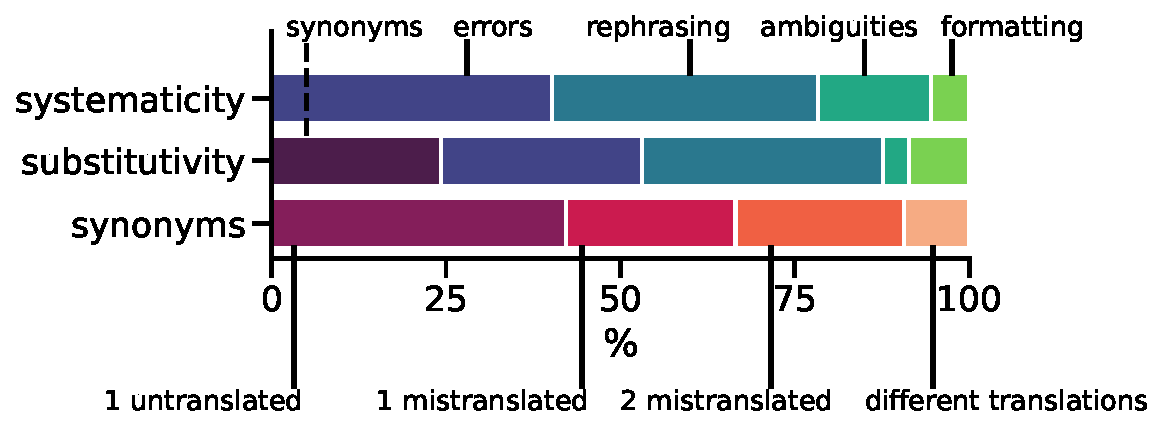
\includegraphics[width=\textwidth]{figures/analysis_appendix/summary_analysis.pdf}
	\end{subfigure}
	\caption{Relative frequencies of manually labelled inconsistencies in translations, averaged over data types and training set sizes.
	         The `synonyms' distribution further details the category `synonyms' from row two.}
	\label{fig:manual_analysis_summary}
	\vspace{-.3cm}
\end{figure}


\paragraph{Results}
In the systematicity test, 40\% of the marked inconsistencies reflects wrongfully translated parts in one of the two sentences, whereas 38\% contains examples of rephrasing, 16\% reflects ambiguities in the source sentences and 6\% is caused by formatting differences. 
For substitutivity, most inconsistencies are similar to the ones observed in systematicity: only 24\% involves the synonyms' translations, where one of them being untranslated was the most frequent category.
 
The distribution of these types of inconsistencies differ strongly per training data type.
For models trained on less data, inconsistencies are more likely to represent errors, whereas models trained on more data rephrase more often. 
This result emphasises that for lower-resource settings, being compositional is particularly relevant.

Another demonstration of this relevance comes from the observation that although models \textit{can} emit correct translations for nearly all synonyms,\footnote{Apart from the model with the small training dataset that cannot translate \exa{flautist} and \exa{ladybug}.}
they do not always do so, depending on the context.
To give a peculiar example: in ``The child admires the king that eats the \{doughnut, donut\}'', the snack was occasionally translated as ``ezel'' (\exa{donkey}).

\paragraph{Robustness and predictability}
Finally, we would like to stress that while rephrasing often might seem benign rather than concerning from the perspective of emitting adequate translations, its harmlessness still deserves some thought.
There is a fine line between rephrasing and mistranslating: whether ``the \textit{single largest} business establishment'' is referred to as ``de grootste'' (\exa{the largest}) or ``de enige grootste'' (\exa{the only largest}) may make or break a translation. 
Furthermore, if changes are unrelated to the contextual change (e.g. replacing ``soccer'' with ``football''), this can be undesirable from a robustness and reliability perspective.
This point becomes even more pronounced in cases where both translations are correct but have a different meaning.
To analyse the extent to which inconsistencies are actually unmotivated, we investigated if we could trace them back to the contextual change, in particular focusing on whether changing synonyms from British to American spelling or vice versa might trigger a change in style or tone.
We could not find evidence of such motivations, indicating that even correct cases of rephrasing were not caused by contextual changes that were \emph{necessary} to take into account.


\section{Related Work}
\vspace*{-2mm}
% \JC{Ref Sec 2. more thorough related work }
While Sec.\,\ref{sec: primer_MU} provides a summary of related works concerning exact and approximate unlearning methods and metrics,  a more comprehensive review  is provided below.

\noindent \textbf{Machine unlearning.}
%% sparsity in unlearning.
\iffalse 
{\MU} was first introduced in   \cite{cao2015towards}, which aims to make  an ML model to `forget'  data points upon completion of training.   {\MU}  was originally used  to prevent the leakage of  data privacy  from the trained model,   
in particular in coming forth with legislation like  General Data Protection Regulation (GDPR) \cite{hoofnagle2019european} and  California Consumer Privacy Act (CCPA) \cite{pardau2018california}. 
A straightforward approach  to unlearning is to retrain the model from scratch (\textit{i.e.}, {\retrain}) after removing the forgetting dataset from the original training set. Although {\retrain} yields the ground-truth unlearning strategy, it is least efficient in computation. Thus,   approximate but fast unlearning    becomes a significant research focus nowadays; examples include \cite{golatkar2020eternal,warnecke2021machine,graves2021amnesiac,thudi2021unrolling,becker2022evaluating,izzo2021approximate} as we reviewed in Sec.\,\ref{sec: primer_MU}. 
\fi 
In addition to exact and approximate unlearning methods as we have reviewed in Sec.\,\ref{sec: primer_MU}, there  exists other literature aiming to  develop  the probabilistic notion of unlearning \cite{ginart2019making,guo2019certified,neel2021descent,ullah2021machine,sekhari2021remember}, in particular through the lens of differential privacy (DP) \cite{dwork2006our}. Although DP enables unlearning  with provable error guarantees, %\cite{guo2019certified,neel2021descent,ullah2021machine,sekhari2021remember}, 
they typically require strong model and algorithmic assumptions and could lack effectiveness when facing practical  adversaries, \textit{e.g.}, membership inference attacks. Indeed, evaluating {\MU}  is far from trivial \cite{becker2022evaluating,thudi2022necessity,thudi2021unrolling}.  %as we described in Sec.\,\ref{sec: primer_MU}. 
Furthermore, the attention on  {\MU} has also   been raised in   different learning paradigms, \textit{e.g.}, federated learning   \cite{wang2022federated,liu2022right}, graph neural networks \cite{chen2022graph,chien2022certified,cheng2023gnndelete}, and adversarial ML \cite{marchant2022hard,di2022hidden}.
In addition to   preventing the leakage of  data privacy  from the trained models, the concept of {\MU} has also inspired  other emergent applications such as adversarial defense against backdoor attacks \cite{liu2022backdoor,warnecke2021machine} that we have studied and erasing image concepts of conditional generative models \cite{gandikota2023erasing,zhang2023forget}.
%Moreover, in addition to its primary applications, we have demonstrated \MU's potential in mitigating backdoor attacks \cite{liu2022backdoor}, as well as in augmenting the performance of transfer learning \cite{jain2022data}. These diverse applications underscore the versatility and utility of machine unlearning in various domains.

 


\noindent \textbf{Understanding data influence.}
The majority of {\MU} studies are motivated by data privacy. Yet, they  also closely relate to another line of research on understanding data influence in ML. For example, the influence function approach \cite{koh2017understanding} has been used as an algorithmic backbone of many unlearning methods  \cite{warnecke2021machine,izzo2021approximate}. From the viewpoint of data influence, {\MU}  has been used in the use case of adversarial defense against data poisoning backdoor attacks \cite{liu2022backdoor}. Beyond unlearning, evaluation of data influence  has also been studied in  fair learning  \cite{sattigeri2022fair,wang2022understanding},  transfer learning  \cite{jain2022data}, and   dataset pruning \cite{borsos2020coresets,yang2022dataset}. 
%to improve  the efficiency of ML. 


% It can also be viewed as a method of understanding dataset influence
% %\PR{dataset influence?}
% in model training


%%  In [16], Liu et al., for instance, utilize forgetting in order to remove backdoors that were induced into a model.

\noindent \textbf{Model pruning.}
%\iffalse 
The deployment constraints on \textit{e.g.}, computation, energy, and memory   necessitate the pruning of
today's ML models, \textit{i.e.}, promoting their weight sparsity. %\cite{han2015deep,chen2021lottery,frankle2018lottery,frankle2020linear,ma2021sanity,zhang2022advancing}.
%\fi 
The vast majority of existing works \cite{han2015deep,chen2021lottery,frankle2018lottery,frankle2020linear,ma2021sanity,zhang2022advancing,blalock2020state} focus on  developing model pruning methods that can strike a graceful balance between model's generalization and sparsity.
%the  generalization ability of pruned models against its sparsity; see the seminal work \cite{blalock2020state}. 
In particular, the existence of LTH (lottery ticket hypothesis) \cite{frankle2018lottery} demonstrates 
the feasibility of co-improving the model's generalization  and efficiency (in terms of sparsity) \cite{liu2018rethinking,tanaka2020pruning,wang2020picking,lee2018snip,zhang2023data}. 
%has been empirically justified  by LTH (lottery ticket hypothesis) \cite{frankle2018lottery},
\iffalse 
This has inspired 
many different kinds of pruning methods \cite{liu2018rethinking,tanaka2020pruning,wang2020picking,lee2018snip}. 
\fi 
In addition to generalization, model sparsity   achieved by pruning   can also be  leveraged to improve other performance metrics, such as   robustness \cite{sehwag2020hydra,chen2022quarantine,diffenderfer2021winning}, model explanation  \cite{wong2021leveraging,chen2022can},
%model connectivity \cite{frankle2020linear}, 
and privacy \cite{huang2020privacy,wang2020against,luo2021scalable,gong2020privacy}.

\iffalse 
out-of-distribution generalization \cite{diffenderfer2021winning}. 
In particular, the   relevant work to ours is model pruning for privacy-preserving learning \cite{huang2020privacy,wang2020against,luo2021scalable,gong2020privacy}. Yet,  nearly all the existing works  focus on how sparsity impacts data privacy, \textit{e.g.}, evaluated using MIAs (membership inference attacks) 
%against pruned models on training data points 
\cite{bagmar2021membership,yuan2022membership}. This is akin to MIA evaluation on the retained dataset in our work. Thus, pruning for privacy cannot   provide   a holistic and in-depth understanding of  how pruning  impacts {\MU}.  
\fi 

\iffalse
In addition,
a few recent works   \cite{wang2022federated,ye2022learning} attempt to draw insights from pruning for unlearning. In \cite{wang2022federated},  pruning channels of a  neural network shows   unlearning benefits in federated learning. And in \cite{ye2022learning}, filter pruning is introduced in lifelong learning to detect pruning identified exemplars (PIEs)   \cite{hooker2019compressed} that  are easy to forget. 
Different from the aforementioned literature to customize  pruning   for specific unlearning applications,  our work for the first time explores and exploits the connection between model pruning and unlearning systematically and in-depth. 
\fi 


%or membership inference attack and defense 

%\textsc{Grasp}\,\cite{wang2020pick}, \textsc{Snip}\,\cite{lee2018snip}, 

%%% pruning vs. privacy
%\paragraph{Pruning for.}




\section{Discussion}

\subsection{Performance \& Model Size}\label{sec:disscusion:perf}

As seen in \Cref{section:eval}, \emph{wide Transformer networks typically offer equal or greater accuracy} on a range of classification tasks with different sequence lengths.
The impact of wider and shallower networks on accuracy is slightly influenced by the attention type, with some having more significant changes in accuracy than others.
There was no significant difference between convergence time during training for wide and deep models.
Each attention mechanism on each task achieved its best validation accuracy after roughly the same number of training steps for all model aspect ratios.

Whilst the total number of parameters involved in the attention layers remains constant amongst different aspect ratios, the overall number of parameters decreases.
This is due to the feed-forward network (FFN) part of the Transformer layer remaining unaltered as we change the models width.
The models with fewer layers have fewer FFN blocks, and so fewer parameters.

The deepest IMDb byte level classification and Listops models are typically 230MiB, with the widest models typically being 110MiB, only 48\% of the size.
On token level classification and document matching the sizes are closer.
Averaged across all tasks and attention mechanisms, the widest models are 71\% the size of the deepest models.
A full table of model sizes for the deepest and widest models across all tasks and attention types is given in \Cref{table:model_sizes}, in \Cref{appendix:model_size}.


\subsection{Latency}\label{sec:disscusion:lat}

As the number of layers in a model decrease, so does the number of dependencies in the computation graph.
Because of this a forward pass through the model will have lower latency, though overall throughput may remain unchanged.
For systems which require very low latency, such as real time processing in autonomous driving \citep{talpes2020compute}, this feature could make a wide single layer model more desirable than an equally accurate deep one.

We measure inference latency for the deepest and widest models for each task and attention type on a CPU with a single input, and on a GPU with a batch input.
Experimental details are given in \Cref{appendix:latency} along with raw numbers in \Cref{table:cpu_latency,table:gpu_latency}.
We find that on average the widest models are $3.1 \times$ faster on a CPU and $1.9 \times$ faster on a GPU than the deepest models.
The speed-up is consistent across all tasks and attention types.


\subsection{Interpretability}\label{sec:disscusion:interp}

\begin{figure}[hbt]
    \centering
    \begin{subfigure}{.35\textwidth}
        \centering
        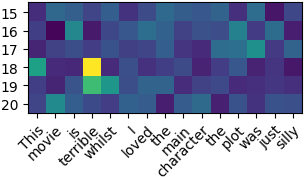
\includegraphics[height=0.12\textheight]{imgs/example_1_cropped.png}
        \caption{Prediction: strongly negative}
        \label{fig:wide_attention_1}
    \end{subfigure}
    \hspace{.05\textwidth}
    \begin{subfigure}{.55\textwidth}
        \centering
        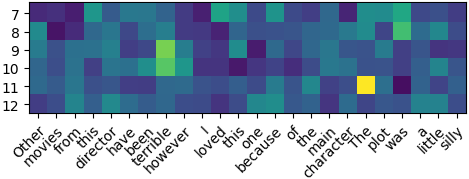
\includegraphics[height=0.12\textheight]{imgs/example_2_cropped.png}
        \caption{Prediction: weakly positive}
        \label{fig:wide_attention_2}
    \end{subfigure}
    \caption{The attention weights across a selection of heads with predicted classification for the single layer IMDb token level text classification Transformer model on two unseen and similar examples.}
    \label{fig:wide_attention}
\end{figure}

Interpretability is increasingly important and a very active area of machine learning research \citep{interpret1, interpret2}, especially when it comes to fairness.
By having more easily inspect-able models, we can see the reasons for a given classification.
For example, was a decision based on the mention of a protected characteristic, such as race or gender?

In a Transformer-based architecture, the attention heads in a layer can be inspected during inference to see what connections between input features that head found important.
For deep networks, many layers means it can often become unclear what the final output was actually based on \citep{tfm_interpret}.
For a single layer wide network, interpretability is far easier as only one layer needs to be inspected.
Thus what was considered important for the final output is much clearer.

In \Cref{fig:wide_attention}, we can see the attention weights across some of the heads of the widest token level text classification Transformer model, as well as the predicted class for two different example inputs that have been designed to be similar.
\Cref{fig:wide_attention} includes a subset of the total number of heads, for all 48 heads see \Cref{fig:wide_attention_full} in \Cref{appendix:attention}.

We can see the review on the left has been confidently assigned as a negative review, and from the attention weights we can see that this is due to the model recognising the relevance of the word ``terrible".
The review on the right has been less confidently assigned as positive.
From the attention weights we can see it has recognised words such as ``terrible", but the largest weight is on ``The". This explains why the model might not be confident in its positive prediction because it hasn't realised the importance of the word ``loved".


\subsection{Theoretical Explanations of Outliers}\label{sec:theory}

Most attention mechanisms usually have up to a 0.5\% increase in accuracy when going wider with two notable exceptions.
Longformer \citep{longformer} typically performs significantly better when deep, and Sinkhorn \citep{sinkhorn} typically performs significantly better when wide.

For Longformer we only use sliding window attention, with a width of 512.
This means, particularly for the longer tasks, each input feature can only have attention computed between it and its neighbours.
For deeper models, features can propagate and so this limitation is reduced.
However, single layer models suffers a performance penalty.

Sinkhorn works similarly to local attention, where the input sequence is divided into blocks.
Unlike local attention, which computes attention within these blocks, Sinkhorn sorts them and computes attention between the original block and the newly sorted block.
This sorting mechanism is learn-able per head., thus each head can learn a different sorting strategy.
For lots of heads this maximises the overall chance of important long range connections within the input sequence being attended to.


\subsection{Vision Transformer}\label{sec:discussion:vit}

There is a growing interest in applying Transformers to computer vision \citep{wang2021pyramid,wang2022pvt,liu2021swin,dosovitskiy2020image}.
We tested the Pyramid Vision Transformer model (PVT-V2-B1) \citep{wang2022pvt} and its wider variants on the CIFAR10 dataset \citep{krizhevsky2014cifar}.
The PVT-V2-B1 model has four stages with each stage containing two attention layers.
We then replace the two attention layers at each stage with a single wide attention layer.
The detailed architecture of the PVT-V2-B1 model and its wider variants are shown in \Cref{tab:vit}.
The first wider variant (Wide) matches the total number of heads to the original PVT-V2-B1 model, whereas the later variant (Wide-V2) contains a larger embedding size and more heads.
This is a closer match to the original model in terms of the model size.

\begin{table*}[!h]
	\caption{
		Performance of the original Pyramid Vision Transformer (PVT) and its wider alternatives on the CIFAR10 dataset.
		The original model (PVTV2-B1) has 4 stages, each stage contains two attention layers.
		((1, 1), (2, 2), (5, 5), (8, 8)) describes the original model,
		for instance, the first block contains two layers with a single head each, represented as (1, 1).}
	\centering
	\begin{tabular}{c|ccc}
	\toprule
	\textbf{Name}
	& \textbf{Configuration}
	& \textbf{Accuracy}
	& \textbf{Parameters} \\
	\midrule
	Baseline
	& $((1, 1), (2, 2), (5, 5), (8, 8))$
	& $95.59 \pm 0.99$	
	& $13.5$M	 \\
	Wide
	& $((2), (4), (10), (16))$
	& $94.54 \pm 0.31$	
	& $7.7$M	 \\
	Wide-V2
	& $((4), (8), (20), (32))$
	& $94.94 \pm 0.20$	
	& $12.6$M	 \\
	\bottomrule
	\end{tabular}
	\label{tab:vit}
\end{table*}


\Cref{tab:vit} illustrates that the wider variants do not outperform the original PVT-V2-B1 model.
Intuitively, spatial features play an important role in vision tasks.
The average pooling layer that comes before each attention layer is a crucial component of the PVT model.
With only a single wide layer, this pooling layer is not capturing as much spatial information as before.
The usage of a single wide attention layer in vision Transformers is constrained by the fact that the majority of these vision Transformers still use pooling or convolution layers before the attention.



\subsection{Mixed Attention}

\begin{table}[htb]
    \caption{Test accuracy for each task for wide and deep mixed attention models alongside the averages of all homogeneous models, and the best performing homogeneous model for that task.}
    \label{table:mixed}
    \begin{center}
        \begin{tabular}{l | l l l | l l l}
            \toprule
            \multirow{2}{*}{\bf Task} & \multicolumn{3}{c}{\bf Deepest} & \multicolumn{3}{c}{\bf Widest} \\
            & Hom. Avg & Hom. Best & Mixed & Hom. Avg & Hom. Best & Mixed \\
            \midrule
            IMDb Token Level & 84.8 & 87.0 & 87.3 & 84.7 & \textbf{88.0} & 86.8 \\
            IMDb Byte Level & 61.3 & 64.5 & 60.1 & 60.7 & \textbf{64.8} & 63.0 \\
            Listops & 34.2 & 37.1 & 37.1 & 35.7 & 37.7 & \textbf{38.0} \\
            Document Matching & 63.9 & 71.1 & - & 64.0 & \textbf{72.3} & 66.9 \\
            \bottomrule
        \end{tabular}
    \end{center}
\end{table}

With wider attention layers, the advantages of mixing attention methods becomes more viable.
We test a uniform mixture of attentions in both wide and deep variants to see how these models perform.
For each layer we use an equal mix of the following attention mechanisms: BigBird, Linear Transformer, Linformer, Local, Longformer, Performer, Sparse Transformer, and Synthesizer.

We omit Sinkhorn since it does not use the [CLS] token for classification like the other attention methods.
We also omit vanilla attention so that we have a total of 8 mechanisms, and our overall attention operation is efficient (sub-quadratic time and space complexities).

We initialise a separate multiheaded attention block for each mechanism and average all of their outputs when going back to the sequence features.
The number of attention heads in each block is scaled such that the total number equals that of the homogeneous model.
For example in the 6 layers, 8 heads configuration, each of our attention blocks has a single head.
In the 1 layer 48 heads configuration, each has 6 heads.

Results are given in \Cref{table:mixed}.
Deep mixed attention on matching is not tested as there are not enough heads to include every attention mechanism.
We also include in this table repeats of the averages and bests for each task across all attention mechanisms.
From the table we can see that even with mixed attention, the widest single layer models typically perform better (IMDb byte level, Listops) or only marginally worse (IMDb token level) than the deep Transformer models.
Whilst beating the averages, all the best mixed models except Listops are outperformed by one of the homogeneous attention models in its widest configuration.
The widest mixed model on Listops however points towards mixed attention having possible advantages over homogeneous attention for certain tasks.





\section*{Acknowledgements}

We thank Sebastian Riedel, Douwe Kiela, Thomas Wolf, Khalil Sima'an, Marzieh Fadaee, Marco Baroni, Brenden Lake and Adina Williams for providing feedback on this draft and our work in several different stages of it.
We thank Michiel van der Meer for contributing to the initial experiments that led to this paper.
A special thanks goes to Angela Fan, who assisted us at several points to get the ins and outs of training large MT models and double-checked several steps of our pipeline and to our ARR reviewers, who provided amazingly high quality feedback.
VD is supported by the UKRI Centre for Doctoral Training in Natural Language Processing, funded by the UKRI (grant EP/S022481/1) and the University of Edinburgh.



\bibliography{references,anthology}
\bibliographystyle{acl_natbib}

\clearpage

\appendix
\begin{appendices}

% \setcounter{lemma}{0}
%     \renewcommand{\thelemma}{\Alph{section}\arabic{lemma}}
    
\begin{comment}
\end{comment}

{\colorred 
\section{Compatible Value Function}
\label{app:comp_v}

The original policy gradient with compatible value function is stated as follow. 
\begin{theorem}
[\cite{sutton1999policy}]
Let $Q_w$ be a state-action function with parameter $w$ and $\pi_\theta$ be a policy function with parameter $\theta$. 
If $Q_w$ satisfies $\mathbb{E}_{\pi} [(Q^\pi - Q_w) \nabla_w Q_w] = 0$ and 
$\nabla_w Q_w = \nabla_\theta \log \pi_\theta,$
then $$\nabla_\theta \mathcal{J} = \mathbb{E}_\pi [Q_w \nabla_\theta \log \pi_\theta].$$
\label{thm:pg_fa}
\end{theorem}
If we let $w = \theta$ in Theorem \ref{thm:pg_fa}, where $Q_w$ and $\pi_\theta$ share parameters, we have the following theorem. 
\begin{theorem}
Let $Q_\theta$ be a state-action function with parameter $\theta$ and $\pi_\theta$ be a policy function with parameter $\theta$. 
If $Q_\theta$ satisfies $\mathbb{E}_{\pi} [(Q^\pi - Q_\theta) \nabla_\theta Q_\theta] = 0$ and 
$\nabla_\theta Q_\theta = \nabla_\theta \log \pi_\theta,$
then $$\nabla_\theta \mathcal{J} = \mathbb{E}_\pi [Q_\theta \nabla_\theta \log \pi_\theta].$$
\label{thm:pg_fa2}
\end{theorem}
Define 
$$\chi \overset{def}{=} \mathbb{E}_\pi [\cos <\nabla_\theta Q_\theta, \nabla_\theta \log \pi_\theta>].$$
We show that $\chi = 1$ is the necessary condition for the compatible condition $\nabla_\theta Q_\theta = \nabla_\theta \log \pi_\theta$. 
\begin{theorem}
i) If $\nabla_\theta Q_\theta \propto \nabla_\theta \log \pi_\theta$ for all states, then $\chi = 1$.

ii) If $\chi = 1$, then $\nabla_\theta Q_\theta \propto \nabla_\theta \log \pi_\theta$ for all states. 
\label{thm:connect_cond}
\end{theorem}
By Theorem \ref{thm:connect_cond}, $\chi = 1$ is equivalent to $\nabla_\theta Q_\theta \propto \nabla_\theta \log \pi_\theta$, and $\nabla_\theta Q_\theta \propto \nabla_\theta \log \pi_\theta$ is the necessary condition for $\nabla_\theta Q_\theta = \nabla_\theta \log \pi_\theta$, hence $\chi = 1$ is the necessary condition for $\nabla_\theta Q_\theta = \nabla_\theta \log \pi_\theta$.
\begin{proof}
i) Since $\nabla_\theta Q_\theta \propto \nabla_\theta \log \pi_\theta$, we have $<\nabla_\theta Q_\theta, \nabla_\theta \log \pi_\theta> = 0$. 
By definition of $\chi$, we have 
$$\chi = \mathbb{E}_\pi [\cos <\nabla_\theta Q_\theta, \nabla_\theta \log \pi_\theta>] = \mathbb{E}_\pi [1] = 1.$$

ii) Since $\chi \leq 1$ and $\cos(x)$ is monotonic decreasing as $x$ goes from $0$ to $\pi$, the equality $\chi = 1$ only holds when all states satisfy $\cos <\nabla_\theta Q_\theta, \nabla_\theta \log \pi_\theta> = 0$, which means $\nabla_\theta Q_\theta \propto \nabla_\theta \log \pi_\theta$. 
\end{proof}
}

% $$
% \begin{aligned}
%     logp &= variable((3, 3, 4)) \\
%     q &= variable((3, 3, 4)) \\
%     alpha &= 0.3 \\
%     \pi &= softmax(alpha * logp + (1.0 - alpha) * q) \\
% \end{aligned}
% $$
\clearpage

\section{Gradients Between Policy Improvement and Policy Evaluation}
\label{app:mtv}

\begin{table}[hb!]
    \centering
    \scalebox{0.90}{
    \begin{math}
        \begin{array}{c|c|c|c}
    \toprule
     & \text{Function Approximation} & \text{Train Gradients} & \text{Cosine of Interested Angles} \\
    \midrule
    
    \text{PPO} & (V, logit) = (V_\theta, logit_\theta) & 0.5 \nabla L_V + \nabla \mathcal{J} & %\cos<\nabla L_V, \nabla \mathcal{J}> 
    \\ 
    & \pi = \text{softmax}(logit) & & \\
    
    \midrule
    
    \text{PPO ver.1} & (Q, logit) = (Q_\theta, logit_\theta), & 0.5 \nabla L_V + \nabla \mathcal{J} & \cos<\nabla L_Q, \nabla \mathcal{J}>%\cos<\nabla L_V, \nabla \mathcal{J}> 
    \\
    & \pi = \text{softmax}(logit) & & \cos<\nabla Q, \nabla \log \pi> \\
    & V = sg(\pi)\cdot Q & & %\cos<\nabla L_V, \nabla L_Q> 
    \\
    % & & &  \\
    
    \midrule
    
    \text{PPO ver.2} & (Q, logit) = (Q_\theta, logit_\theta), & 0.5 \nabla L_V + \nabla L_Q + \nabla \mathcal{J} & \cos<\nabla L_Q, \nabla \mathcal{J}> %\cos<\nabla L_V, \nabla \mathcal{J}> 
    \\
    & pi = \text{softmax}(logit) & & \cos<\nabla Q, \nabla \log \pi> \\
    & V = sg(\pi)\cdot Q & & %\cos<\nabla L_V, \nabla L_Q> 
    \\
    % & & &  \\
    
    \midrule
    
    \text{PPO+CASA} & (V, A) = (V_\theta, A_\theta), & 0.5 \nabla L_V + \nabla L_Q + \nabla \mathcal{J} & \cos<\nabla L_Q, \nabla \mathcal{J}> %\cos<\nabla L_V, \nabla \mathcal{J}> 
    \\
    & \pi = \text{softmax}(A/\tau), & & \cos<\nabla Q, \nabla \log \pi> \\
    & \Bar{A} = A - sg(\pi) \cdot A & & %\cos<\nabla L_V, \nabla L_Q> 
    \\
    & Q = \Bar{A} + sg(V) & &  \\
    
    \bottomrule 
    \end{array}
    \end{math}
    }
    
    \caption{PPO is the original PPO. PPO ver.1 and PPO ver.2 are adapted versions to calculate $\nabla L_Q$. PPO+CASA is applying CASA on PPO, which is described in Sec. \ref{sec:on_ppo_and_r2d2}.}
    \label{tab:ppo_mtv}
\end{table}

\begin{table}[ht!]
    \centering
    \scalebox{0.90}{
    \begin{math}
        \begin{array}{c|c|c|c}
    \toprule
     & \text{Function Approximation} & \text{Train Gradients} & \text{Cosine of Interested Angles} \\
    \midrule
    
    \text{R2D2} & (V, A) = (V_\theta, A_\theta) & \nabla L_Q & \cos<\nabla L_Q, \nabla \mathcal{J}>  %\cos<\nabla L_V, \nabla \mathcal{J}> 
    \\
    & Q = A + V & & \\
    & \pi = \text{softmax}(A / \tau) & & %\cos<\nabla L_V, \nabla L_Q> 
    \\
    % & & &  \\ % <\nabla Q, \nabla \log \pi>

    \midrule
    
    \text{R2D2 ver.1} & (V, A) = (V_\theta, A_\theta) & 0.5 \nabla L_V + \nabla L_Q & \cos<\nabla L_Q, \nabla \mathcal{J}>  % \cos<\nabla L_V, \nabla \mathcal{J}> 
    \\
    & Q = A + V & & % \cos<\nabla L_Q, \nabla \mathcal{J}> 
    \\
    & \pi = \text{softmax}(A / \tau) & & % \cos<\nabla L_V, \nabla L_Q> 
    \\
    % & & &  \\ % \cos<\nabla Q, \nabla \log \pi>

    \midrule
    
    \text{R2D2+CASA} & (V, A) = (V_\theta, A_\theta), & 0.5 \nabla L_V + \nabla L_Q + \nabla \mathcal{J} & \cos<\nabla L_Q, \nabla \mathcal{J}>  % \cos<\nabla L_V, \nabla \mathcal{J}> 
    \\
    & \pi = \text{softmax}(A/\tau),  & & %\cos<\nabla L_Q, \nabla \mathcal{J}> 
    \\
    & \Bar{A} = A - sg(\pi) \cdot A & & % \cos<\nabla L_V, \nabla L_Q> 
    \\
    & Q = \Bar{A} + sg(V) & &  \\ %\cos<\nabla Q, \nabla \log \pi>
    \bottomrule 
    \end{array}
    \end{math}
     }
    \caption{R2D2 is the original R2D2. R2D2 ver.1 is adapted version to include $\nabla L_V$ for training. R2D2+CASA is applying CASA on R2D2, which is described in Sec. \ref{sec:on_ppo_and_r2d2}.}
    \label{tab:r2d2_mtv}
\end{table}

To understand the behavior of 
{\colorred $$
    \beta \overset{def}{=} <\mathbb{E}_\pi[(Q^\pi-Q_\theta)\nabla_\theta Q_\theta],\, \mathbb{E}_\pi[(Q^\pi-V_\theta) \nabla_\theta \log \pi_\theta]>
$$
}
and 
{\colorred 
$$\chi \overset{def}{=} \mathbb{E}_\pi [\cos <\nabla_\theta Q_\theta, \nabla_\theta \log \pi_\theta>]$$
}
in reinforcement learning algorithms, we choose PPO as a representative for policy-based methods and R2D2 as a representative for value-based algorithms. 

Define $$L_V(\theta) = \mathbb{E}_\pi [ (V^{\pi} - V_\theta)^2 ],\  L_Q(\theta) = \mathbb{E}_\pi [ (Q^{\pi} - Q_\theta)^2 ],$$
and $$\nabla_\theta \mathcal{J}(\theta) = \mathbb{E}_\pi \left[ (Q^{\pi}  - V_\theta ) \nabla_\theta \log \pi \right].$$
We usually have above three kinds of loss functions in reinforcement learning, which aim to estimate the state values, state-action values and the policy. 
We do not talk about the estimations of $V^\pi$ and $Q^\pi$ as they are estimated as their usual way of PPO's and R2D2's. 
All hyperparameters are listed in Appendix \ref{app:hyperparameters}. 

{\colorred For brevity, we write 
$$\cos<\nabla Q, \nabla \log \pi> = \mathbb{E}_\pi [\cos <\nabla_\theta Q_\theta, \nabla_\theta \log \pi_\theta>],$$
and
$$
\begin{aligned}
    &\cos<\nabla L_Q, \nabla \mathcal{J}> = \cos<\mathbb{E}_\pi[(Q^\pi-Q_\theta)\nabla_\theta Q_\theta],\, \mathbb{E}_\pi[(Q^\pi-V_\theta) \nabla_\theta \log \pi_\theta]>, \\
    &\cos<\nabla L_V, \nabla \mathcal{J}> = \cos<\mathbb{E}_\pi[(V^\pi-V_\theta)\nabla_\theta V_\theta],\, \mathbb{E}_\pi[(Q^\pi-V_\theta) \nabla_\theta \log \pi_\theta]>, \\
    &\cos<\nabla L_V, \nabla L_Q> = \cos<\mathbb{E}_\pi[(V^\pi-V_\theta)\nabla_\theta V_\theta],\, \mathbb{E}_\pi[(Q^\pi-Q_\theta) \nabla_\theta Q_\theta]>. \\
\end{aligned}
$$}

The fact that PPO only has $\nabla_\theta L_V$ and $\nabla_\theta \mathcal{J}$ and R2D2 only has $\nabla_\theta L_Q$ is the main difficulty to track $\cos(\beta)$ and $\chi$. 
To solve the problem, we adjust PPO and R2D2 with different versions.

For PPO, we displace the estimation of $V_\theta$ by $sg(\pi)\cdot Q_\theta$, where $Q_\theta$ is estimated by function approximation and $V_\theta$ is estimated by taking the expectation of $Q_\theta$.
All versions of PPO are listed in Table \ref{tab:ppo_mtv}.

For R2D2, we point out that though we apply $\epsilon$-greedy to interact with environments, $\epsilon$ is only used for exploration and the final target policy of value-based methods is simply $\arg\max Q_\theta$. 
Because $\arg\max Q_\theta$ breaks the gradient, we use a surrogate policy to approximate the gradient of policy improvement. 
% \haosen{potential context, the necessity of measuring the policy gradient and ``entropy'' of the Q function is that R2D2's greedy policy changes rapidly, and the rapid change give R2D2 the implicit exploration ability. \citep{policychurn} }
Since R2D2 uses dueling structure and $\text{softmax}(A_\theta / \tau) = \text{softmax}(Q_\theta / \tau) \overset{\tau \rightarrow 0+}{\longrightarrow} \arg\max Q_\theta$, we use $\pi_{surrogate} = \text{softmax}(A_\theta / \tau)$ to calculate the policy gradient. 
We only use $\pi_{surrogate}$ on learner to calculate the gradient, where the policy that interacts with environments is still $\epsilon$-greedy. 
All versions of R2D2 are listed in Table \ref{tab:r2d2_mtv}.

% Results are shown in Figure \ref{fig:mtv_app}.


% \begin{figure}[hb!]
% % \centering
% 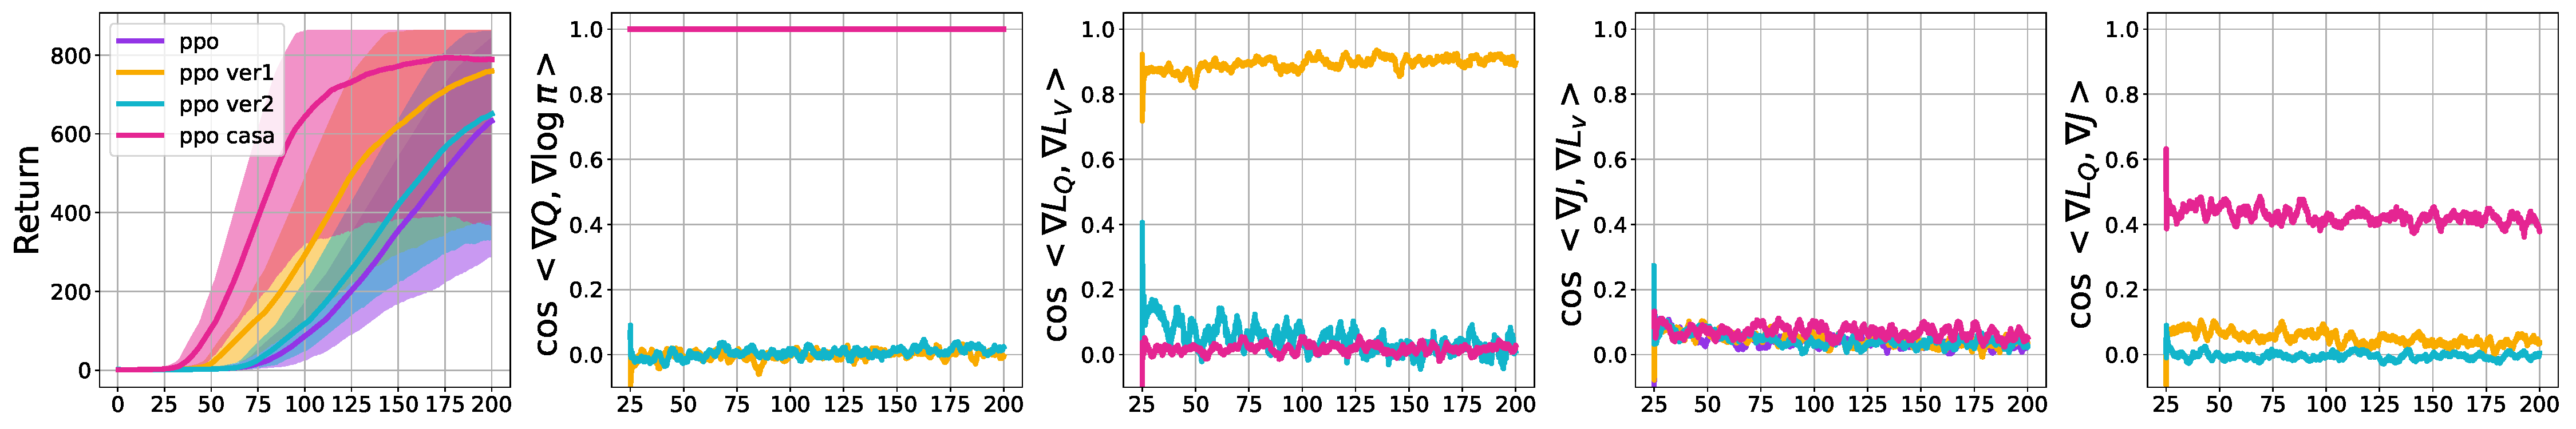
\includegraphics[width=\linewidth]{body/app_fig/app_ppo_Breakout.pdf}

% 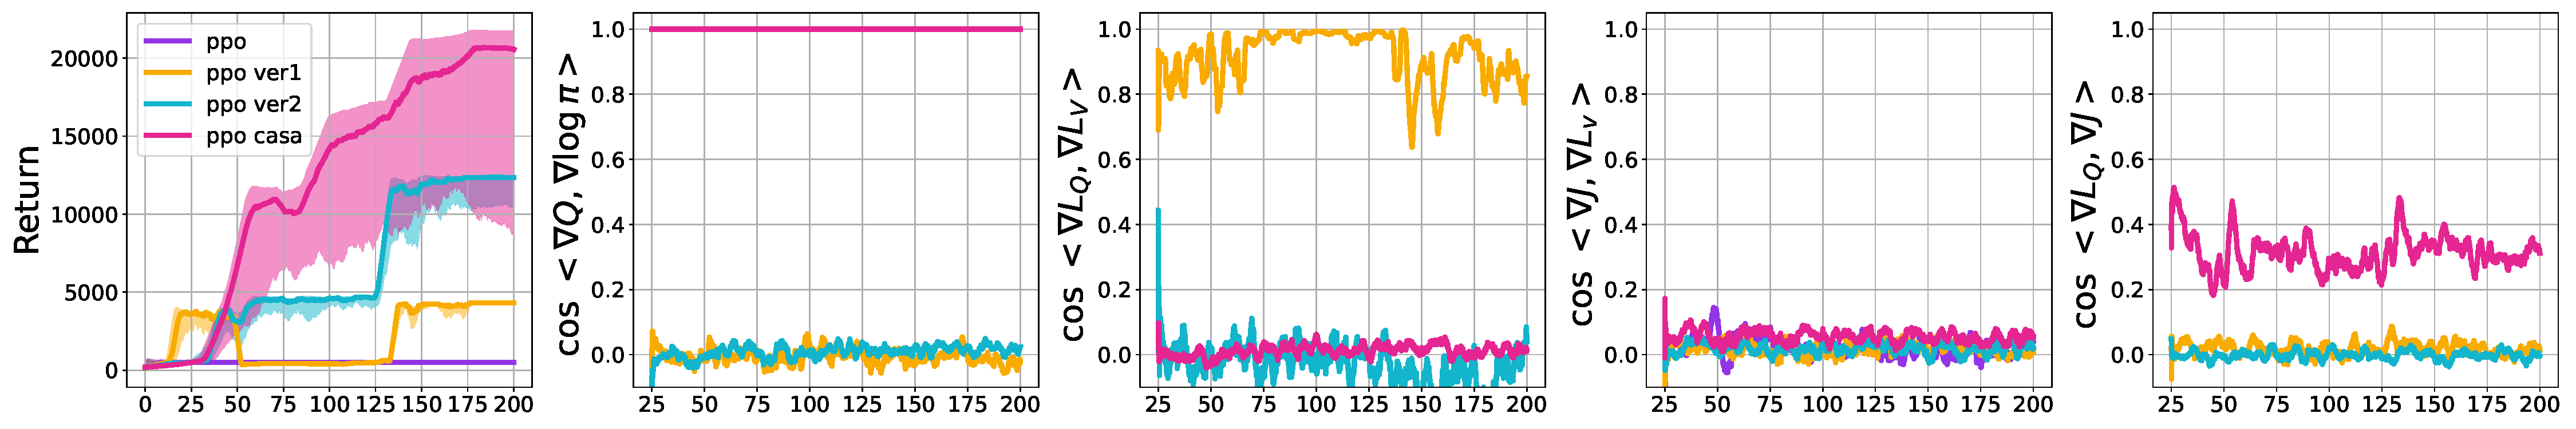
\includegraphics[width=\linewidth]{body/app_fig/app_ppo_Qbert.pdf}

% 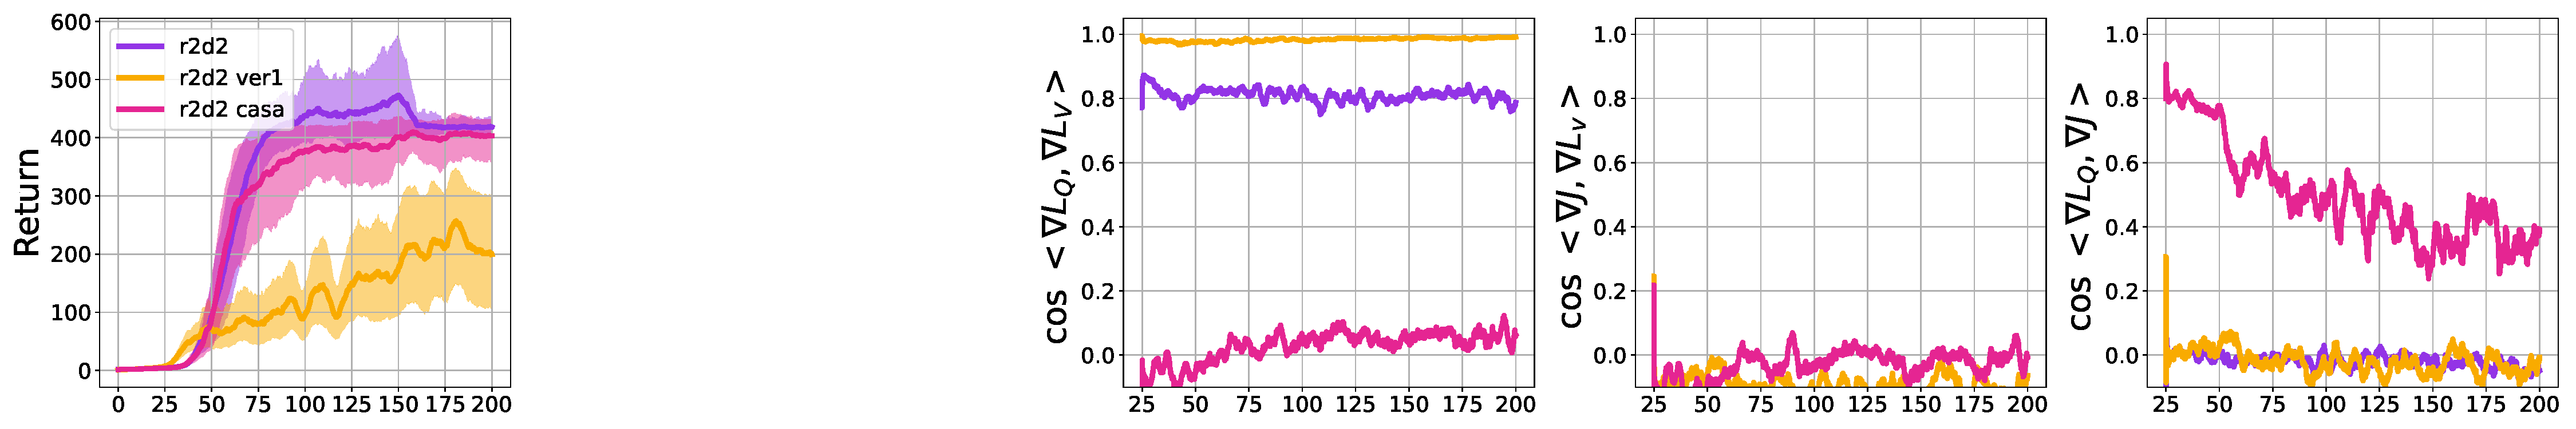
\includegraphics[width=\linewidth]{body/app_fig/app_r2d2_Breakout.pdf}


% 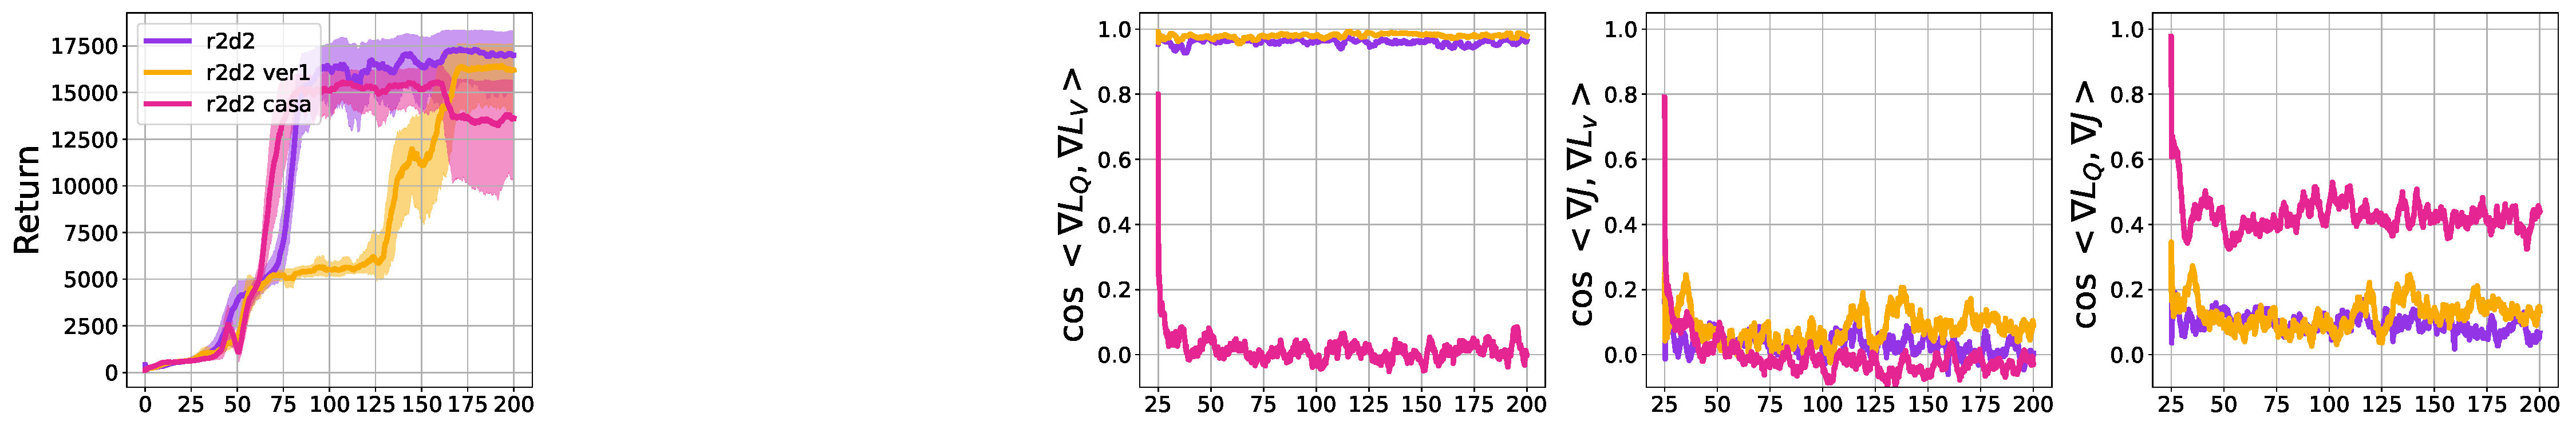
\includegraphics[width=\linewidth]{body/app_fig/app_r2d2_Qbert.pdf}
% \caption{Angles of Gradients and Returns of versions of PPO and R2D2 defined in Table \ref{tab:ppo_mtv} and Table \ref{tab:r2d2_mtv}.}
% \label{fig:mtv_app}
% \end{figure}

% \clearpage

% \changnan{casa summary deleted}
% \section{CASA summary}
% \begin{figure}[ht]
% \centering
% 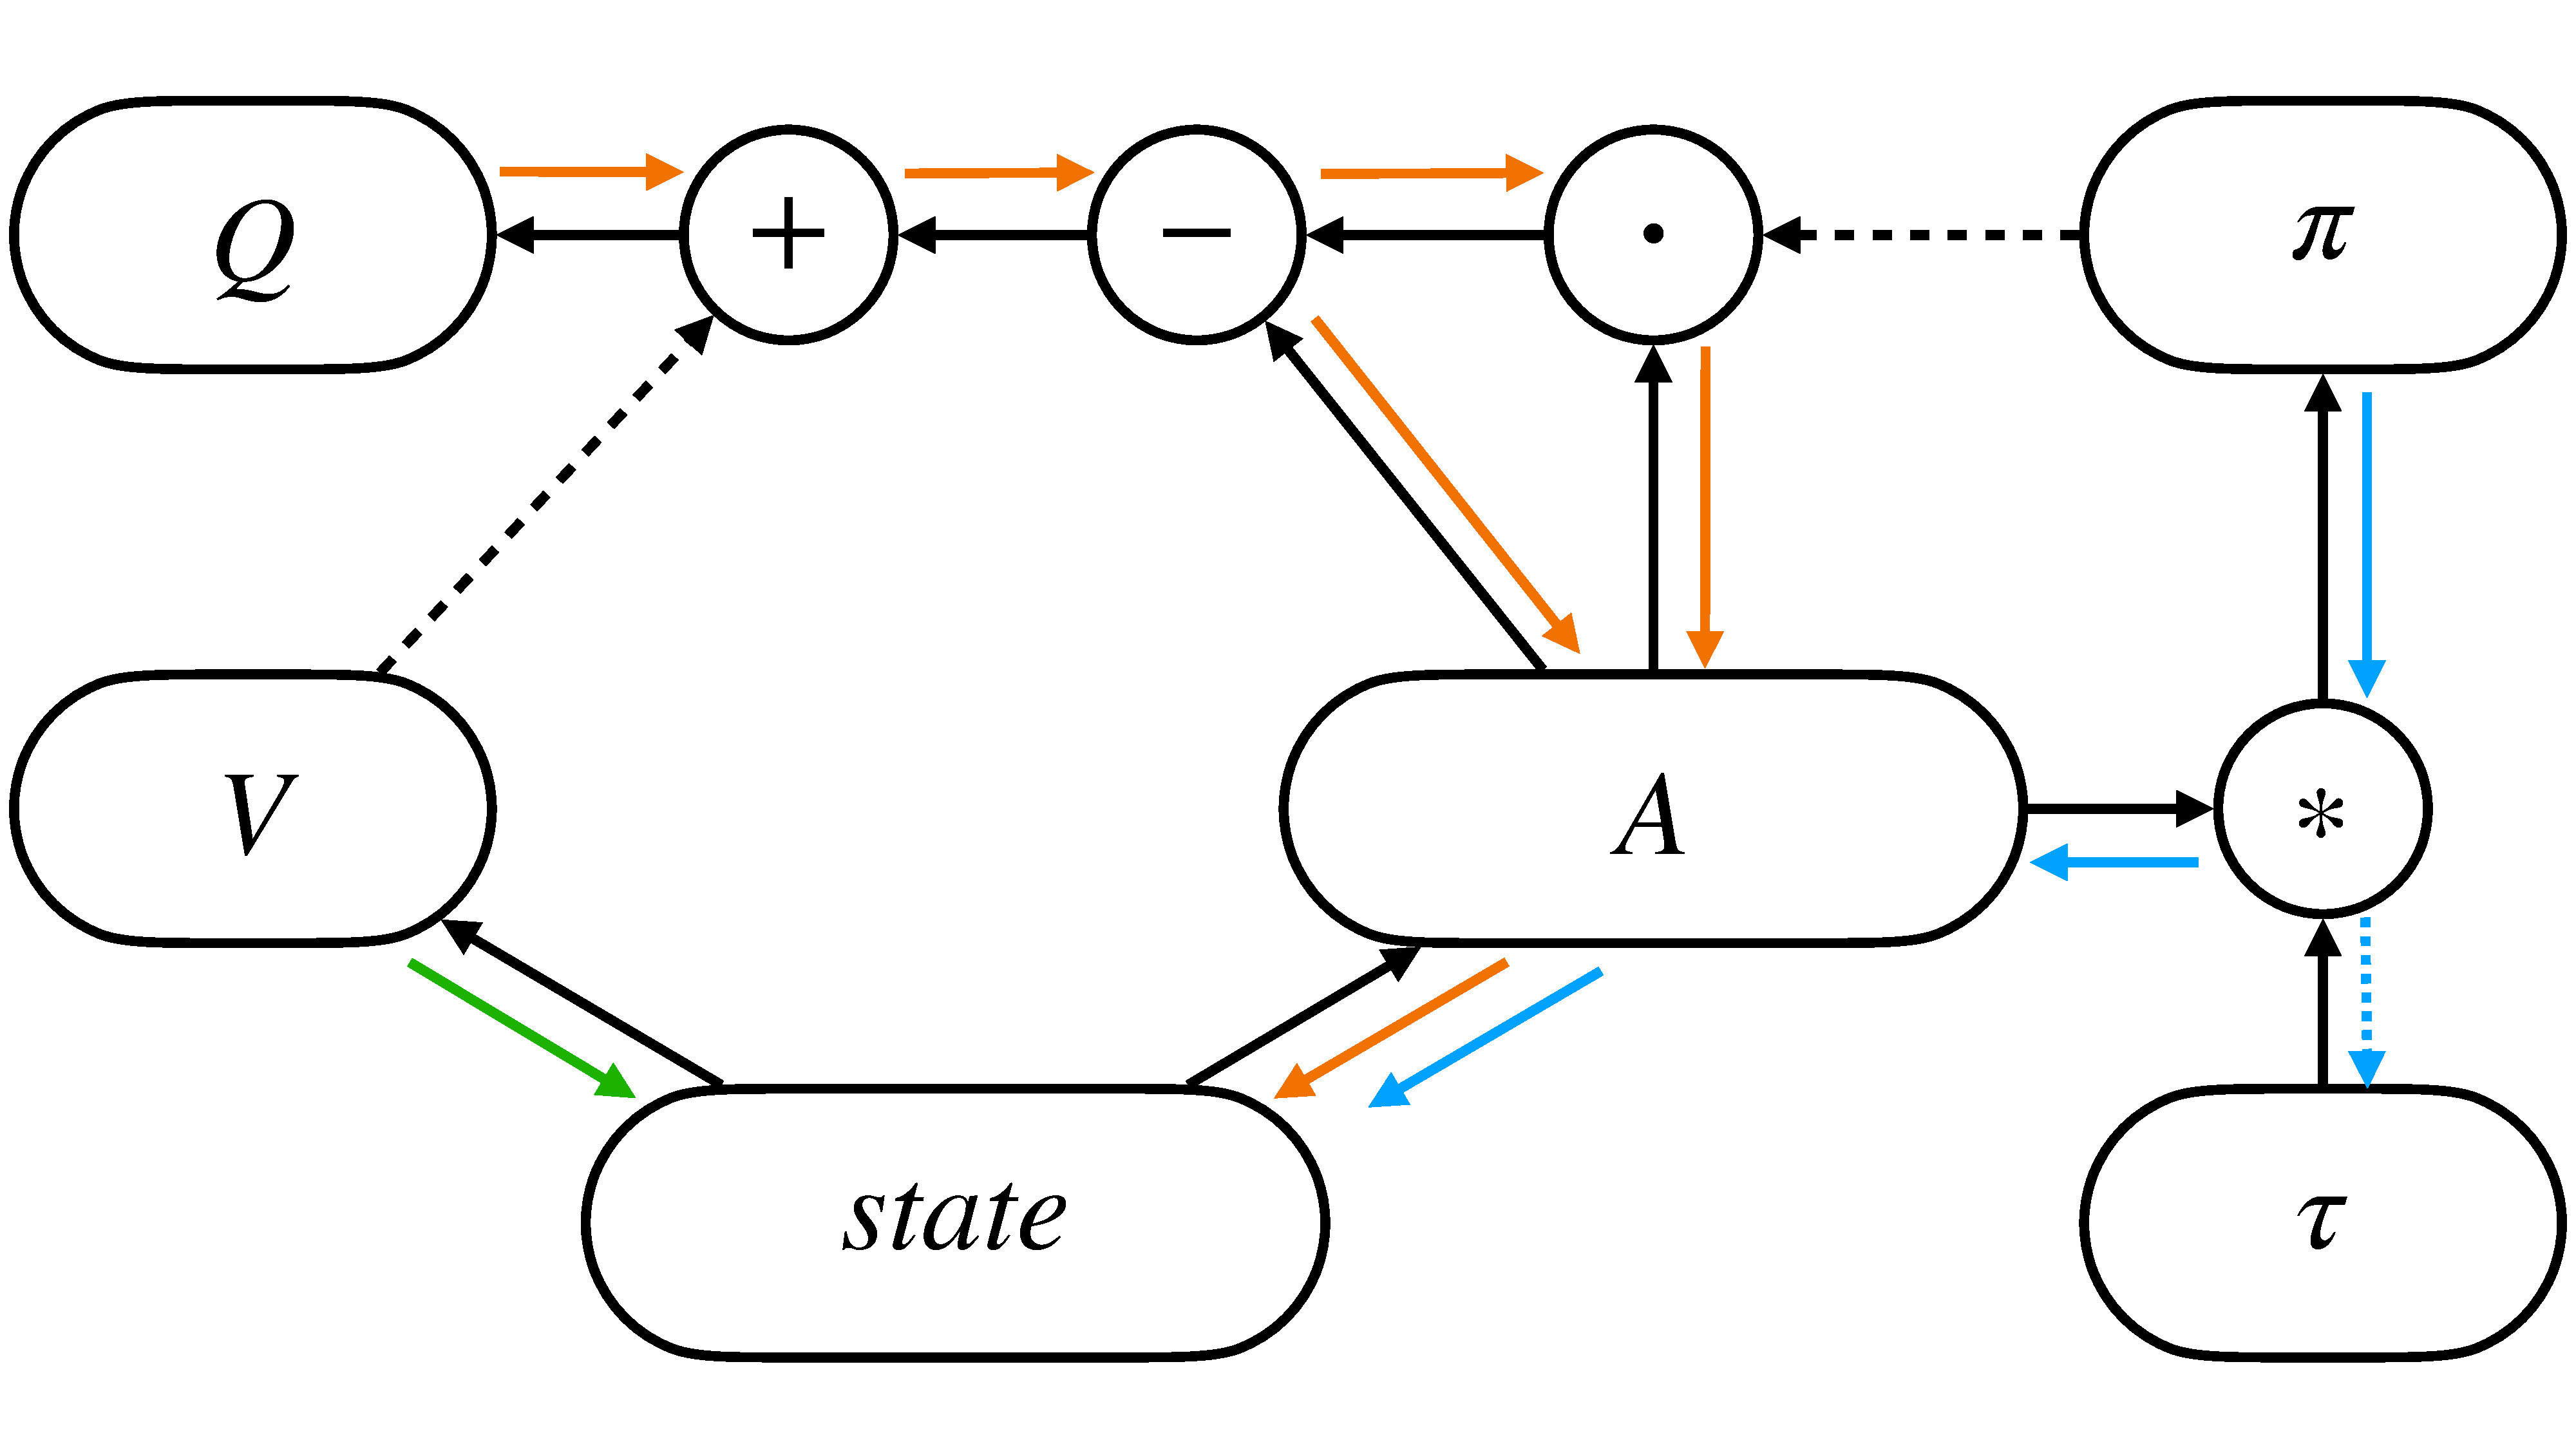
\includegraphics[width=0.4\textwidth,bb= 0 0 1800 1100]{body/figures/CASA.pdf}
% \caption{
% \textbf{Black} lines represent the forward process.
% \textbf{Dotted} black lines represent the \textit{stop gradient} operator in the forward process. 
% \textbf{Colorful} lines represent backpropagation from different loss functions. 
% Specifically, \textbf{blue} lines represent $\mathbb{E}_\pi [(Q^\pi-V)\nabla \log \pi]$, 
% \textbf{orange} lines represent $\mathbb{E}_\pi [(Q^\pi-Q)\nabla Q]$,
% and \textbf{green} lines represent $\mathbb{E}_\pi [(Q^\pi-V)\nabla V]$.}
% \label{fig:casa}
% \end{figure}
% \section{motivation experiments}

\clearpage

{\colorred \section{On Discussing Application of CASA on Continuous Action Space}
\label{app:cts_space}

As we can see CASA is only applied to discrete action space in the main context, we make a discussion on whether CASA is applicable on continuous action space. 
For brevity, we let $\tau=1$ and write \eqref{eq:casa} as:
\begin{equation}
\left\{
    \begin{aligned}
        &\pi = \text{softmax}(A), \\
        &\Bar{A} = A - \mathbb{E}_{\pi} [A], \\
        &Q = \Bar{A} + sg(V).
    \end{aligned}
\right. 
\end{equation}
The difficulty comes from estimating two quantities, one is $\text{softmax}(A)$, the other is $\mathbb{E}_{\pi} [A]$. 
This comes from the fact that discrete action space is countable so these two quantities are expressed in a closed-form, while continuous action space is uncountable so an accurate estimation of these two quantities is intractable. 
We can surely apply Monte Carlo methods to approximate, but a more elegant close-form expression may be preferred. 
Then this becomes another problem: \textit{how to estimate (state-action values / advantages / policy probabilities) of all actions in a continuous action space efficiently without loss of generality?}
This is another representational design problem, which is out of scope of this paper, so we don't touch much about it. 
But with the hope of inspiring a better solution to this problem, we provide one practical way of applying CASA on continuous action space based on kernel-based machine learning. 

Let $a_0, \dots, a_k$ to be basis actions in the action space. 
Let $A(s, a_0), \dots, A(s, a_k)$ to be advantage functions for tuples of states and basis actions. 
They can either share parameters or be isolated. 
Let $K(\cdot, \cdot)$ be a kernel function defined on the product of two action spaces. 
For any $a$ in the action space, we can estimate $A(s, a)$ by a decomposition such like $$A(s, a) = \frac{1}{Z_a} (K(a_0, a) A(s, a_0) + \dots + K(a_k, a) A(s, a_k)),$$ where $Z_a = \sum_{i=0}^k K(a_i, a)$ is a normalization constant. 

Since $K(\cdot, a)$ is a closed-form function of $a$, and $|\{A(s, a_0), \dots, A(s, a_k)\}|$ is finite, we can make a closed-form expression of both $\text{softmax}(A)$ and $\mathbb{E}_{\pi} [A]$. 
Then we can apply CASA directly on this expression, with one function estimates $V$ and the other function estimates advantages of all actions in a closed-form with only state as input.  
The policy is defined directly by $\text{softmax}$ of all advantages. 
In details, we define
\begin{equation}
\left\{
    \begin{aligned}
        &\pi(s, a) = \exp (A(s, a)) / \int_{a} \exp (A(s, a)) da, \\
        &\Bar{A}(s, a) = A(s, a) - \int_{a} sg(\pi(s, a)) A(s, a) da, \\
        &Q(s, a) = \Bar{A}(s, a) + sg(V(s)).
    \end{aligned}
\right. 
\end{equation}

Then it satisfies the consistency of CASA on continuous action space.
$$
\begin{aligned}
    \nabla \log \pi(s, a) &= \nabla A(s, a) - \frac{\nabla \int_{a} \exp (A(s, a)) da}{\int_{a} \exp (A(s, a)) da} \\
    &= \nabla A(s, a) - \frac{ \int_{a} \exp (A(s, a)) \nabla A(s, a) da}{\int_{a} \exp (A(s, a)) da} \\
    &= \nabla A(s, a) - \int_{a} \frac{  \exp (A(s, a)) }{\int_{a} \exp (A(s, a)) da} \nabla A(s, a) da \\
    &= \nabla A(s, a) - \int_{a} \pi(s, a) \nabla A(s, a) da \\
    &= \nabla \Bar{A}(s, a) = \nabla Q(s, a). 
\end{aligned}
$$
}

\section{DR-Trace}
\label{app:drtrace}

% One simple choice is to learn $V$ and $\pi$ by V-Trace \citep{impala} and to learn $Q$ by ReTrace \citep{retrace}. 
% \citep{impala} shows that $V^{\Tilde{\pi}}$ estimated by V-Trace converges to $V^*$ that corresponds to some $\Tilde{\pi}_{VTrace}$.
% Respectively, \citep{retrace} shows that $Q^{\Tilde{\pi}}$ estimated by ReTrace converges to $Q^*$ that corresponds to some $\Tilde{\pi}_{ReTrace}$.

As CASA estimates $(V, Q, \pi)$, we would ask
\textbf{i)} how to guarantee that $\Tilde{\pi}_{VTrace} = \Tilde{\pi}_{ReTrace}$, 
\textbf{ii)} how to exploit $(V, Q, \pi)$ to make a better estimation. 
Though we can apply V-Trace to estimate $V$ and ReTrace to estimate $Q$ with proper hyperparameters to guarantee $\Tilde{\pi}_{VTrace} = \Tilde{\pi}_{ReTrace}$, it's more reasonable to estimate $(V, Q)$ together. 
Inspired by Doubly Robust, which is shown to maximally reduce the variance, we introduce DR-Trace, which estimates $V$ by 
$$
\label{eq:dr-v}
    \begin{aligned}
        V_{DR}^{\Tilde{\pi}} (s_t) &\overset{def}{=} \mathbb{E}_{\mu} [ 
        V(s_t) + \sum_{k \geq 0} \gamma^k 
     c_{[t:t+k-1]} \rho_{t+k}  \delta^{DR}_{t+k} ],  
    \end{aligned}
$$
{\colorred where $\mu$ is the behavior policy}, $\delta^{DR}_t \overset{def}{=} r_t + \gamma V(s_{t+1}) - Q(s_t, a_t)$ is one-step Doubly Robust error, $\rho_t \overset{def}{=} \min\{\frac{\pi_t}{\mu_t}, \Bar{\rho} \}$ and $c_t \overset{def}{=} \min\{\frac{\pi_t}{\mu_t}, \Bar{c}\}$ are clipped per-step importance sampling, $c_{[t: t+k]} \overset{def}{=} \prod_{i=0}^{k} c_{t+i}$.

With one step Bellman equation, we estimate $Q$ by
$$
\label{eq:dr-q}
    \begin{aligned}
         Q_{DR}^{\Tilde{\pi}} (s_t, a_t) 
         &\overset{def}{=} \mathbb{E}_{s_{t+1}, r_t \sim p(\cdot, \cdot | s_t, a_t)} [  r_t + \gamma   V_{DR}^{\Tilde{\pi}} (s_{t+1}) ] 
        \\
        %  &=  \mathbb{E}_{\mu} [ r_t + \gamma V(s_{t + 1}) +
        % \gamma \sum_{k \geq 0} \gamma^k 
        % c_{[t+1:t+k]} \rho_{t+1+k}
        % \delta^{DR}_{t+1+k} V
        % ]
        % \\
        %  &= \mathbb{E}_{\mu}   [
        % Q(s_t, a_t) + \delta_t^{DR}V + \sum_{k \geq 1}  \gamma^k
        % c_{[t+1:t+k-1]} \rho_{t+k}
        % \delta^{DR}_{t+k} V
        % ],
        % \\
        &=  \mathbb{E}_{\mu}   [
        Q(s_t, a_t) + \sum_{k \geq 0}  \gamma^k
        c_{[t+1:t+k-1]} \Tilde{\rho}_{t, k}
        \delta^{DR}_{t+k}
        ], 
    \end{aligned}
$$
where $\Tilde{\rho}_{t, k} =  1_{\{k=0\}} + 1_{\{k > 0\}} \rho_{t+k}$.

% Compared to \eqref{eq:dr-v}, $c_{[t+1:t+k-1]} \Tilde{\rho}_{t, k}$ in \eqref{eq:dr-q} doesn't multiply importance sampling ratio of $a_t$, which meets the same intuition as \eqref{eq:vtrace} and \eqref{eq:retrace}.\\
\begin{theorem}
    Define $\Bar{A} = A - \mathbb{E}_\pi[A]$, $Q = \Bar{A} + sg(V)$,
    $$
    \begin{aligned}
    &\mathscr{T}(Q) \overset{def}{=} \mathbb{E}_{\mu}   [
        Q(s_t, a_t) + \sum_{k \geq 0}  \gamma^k
        c_{[t+1:t+k-1]} \Tilde{\rho}_{t, k}
        \delta^{DR}_{t+k}
        ], \\
    &\mathscr{S}(V) \overset{def}{=} \mathbb{E}_{\mu}   [
        V(s_t) + \sum_{k \geq 0}  \gamma^k
        c_{[t:t+k-1]} \rho_{t, k}
        \delta^{DR}_{t+k}
        ], \\
    &\mathscr{U}(Q, V) = (\mathscr{T}(Q) - \mathbb{E}_\pi[Q] + \mathscr{S}(V), \mathscr{S}(V)), \\
    &\mathscr{U}^{(n)}(Q, V) = \mathscr{U}(\mathscr{U}^{(n-1)}(Q, V)),
    \end{aligned}
    $$
    then $\mathscr{U}^{(n)}(Q, V) \rightarrow (Q^{\Tilde{\pi}}, V^{\Tilde{\pi}})$ that corresponds to 
    $$
        \Tilde{\pi}(a|s) = \frac
        {\min \left\{\Bar{\rho} \mu (a|s), \pi(a|s)\right\}}
        {\sum_{b \in \mathcal{A}}\min \left\{\Bar{\rho} \mu (b|s), \pi(b|s)\right\}}.
    $$ as $n \rightarrow +\infty$.
\label{thm:dr}
\end{theorem}
\begin{proof}
    See Appendix \ref{app:proof}, Theorem \ref{thm_app:dr}.
\end{proof}
Theorem \ref{thm:dr} shows that DR-Trace is a contraction mapping and $(V, Q)$ converges to $(V^{\Tilde{\pi}}, Q^{\Tilde{\pi}})$ that corresponds to 
$$
    \begin{aligned}
        \Tilde{\pi}(a|s) = \frac
        {\min \left\{\Bar{\rho} \mu (a|s), \pi(a|s)\right\}}
        {\sum_{b \in \mathcal{A}}\min \left\{\Bar{\rho} \mu (b|s), \pi(b|s)\right\}}.
    \end{aligned}
$$

% At training time, the policy evaluation is achieved by updating $\theta$ to minimize $l2$ losses
% $$
% \begin{aligned}
%     L_V(\theta) &= \mathbb{E}_\pi [ (V_\theta(s_t) -  V_{DR}^{\Tilde{\pi}} (s_t))^2 ], \\
%     L_Q(\theta) &= \mathbb{E}_\pi [ (Q_\theta(s_t, a_t) -  Q_{DR}^{\Tilde{\pi}} (s_t, a_t))^2 ],
% \end{aligned}
% $$ 
% which gives the ascent direction of $\theta$ by
% \begin{equation}
% \label{eq:grad_qv}
%     \begin{aligned}
%         \nabla_\theta L_V(\theta)
%         &= \mathbb{E}_\pi \left[ (V_{DR}^{\Tilde{\pi}} (s_t) - V_\theta(s_t) ) \nabla V_\theta(s_t) \right], \\
%         \nabla_\theta L_Q(\theta)
%         &= \mathbb{E}_\pi \left[ (Q_{DR}^{\Tilde{\pi}} (s_t, a_t) - Q_\theta(s_t, a_t)) \nabla Q_\theta(s_t, a_t) \right].
%     \end{aligned}
% \end{equation}
% And we make the policy improvement by policy gradient, which gives the ascent direction of $\theta$ by 
% \begin{equation}
% \label{eq:grad_pi}
% \begin{aligned}
%     \nabla_\theta \mathcal{J}(\tau, \theta) = \mathbb{E}_\mu \left[\tau \rho_t (Q_{DR}^{\Tilde{\pi}} (s_t, a_t) - V_\theta(s_t) ) \nabla_\theta \log \pi_t \right],
% \end{aligned}
% \end{equation}
% where $\mathcal{J} (\tau, \theta) = \tau \mathbb{E}_\pi [\sum \gamma^t r_t]$.
% It takes an additional $\tau$, which frees the scale of gradient from $\tau$.

% Finally, the gradient ascent direction of $\theta$ is given by
% \begin{equation}
%     \label{eq:grad_all}
%     \alpha_1 \nabla_\theta L_V + \alpha_2 \nabla_\theta L_Q + \alpha_3 \nabla_\theta \mathcal{J}.
% \end{equation}

% \textbf{Full algorithm is described in Appendix \ref{app:casa}.}
% Note that \eqref{eq:grad_all} doesn't need any entropy regularization. 
% We will discuss why this happens in section \ref{sec:equiv} and how CASA controls the exploration in section \ref{sec:ent_control}.


\begin{figure}[h]
    \centering
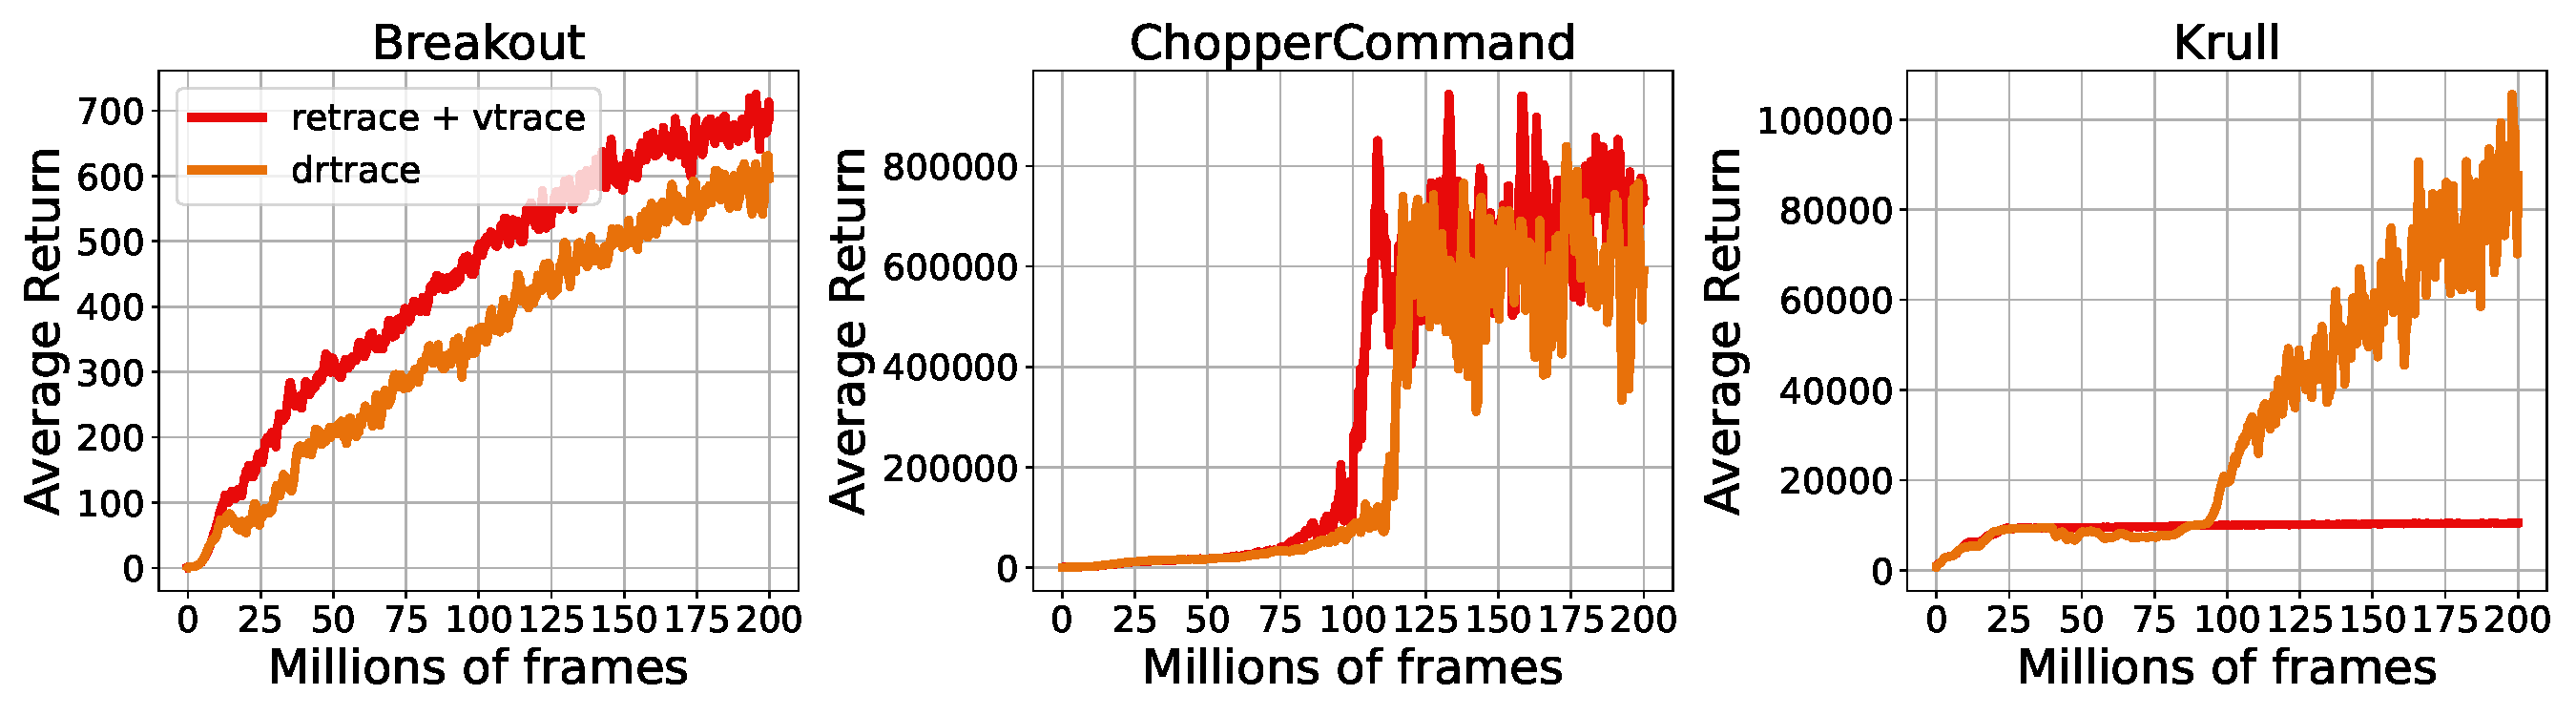
\includegraphics[width=\linewidth]{body/ablation/dr_ablation.pdf}
    \caption{Ablation study for w/wo DR-Trace on Breakout, ChopperCommand and Krull.}
    \label{fig:app_dr_trace}
\end{figure}

According to our proof, DR-Trace should work similar to V-Trace and ReTrace, as the convergence rate and the limitation are same. 
We compare DR-Trace with V-Trace+ReTrace in Figure \ref{fig:app_dr_trace}, where we replace estimation of state values by V-Trace and estimation of state-action values by ReTrace. 
We call V-Trace+ReTrace as No-DR-Trace for brevity. 
No-DR-Trace performs better on Breakout and ChopperCommand, but fails to make a breakthrough on Krull. 
Recalling the fact that Doubly Robust can maximally reduce the variance of Bellman error, No-DR-Trace is less stable but also potential to achieve a better performance. 
A conclusion cannot be made about No-DR-Trace, as this phenomenon means that No-DR-Trace is less stable than DR-Trace, but it also holds the potential to achieve a better performance.

% \clearpage


\section{Proofs}
\label{app:proof}

\theoremstyle{plain}
% \setcounter{Lemma}{0}
\newtheorem{Lemma_app}{Lemma}[section]
\newtheorem{Theorem_app}{Theorem}[section]
\theoremstyle{definition}
\newtheorem*{Remark_app}{Remark}
\theoremstyle{remark}

% \begin{Lemma_app}
% Let 
% $g \in \textbf{C}^{1}(\mathbb{R}^{n}): \mathbb{R}^{n} \to \mathbb{R}^{n}, \ f \in \textbf{C}^{1}(\mathbb{R}^{n+k}): \mathbb{R}^{n+k} \to \mathbb{R}^{n}.
% $\\
% If
% $
% \nabla_x g(x) = \nabla_x f(x, y)$, for $\forall x\in \mathbb{R}^{n}, y\in \mathbb{R}^k,
% $
% then $\exists$ $c \in \textbf{C}^{1}(\mathbb{R}^{k}): \mathbb{R}^{k} \to \mathbb{R}^{n}$, s.t. $f(x, y) = g(x) + c(y)$.
% \label{lemma_app:func_sep}
% \end{Lemma_app}
% \begin{proof}

% Let $\Tilde{f}(x, y) = f(x, y) - g(x)$.

% Since $\nabla_x g(x) = \nabla_x f(x, y)$, we have 
% $$
% \nabla_x \Tilde{f} = 0, \ for \ \forall x\in \mathbb{R}^{n}, y\in \mathbb{R}^k.
% $$

% So $\Tilde{f}$ is a constant function w.r.t $x$, which can be denoted as $c(y) = \Tilde{f}(x, y)$.

% Hence, $f(x, y) = g(x) + c(y)$.
% \end{proof}

\begin{Lemma_app}
(i) Define $\pi = softmax(A / \tau)$, then $\nabla \log \pi = (\textbf{1} - \pi) \frac{\nabla A}{\tau}$. 
(ii) Denote $sg$ to be stop gradient and define $\Bar{A} = A - \mathbb{E}_\pi [A]$, $Q = \Bar{A} + sg(V)$, then $\nabla Q = (\textbf{1} - \pi) \nabla A$.
\label{lemma_app:vannila_grad}
\end{Lemma_app}
\begin{proof}

As $Q = \Bar{A} + sg(V) = A - sg(\pi)\cdot A + sg(V)$, it's obvious that $\nabla Q = (\textbf{1} - \pi) \nabla A$.

For $\log \pi$, it's a standard derivative of cross entropy, so we have $\nabla \log \pi = (\textbf{1} - \pi) \nabla (A / \tau) = (\textbf{1} - \pi) \frac{\nabla A}{\tau}$.
\end{proof}

\begin{Lemma_app}
Define $\Bar{A}= A - \mathbb{E}_\pi[A]$, $Q = \Bar{A} + sg(V), \pi = softmax(A / \tau)$, then 
$$
\mathbb{E}_\pi \left[ (Q - V) \nabla \log \pi \right]
= - \tau \nabla \textbf{H}[\pi].
$$
\label{lemma_app:eqiv_pg_ent}
\end{Lemma_app}
\begin{proof}
Since 
$$
\pi = \exp(A / \tau) / Z,\ Z = \int_\mathcal{A} \exp(A / \tau),
$$
we have 
$$
A = \tau \log \pi + \tau \log Z.
$$
Based on the observation that $\mathbb{E}_\pi \left[ f(s) \nabla \log \pi (\cdot | s) \right] = 0$, 
we have 
$$\mathbb{E}_\pi \left[ \mathbb{E}_\pi[A] \cdot \nabla \log \pi \right] = 0,$$ 
$$\mathbb{E}_\pi \left[ \log Z \cdot \nabla \log \pi \right] = 0.$$

On the one hand,
$$
\begin{aligned}
    \mathbb{E}_\pi \left[ (Q - V) \nabla \log \pi \right]
    &= \mathbb{E}_\pi \left[ A \nabla \log \pi \right] 
    - \mathbb{E}_\pi \left[ \mathbb{E}_\pi[A] \cdot \nabla \log \pi \right] \\
    &= \tau \mathbb{E}_\pi \left[ \log \pi \nabla \log \pi \right]
    + \tau \mathbb{E}_\pi \left[ \log Z \cdot \nabla \log \pi \right] \\
    &= \tau \mathbb{E}_\pi \left[ \log \pi \nabla \log \pi \right].
\end{aligned}
$$

On the other hand, 
$$
\begin{aligned}
    \nabla \textbf{H} [\pi] 
    &= - \nabla \int_\mathcal{A} \pi_i \log \pi_i \\
    &= - \int_\mathcal{A}  \nabla \pi_i \cdot \log \pi_i - \int_\mathcal{A} \pi_i \nabla \log \pi_i  \\
    &= - \int_\mathcal{A}  \pi_i \nabla \log \pi_i \cdot \log \pi_i - \int_\mathcal{A}  \pi_i \frac{\nabla \pi_i}{\pi_i} \\
    &= - \mathbb{E}_\pi \left[ \log \pi \nabla \log \pi \right].
\end{aligned}
$$
Hence, $
\mathbb{E}_\pi \left[ (Q - V) \nabla \log \pi \right]
= - \tau \nabla \textbf{H}[\pi]
$.
\end{proof}

\begin{Theorem_app}
    Define $\Bar{A} = A - \mathbb{E}_\pi[A]$, $Q = \Bar{A} + sg(V)$.
    Define $$
    \begin{aligned}
    &\mathscr{T}(Q) \overset{def}{=} \mathbb{E}_{\mu}   [
        Q(s_t, a_t) + \sum_{k \geq 0}  \gamma^k
        c_{[t+1:t+k-1]} \Tilde{\rho}_{t, k}
        \delta^{DR}_{t+k}
        ], \\
    &\mathscr{S}(V) \overset{def}{=} \mathbb{E}_{\mu}   [
        V(s_t) + \sum_{k \geq 0}  \gamma^k
        c_{[t:t+k-1]} \rho_{t, k}
        \delta^{DR}_{t+k}
        ], \\
    &\mathscr{U}(Q, V) = (\mathscr{T}(Q) - \mathbb{E}_\pi[Q] + \mathscr{S}(V), \mathscr{S}(V)), \\
    &\mathscr{U}^{(n)}(Q, V) = \mathscr{U}(\mathscr{U}^{(n-1)}(Q, V)),
    \end{aligned}
    $$
    then $\mathscr{U}^{(n)}(Q, V) \rightarrow (Q^{\Tilde{\pi}}, V^{\Tilde{\pi}})$ that corresponds to 
    $$
        \Tilde{\pi}(a|s) = \frac
        {\min \left\{\Bar{\rho} \mu (a|s), \pi(a|s)\right\}}
        {\sum_{b \in \mathcal{A}}\min \left\{\Bar{\rho} \mu (b|s), \pi(b|s)\right\}}.
    $$ as $n \rightarrow +\infty$.
\label{thm_app:dr}
\end{Theorem_app}
\begin{Remark_app}
$\mathscr{T}(Q) - \mathbb{E}_\pi[Q] + \mathscr{S}(V)$ is \textbf{exactly} how $Q$ is updated at training time. 
Since $Q = \Bar{A} + sg(V)$, if we apply gradient ascent on $Q$ and $V$ in directions $\nabla L_Q(\theta)$ and $\nabla L_V(\theta)$ respectively, change of $Q$ comes from two aspects. One comes from $\nabla L_Q(\theta)$, which changes $A$, the other comes from $\nabla L_V(\theta)$, which changes $V$. Because the gradient of $V$ is stopped when estimating $Q$, the latter is captured by "minus old baseline, add new baseline", which is $- \mathbb{E}_\pi[Q] + \mathscr{S}(V)$ in Theorem \ref{thm_app:dr}.
\end{Remark_app}
\begin{proof}
 Define
 $$
 \begin{aligned}
        \widetilde{\mathscr{T}}(Q) &= - \mathbb{E}_\pi[Q] + \mathscr{T}(Q), \\
        \widetilde{\mathscr{U}}(Q, V) &= (\widetilde{\mathscr{T}}(Q), \mathscr{S}(V)), \\
        \widetilde{\mathscr{U}}^{(n)}(Q, V) &=   \widetilde{\mathscr{U}}(\widetilde{\mathscr{U}}^{(n-1)}(Q, V)).
 \end{aligned}
 $$
By Lemma \ref{lemma_app:dr_q}, $\widetilde{\mathscr{T}}^{(n)}(Q)$ converges to some $A^*$ as $n \rightarrow \infty$. This process will not influence the estimation of $V$ as the gradient of $V$ is stopped when estimating $Q$. According to the proof, $A^*$ does not depend on $V$. \\
By Lemma \ref{lemma_app:dr_v}, $\mathscr{S}^{(n)}(V)$ converges to some $V^*$ as $n \rightarrow \infty$. \\
Hence, we have
$$
\widetilde{\mathscr{U}}^{(n)}(Q, V) \rightarrow (A^*, V^*)\ \ as\ \ n \rightarrow +\infty. 
$$
By definition, 
$$
\mathscr{U}(Q, V) = (\widetilde{\mathscr{T}}(Q) + \mathscr{S}(V), \mathscr{S}(V)),
$$
we can regard $\widetilde{\mathscr{T}}(Q) + \mathscr{S}(V)$ as $Q$ and regard $\mathscr{S}(V)$ as $V$, then
$$
\begin{aligned}
    \mathscr{U}^{(2)}(Q, V) 
    &= \mathscr{U}(\widetilde{\mathscr{T}}(Q) + \mathscr{S}(V), \mathscr{S}(V)) \\
    &= (\mathscr{T}(\widetilde{\mathscr{T}}(Q) + \mathscr{S}(V)) -\mathscr{S}(V) + \mathscr{S}^{(2)}(V), \mathscr{S}^{(2)}(V)) \\
    &= (\widetilde{\mathscr{T}}^{(2)}(Q) + \mathscr{S}^{(2)}(V), \mathscr{S}^{(2)}(V)).
\end{aligned}
$$
By induction, 
$$
\begin{aligned}
    \mathscr{U}^{(n)}(Q, V) &= (\widetilde{\mathscr{T}}^{(n)}(Q) + \mathscr{S}^{(n)}(V), \mathscr{S}^{(n)}(V)) \\
    &\rightarrow (A^*+V^*, V^*)\ \ as\ \ n\rightarrow + \infty.
\end{aligned}
$$
Same as \citep{impala}, 
$$
    \Tilde{\pi}(a|s) = \frac
    {\min \left\{\Bar{\rho} \mu (a|s), \pi(a|s)\right\}}
    {\sum_{b \in \mathcal{A}}\min \left\{\Bar{\rho} \mu (b|s), \pi(b|s)\right\}}.
$$ 
is the policy s.t. the Bellman equation holds, which is 
$$\mathbb{E}_\mu[\rho_t (r_t + \gamma V_{t+1} - V_t) | \mathscr{F}_t] = 0,$$ and $\mathscr{U}(Q^{\Tilde{\pi}}, V^{\Tilde{\pi}}) = (Q^{\Tilde{\pi}}, V^{\Tilde{\pi}})$. \\
So we have
$(A^*+V^*, V^*) = (Q^{\Tilde{\pi}}, V^{\Tilde{\pi}}).$
\end{proof}

\begin{Lemma_app}
Define $\Bar{A}= A - \mathbb{E}_\pi[A]$, $Q = \Bar{A} + sg(V)$,
then operator 
$$
    \mathscr{T}(Q) \overset{def}{=} \mathbb{E}_{\mu}   [
        Q(s_t, a_t) + \sum_{k \geq 0}  \gamma^k
        c_{[t+1:t+k-1]} \Tilde{\rho}_{t, k}
        \delta^{DR}_{t+k}
        ]
$$
is a contraction mapping w.r.t. $Q$.
\label{lemma_app:dr_q}
\end{Lemma_app}
\begin{Remark_app}
Note that $\mathscr{T}(Q)$ is exactly \eqref{eq:dr-q}. 

Since $Q = A + sg(V)$, the gradient of $V$ is stopped when estimating $Q$, updating $Q$ will not change $V$, which is equivalent to updating $A$.
Without loss of generality, we assume $V$ is fixed as $V^*$ in the proof.
\end{Remark_app}
\begin{proof}

$\Bar{A} = A - \mathbb{E}_\pi[A]$ shows $\mathbb{E}_\pi[\Bar{A}] = 0$, which guarantees that no matter how we update $A$, we always have $\mathbb{E}_\pi[Q] = V^*$.

Based on above observations, define 
$$
    \widetilde{\mathscr{T}}(Q) \overset{def}{=} - \mathbb{E}_\pi [Q] + \mathscr{T}(Q).
$$

It's obvious that we only need to prove $\widetilde{\mathscr{T}}(Q)$ is a contraction mapping.

For brevity, we denote $$Q_t = Q(s_t, a_t), A_t = A(s_t, a_t), V^*_t = V^*(s_t).$$

Noticing that $\Tilde{\rho}_{t, 0} = 1$, let $\mathscr{F}$ represent filtration, we can rewrite $\widetilde{\mathscr{T}}$ as 
\begin{equation}
\label{eq:dr_a_2}
\begin{aligned}
    \widetilde{\mathscr{T}}(Q)
    &= \mathbb{E}_{\mu}   [
        A_t + \sum_{k \geq 0}  \gamma^k
        c_{[t+1:t+k-1]} \Tilde{\rho}_{t, k}
        \delta^{DR}_{t+k}
        ] \\
    &= \mathbb{E}_{\mu}   [
        -V^*_t + \sum_{k \geq 0}  \gamma^k
        c_{[t+1:t+k-1]} \Tilde{\rho}_{t, k}
        r_{t+k}
        + 
        \sum_{k \geq 0}  \gamma^{k+1}
        c_{[t+1:t+k-1]} \Delta_k ],
        \\
\end{aligned}
\end{equation}
where 
\begin{equation}
\label{eq:dr_delta}
    \Delta_k = \mathbb{E}_{\mu}\left[\Tilde{\rho}_{t, k} V^*_{t+k+1} - c_{t+k} \Tilde{\rho}_{t, k+1} Q_{t+k+1} | \mathscr{F}_{t+k}\right].
\end{equation}
By definition of $Q$,
$$
    \mathbb{E}_{\mu}[V_{t+k+1}^*|\mathscr{F}_{t+k}] 
    = \mathbb{E}_{\mu}[
    \mathbb{E}_\pi[Q_{t+k+1}|\mathscr{F}_{t+k+1}]
    |\mathscr{F}_{t+k}], \\
    % \geq&  \mathbb{E}_{\mu}[
    % \mathbb{E}_\mu[\Tilde{\rho}_{t, k+1} Q_{t+k+1}|\mathscr{F}_{t+k+1}]
    % |\mathscr{F}_{t+k}], 
$$
we can rewrite \eqref{eq:dr_delta} as
\begin{equation}
\label{eq:dr_q_delta}
\Delta_k = \mathbb{E}_{\mu}[
(
\Tilde{\rho}_{t, k} \frac{\pi_{t+k+1}}{\mu_{t+k+1}}- c_{t+k} \Tilde{\rho}_{t, k+1} 
) Q_{t+k+1} | \mathscr{F}_{t+k}
].
\end{equation}
For any $Q_1 = A_1 + sg(V^*)$, $Q_2 = A_2 + sg(V^*)$, since
$$
\mathbb{E}_{\mu}[
(
\Tilde{\rho}_{t, k} \frac{\pi_{t+k+1}}{\mu_{t+k+1}}- c_{t+k} \Tilde{\rho}_{t, k+1} 
) | \mathscr{F}_{t+k}
] \geq 0,
$$
by \eqref{eq:dr_a_2} \eqref{eq:dr_q_delta}, we have 
% $$
% || \Delta^1_k - \Delta_k^2 || \leq \mathbb{E}_{\mu}\left[
% \left(
% \Tilde{\rho}_{t, k} \frac{\pi_{t+k+1}}{\mu_{t+k+1}}- c_{t+k} \Tilde{\rho}_{t, k+1} 
% \right) | \mathscr{F}_{t+k}
% \right] ||A^1 - A_2||.
% $$
$$
        || \widetilde{\mathscr{T}}(Q_1) - \widetilde{\mathscr{T}}(Q_2) || 
        % \leq& \mathbb{E}_{\mu} \left[ \sum_{k \geq 0}  \gamma^{k+1} c_{[t+1:t+k-1]} || \Delta_k^1 - \Delta_k^2 || \right] \\
        \leq \mathcal{C} || Q_1 - Q_2 ||,
$$
where 
$$
    \begin{aligned}
        \mathcal{C} 
        &= \mathbb{E}_{\mu} [ \sum_{k \geq 0}  \gamma^{k+1} c_{[t+1:t+k-1]} 
        (
        \Tilde{\rho}_{t, k} \frac{\pi_{t+k+1}}{\mu_{t+k+1}}- c_{t+k} \Tilde{\rho}_{t, k+1} 
        ) ]
        \\
        &= \mathbb{E}_{\mu} [1 -1 + \sum_{k \geq 0}  \gamma^{k+1} c_{[t+1:t+k-1]} 
        \left(
        \Tilde{\rho}_{t, k} - c_{t+k} \Tilde{\rho}_{t, k+1} 
        \right) ] 
        \\
        &= 1 - (1 - \gamma)  \mathbb{E}_{\mu} [\sum_{k \geq 0} \gamma^{k}c_{[t+1:t+k-1]} \Tilde{\rho}_{t, k}  ] \\
        &\leq 1 - (1 - \gamma) < 1.
    \end{aligned}
$$
Hence, $\widetilde{\mathscr{T}}(Q)$ is a contraction mapping and converges to some fixed function, which we denote as $A^*$. So $\mathscr{T}(Q)$ is also a contraction mapping and converges to $A^*+V^*$.
\end{proof}

\begin{Lemma_app}
Define $Q = A + sg(V)$ with $\mathbb{E}_\pi [A] = 0$,
then operator 
$$
    \mathscr{S}(V) \overset{def}{=} \mathbb{E}_{\mu}  [
        V(s_t) + \sum_{k \geq 0}  \gamma^k
        c_{[t:t+k-1]} \rho_{t, k}
        \delta^{DR}_{t+k}
        ]
$$
is a contraction mapping w.r.t. $V$.
\label{lemma_app:dr_v}
\end{Lemma_app}
\begin{Remark_app}
Note that $\mathscr{S}(V)$ is exactly \eqref{eq:dr-v}. 
\end{Remark_app}
\begin{proof}

% Since $Q = A + sg(V)$, updating $V$ wouldn't influence $A$. WLOG, we assume $A$ is fixed as $A^*$ in Lemma \ref{lemma_app:dr_v}. \\
Same as Lemma \ref{lemma_app:dr_q}, we can get
$$
    \Delta_k = \mathbb{E}_{\mu}\left[
    \left( \rho_{t+k} - c_{t+k} \rho_{t+k+1}\right) V_{t+k+1} 
     -  c_{t+k} \rho_{t+k+1} A^*_{t+k+1} | \mathscr{F}_{t+k}\right],
$$
so we have 
$$
    \Delta^1_k - \Delta^2_k = \mathbb{E}_{\mu}\left[ 
    \left( \rho_{t+k} - c_{t+k} \rho_{t+k+1}\right) \cdot  
   (V^1_{t+k+1} -  V^2_{t+k+1})
     | \mathscr{F}_{t+k}\right].
$$
The remaining proof is identical to \citep{impala}'s.
\end{proof}

% \clearpage

% \begin{Lemma_app}
% Let $v \in \mathbb{R}^{|\mathcal{A}|}$ to be a vector. 
% Define 
% $
%     \pi (\tau) = \exp (v / \tau) / Z,\  Z = \int_\mathcal{A}  \exp(v / \tau).
% $
% Let $\Omega$ to be a probability measure supported on $[K, +\infty]$,
% then $f(\Omega) = \mathbb{E}_{\tau \sim \Omega} [\mathbb{E}_{\pi(\tau)} [v]]$ satisfies Lipschitz-1 condition with Wasserstein-1 metric.
% \label{lemma_app:lips}
% \end{Lemma_app}
% \begin{proof}
% Without loss of generality, we assume $v_1 \geq v_2 \geq ... \geq v_{|\mathcal{A}|}$.

% For any $\tau \in [0, +\infty)$, since
% $$
% \begin{aligned}
%     \pi (\tau) = \exp (v / \tau) / Z,\  Z = \int_\mathcal{A}  \exp(v / \tau),
% \end{aligned}
% $$
% we have
% $$
%     v = \tau \log \pi (\tau) + \tau \log Z.
% $$

% Denote $\Tilde{v}_j = v_j / \tau$. \\
% Since 
% $$
% \frac{\partial \log \pi_i}{\partial \Tilde{v}_j} = 1_{i=j} - \pi_j,
% $$
% we have
% $$
% \begin{aligned}
%     \frac{\partial \log \pi_i}{\partial \tau} 
%     &= \sum_j \frac{\partial \log \pi_i}{\partial \Tilde{v}_j} \cdot \frac{\partial \Tilde{v}_j}{\partial \tau} \\
%     &= - \sum_j (1_{i=j} - \pi_j) \frac{v_j}{\tau^2} \\
%     &= - \frac{1}{\tau^2} ( v_i - \sum_j \pi_j v_j ) \\ 
%     &= - \frac{1}{\tau^2} \left( v_i - \mathbb{E}_\pi [v] \right). 
% \end{aligned}
% $$
% Therefore, we have
% $$
% \begin{aligned}
%     \frac{\partial \pi_i}{\partial \tau} 
%     &= \pi_i \frac{\partial \log \pi_i}{\partial \tau} \\
%     &= - \frac{\pi_i}{\tau^2} \left( v_i - \mathbb{E}_\pi [v] \right).
% \end{aligned}
% $$
% Let $f(\tau) = v \cdot \pi(\tau)$, then
% $$
% \frac{\partial f}{\partial \tau} = - \frac{1}{\tau^2} \sum_i v_i \pi_i \left( v_i - \mathbb{E}_\pi [v] \right).
% $$
% Since $\sum_i \mathbb{E}_\pi [v] \pi_i \left( v_i - \mathbb{E}_\pi [v] \right) = 0$,
% we know
% $$
% \begin{aligned}
%     \frac{\partial f}{\partial \tau} 
%     &= - \frac{1}{\tau^2} \sum_i \left( v_i - \mathbb{E}_\pi [v] \right) \pi_i \left( v_i - \mathbb{E}_\pi [v] \right) \\
%     &= - \frac{1}{\tau^2} \sum_i \pi_i \left( v_i - \mathbb{E}_\pi [v] \right)^2 \\
%     &= - \frac{1}{\tau^2} \textbf{Var}_\pi [v].
% \end{aligned}
% $$
% It's obvious that
% $$
% \left| \frac{\partial f}{\partial \tau} \right| \leq \frac{1}{K^2} |v_1 - v_{|\mathcal{A}|}|^2.
% $$
% Hence, for any $\tau_1, \tau_2 \in [K, +\infty]$,
% $$
% |v \cdot \pi(\tau_1) - v \cdot \pi(\tau_2)| \leq C | \tau_1 - \tau_2|.
% $$

% Finally, for any $\gamma \in \Gamma(\Omega_1, \Omega_2)$ \footnote{$\Gamma(\Omega_1, \Omega_2)$ is the collection of all measures on $[K, +\infty] \times [K, +\infty]$ with marginals $(\Omega_1, \Omega_2)$.}, we have
% $$
% \begin{aligned}
% \left| \mathbb{E}_{\tau_1 \sim \Omega_1} [v \cdot \pi (\tau_1)] - \mathbb{E}_{\tau_2 \sim \Omega_2} [v \cdot \pi (\tau_2)] \right|
% &= \left| \int_{[K, +\infty] \times [K, +\infty]} (v \cdot \pi (\tau_1) - v \cdot \pi (\tau_2)) d \gamma (\tau_1, \tau_2) \right| \\
% &\leq \int_{[K, +\infty] \times [K, +\infty]} |v \cdot \pi (\tau_1) - v \cdot \pi (\tau_2)| d \gamma (\tau_1, \tau_2) \\
% &\leq C \int_{[K, +\infty] \times [K, +\infty]} |\tau_1 - \tau_2| d \gamma (\tau_1, \tau_2).
% \end{aligned}
% $$

% Taking infimum over $\Gamma(\Omega_1, \Omega_2)$, we have
% $$
% \left| \mathbb{E}_{\tau_1 \sim \Omega_1} [v \cdot \pi (\tau_1)] - \mathbb{E}_{\tau_2 \sim \Omega_2} [v \cdot \pi (\tau_2)] \right|
% \leq C W_1 (\Omega_1, \Omega_2),
% $$

% which proves that $f(\Omega) = \mathbb{E}_{\tau \sim \Omega} [\mathbb{E}_{\pi (\tau)} [v]]$ satisfies Lipschitz-1 condition with Wasserstein-1 metric.

% \end{proof}

\clearpage

\section{Hyperparameters}
\label{app:hyperparameters}

Our python packages are shown in Table \ref{tab:package}.


\begin{table}[h!]
\begin{center}
\begin{tabular}{l@{\hspace{.43cm}}l@{\hspace{.22cm}}}
\toprule
\textbf{Package} & \textbf{Version}  \\
\midrule
ale-py & 0.6.0.dev20200207 \\
gym & 0.19.0 \\
tensorflow & 1.15.2 \\
opencv-python & 4.1.2.30 \\
opencv-contrib-python & 4.4.0.46 \\
\bottomrule
\end{tabular}
\caption{Versions for python packages among all experiments.}
\label{tab:package}
\end{center}
\end{table}

All experiments follow the shared hyperparameters as in Table \ref{tab:shared_hyperparameters}. 
The specific hyperparameters for PPO, R2D2 and CASA+DR-Trace are shown in Table \ref{tab:ppo_hyperparameters}, Table \ref{tab:r2d2_hyperparameters} and Table \ref{tab:drtrace_hyperparameters}.
The only exceptions are $V$-loss scaling, $Q$-loss scaling and $\pi$-loss scaling, which may be zero depending on some specific ablation settings. 
We will state these three hyperparameters every time in all experiments.

% \begin{multicols}{2}
\begin{table}[H]
\begin{center}
\scalebox{0.95}{
\begin{tabular}{l@{\hspace{.43cm}}l@{\hspace{.22cm}}}
\toprule
\textbf{Parameter} & \textbf{Value}  \\
\midrule
Atari Version & NoFrameskip-v4 \\
Atari Wrapper & gym.wrappers.atari\_preprocessing \\
Image Size & (84, 84) \\
Grayscale & Yes \\
Num. Action Repeats & 4 \\
Num. Frame Stacks & 4 \\
Action Space & Full \\
End of Episode When Life Lost & No \\
% Num. States & 200M \\
Num. Environments & 160 \\
% Reward Clip & Yes \\
% Intrinsic Reward & No \\
Random No-ops & 30 \\
% Burn-in & 40 \\
% Seq-length & 80 \\
Burn-in Stored Recurrent State & Yes \\
Bootstrap & Yes \\
Optimizer & Adam Weight Decay \\
Weight Decay Rate & 0.01 \\
Weight Decay Schedule & Anneal linearly to 0 \\
Learning Rate & 5e-4 \\
Warmup Steps & 4000 \\
Learning Rate Schedule & Anneal linearly to 0 \\
AdamW $\beta_1$ & 0.9 \\
AdamW $\beta_2$ & 0.98 \\
AdamW $\epsilon$ & 1e-6 \\
AdamW Clip Norm & 50.0 \\
% Auxiliary Forward Dynamic Task & Yes \\
% Auxiliary Inverse Dynamic Task & Yes \\
Learner Push Model Every $n$ Steps & 25 \\
Actor Pull Model Every $n$ Steps & 64 \\
% Num. Bandits & 7 \\
% Bandit Learning Rate & Uniform([0.05, 0.1, 0.2]) \\
% Bandit Tiling Width & Uniform([1, 2, 3]) \\
% Num. Bandit Candidates & 7 \\
% Bandit Value Normalization & Yes \\
% Bandit UCB Scaling & 1.0 \\
% Bandit Search Range for $1 / \tau$ & [0.0, 50.0] \\
\bottomrule
\end{tabular}}
\caption{Configurations for shared hyperparameters among all experiments.}
\label{tab:shared_hyperparameters}
\end{center}
\end{table}
% \end{multicols}

% \section{Preprocess setting}
% \label{app:preprocess}
% \haosen{should we add some gym version and other details for reproducibility?}

\clearpage



% \begin{table}[H]
% \begin{center}
% \caption{Shared Hyperparameters for All Experiments.}
% \label{tab:fixed_model_hyper-parameters_atari}
% \resizebox{\textwidth}{!}{% <------ Don't forget this %
%  \begin{tabular}{l l l l }
% \toprule
% \textbf{Parameter} & \textbf{Value} & \textbf{Parameter} & \textbf{Value}  \\
% \midrule
% Image Size & (84, 84) & Grayscale & Yes \\
% Num. Action Repeats & 4 &  Num. Frame Stacks & 4 \\
% Action Space & Full & End of Episode When Life Lost & No \\
% Num. States & 200M & Num. Environments & 160 \\
% Random No-ops & 30 & Burn-in & 40 \\
% Seq-length & 80 & Burn-in Stored Recurrent State & Yes \\
% Bootstrap & Yes & Batch size & 64 \\
% % Entropy Regularization & No \\
% Backbone & IMPALA,deep & LSTM Units & 256 \\
% Optimizer & Adam Weight Decay & Weight Decay Rate & 0.01 \\
% Weight Decay Schedule & Anneal linearly to 0 & Learning Rate & 5e-4 \\
% Warmup Steps & 4000 & Learning Rate Schedule & Anneal linearly to 0 \\
% AdamW $\beta_1$ & 0.9 & AdamW $\beta_2$ & 0.98 \\
% AdamW $\epsilon$ & 1e-6 &  AdamW Clip Norm & 50.0 \\
% % Auxiliary Forward Dynamic Task & Yes \\
% % Auxiliary Inverse Dynamic Task & Yes \\
% Learner Push Model Every $n$ Steps & 25 & Actor Pull Model Every $n$ Steps & 64 \\
% % Num. Bandits & 7 \\
% % Bandit Learning Rate & Uniform([0.05, 0.1, 0.2]) \\
% % Bandit Tiling Width & Uniform([1, 2, 3]) \\
% % Num. Bandit Candidates & 7 \\
% % Bandit Value Normalization & Yes \\
% % Bandit UCB Scaling & 1.0 \\
% % Bandit Search Range for $1 / \tau$ & [0.0, 50.0] \\
% \bottomrule
% \end{tabular} 
% }
% \end{center}
% \end{table}


% \begin{multicols}{2}
\begin{table}[H]
\begin{center}
\scalebox{0.85}{
\begin{tabular}{l@{\hspace{.43cm}}l@{\hspace{.22cm}}}
\toprule
\textbf{Parameter} & \textbf{Value}  \\
\midrule
% Image Size & (84, 84) \\
% Grayscale & Yes \\
% Num. Action Repeats & 4 \\
% Num. Frame Stacks & 4 \\
% Action Space & Full \\
% End of Episode When Life Lost & No \\
{\colorred Num. States} & {\colorred 50M} \\
Sample Reuse & 1 \\
% Num. Environments & 160 \\
Reward Shape & clip$(r, 0, 1)$ \\
% Reward Clip & Yes \\
% Intrinsic Reward & No \\
% Random No-ops & 30 \\
{\colorred Burn-in} & {\colorred 0} \\
{\colorred Seq-length} & {\colorred 40} \\
% Burn-in Stored Recurrent State & Yes \\
% Bootstrap & Yes \\
% Batch size & 64 \\
Discount ($\gamma$) & 0.995 \\
{\colorred Batch size} & {\colorred 8} \\
{\colorred Backbone} & {\colorred IMPALA,shallow without LSTM} \\
% $V$-loss Scaling ($\alpha_1$) & 0.5 \\
% $Q$-loss Scaling ($\alpha_2$) & 1.0 \\
% $\pi$-loss Scaling ($\alpha_3$) & 1.0 \\
PPO clip $\epsilon$ & 0.2 \\
GAE $\lambda$ & 0.8 \\
Temperature ($\tau$) & 0.1 \\
% Entropy Regularization & No \\
% Backbone & IMPALA,deep \\
% LSTM Units & 256 \\
% Optimizer & Adam Weight Decay \\
% Weight Decay Rate & 0.01 \\
% Weight Decay Schedule & Anneal linearly to 0 \\
% Learning Rate & 5e-4 \\
% Warmup Steps & 4000 \\
% Learning Rate Schedule & Anneal linearly to 0 \\
% AdamW $\beta_1$ & 0.9 \\
% AdamW $\beta_2$ & 0.98 \\
% AdamW $\epsilon$ & 1e-6 \\
% AdamW Clip Norm & 50.0 \\
% % Auxiliary Forward Dynamic Task & Yes \\
% % Auxiliary Inverse Dynamic Task & Yes \\
% Learner Push Model Every $n$ Steps & 25 \\
% Actor Pull Model Every $n$ Steps & 64 \\
% Num. Bandits & 7 \\
% Bandit Learning Rate & Uniform([0.05, 0.1, 0.2]) \\
% Bandit Tiling Width & Uniform([1, 2, 3]) \\
% Num. Bandit Candidates & 7 \\
% Bandit Value Normalization & Yes \\
% Bandit UCB Scaling & 1.0 \\
% Bandit Search Range for $1 / \tau$ & [0.0, 50.0] \\
\bottomrule
\end{tabular}}
\caption{Hyperparameter configurations for PPO.}
\label{tab:ppo_hyperparameters}
\end{center}
\end{table}
% \end{multicols}
% \clearpage

% \begin{multicols}{2}
\begin{table}[H]
\begin{center}
\scalebox{0.85}{
\begin{tabular}{l@{\hspace{.43cm}}l@{\hspace{.22cm}}}
\toprule
\textbf{Parameter} & \textbf{Value}  \\
\midrule
% Image Size & (84, 84) \\
% Grayscale & Yes \\
% Num. Action Repeats & 4 \\
% Num. Frame Stacks & 4 \\
% Action Space & Full \\
% End of Episode When Life Lost & No \\
{\colorred Num. States} & {\colorred 50M} \\
Sample Reuse & 2 \\
% Num. Environments & 160 \\
Target Shape & $Q_{t}^{\Tilde{\pi}} = h(\sum_{i=0}^{n-1} \gamma^i r_{t+i} + \gamma^n h^{-1}(\text{Double}(Q_{t+n})))$ \\
Target Shape Function $h$ & $h(x) = \text{sign}(x) \cdot (\sqrt{|x| + 1} - 1) + 10^{-3} x$ \\
Bootstrap Length $n$ & 5 \\
$\epsilon$-greedy & $\epsilon \sim 0.4^{\text{uniform}(1, 8)}$ \\
PER Sample Temperature $\alpha$ & 0.9 \\
PER Buffer Size & 400000 \\
% Reward Clip & No \\
% Intrinsic Reward & No \\
% Random No-ops & 30 \\
{\colorred Burn-in} & {\colorred 0} \\
{\colorred Seq-length} & {\colorred 40} \\
% Burn-in Stored Recurrent State & Yes \\
% Bootstrap & Yes \\
% Batch size & 64 \\
Discount ($\gamma$) & 0.997 \\
{\colorred Batch size} & {\colorred 8} \\
{\colorred Backbone} & {\colorred IMPALA,shallow without LSTM} \\
% $V$-loss Scaling ($\alpha_1$) & 0.5 \\
% $Q$-loss Scaling ($\alpha_2$) & 1.0 \\
% $\pi$-loss Scaling ($\alpha_3$) & 1.0 \\
Temperature ($\tau$) & 0.1 \\
% Entropy Regularization & No \\
% Backbone & IMPALA,deep \\
% LSTM Units & 256 \\
% Optimizer & Adam Weight Decay \\
% Weight Decay Rate & 0.01 \\
% Weight Decay Schedule & Anneal linearly to 0 \\
% Learning Rate & 5e-4 \\
% Warmup Steps & 4000 \\
% Learning Rate Schedule & Anneal linearly to 0 \\
% AdamW $\beta_1$ & 0.9 \\
% AdamW $\beta_2$ & 0.98 \\
% AdamW $\epsilon$ & 1e-6 \\
% AdamW Clip Norm & 50.0 \\
% Auxiliary Forward Dynamic Task & Yes \\
% Auxiliary Inverse Dynamic Task & Yes \\
% Learner Push Model Every $n$ Steps & 25 \\
% Actor Pull Model Every $n$ Steps & 64 \\
% Num. Bandits & 7 \\
% Bandit Learning Rate & Uniform([0.05, 0.1, 0.2]) \\
% Bandit Tiling Width & Uniform([1, 2, 3]) \\
% Num. Bandit Candidates & 7 \\
% Bandit Value Normalization & Yes \\
% Bandit UCB Scaling & 1.0 \\
% Bandit Search Range for $1 / \tau$ & [0.0, 50.0] \\
\bottomrule
\end{tabular}}
\caption{Hyperparameter configurations for R2D2.}
\label{tab:r2d2_hyperparameters}
\end{center}
\end{table}
% \end{multicols}
% \clearpage

% \begin{multicols}{2}
\begin{table}[H]
\begin{center}
\scalebox{0.85}{
\begin{tabular}{l@{\hspace{.43cm}}l@{\hspace{.22cm}}}
\toprule
\textbf{Parameter} & \textbf{Value}  \\
\midrule
% Image Size & (84, 84) \\
% Grayscale & Yes \\
% Num. Action Repeats & 4 \\
% Num. Frame Stacks & 4 \\
% Action Space & Full \\
% End of Episode When Life Lost & No \\
{\colorred Num. States} & {\colorred 200M} \\
Sample Reuse & 2 \\
% Num. Environments & 160 \\
Reward Shape & $\log (|r| + 1.0) \cdot (2 \cdot 1_{\{r \geq 0\}} - 1_{\{r < 0\}})$ \\
% Reward Clip & No \\
% Intrinsic Reward & No \\
% Random No-ops & 30 \\
{\colorred Burn-in} & {\colorred 40} \\
{\colorred Seq-length} & {\colorred 80} \\
% Burn-in Stored Recurrent State & Yes \\
% Bootstrap & Yes \\
% Batch size & 64 \\
Discount ($\gamma$) & 0.997 \\
{\colorred Batch size} & {\colorred 64} \\
{\colorred Backbone} & {\colorred IMPALA,deep} \\
{\colorred LSTM Units} & {\colorred 256} \\
$V$-loss Scaling ($\alpha_1$) & 1.0 \\
$Q$-loss Scaling ($\alpha_2$) & 10.0 \\
$\pi$-loss Scaling ($\alpha_3$) & 10.0 \\
Temperature ($\tau$) & 1.0 \\
% Entropy Regularization & No \\
Importance Sampling Clip $\Bar{c}$ & 1.05 \\
Importance Sampling Clip $\Bar{\rho}$ & 1.05 \\
% Backbone & IMPALA,deep \\
% LSTM Units & 256 \\
% Optimizer & Adam Weight Decay \\
% Weight Decay Rate & 0.01 \\
% Weight Decay Schedule & Anneal linearly to 0 \\
% Learning Rate & 5e-4 \\
% Warmup Steps & 4000 \\
% Learning Rate Schedule & Anneal linearly to 0 \\
% AdamW $\beta_1$ & 0.9 \\
% AdamW $\beta_2$ & 0.98 \\
% AdamW $\epsilon$ & 1e-6 \\
% AdamW Clip Norm & 50.0 \\
% Auxiliary Forward Dynamic Task & Yes \\
% Auxiliary Inverse Dynamic Task & Yes \\
% Learner Push Model Every $n$ Steps & 25 \\
% Actor Pull Model Every $n$ Steps & 64 \\
% Num. Bandits & 7 \\
% Bandit Learning Rate & Uniform([0.05, 0.1, 0.2]) \\
% Bandit Tiling Width & Uniform([1, 2, 3]) \\
% Num. Bandit Candidates & 7 \\
% Bandit Value Normalization & Yes \\
% Bandit UCB Scaling & 1.0 \\
% Bandit Search Range for $1 / \tau$ & [0.0, 50.0] \\
\bottomrule
\end{tabular}}
\caption{Hyperparameter configurations for CASA + DR-Trace.}
\label{tab:drtrace_hyperparameters}
\end{center}
\end{table}
% \end{multicols}
\clearpage

\section{Evaluation of CASA on Atari Games}
\label{app:atari_results}

Random scores and average human's scores are from \citep{agent57}.
Human World Records (HWR) are from \citep{saber}.
Rainbow's scores are from \citep{rainbow}.
IMPALA's scores are from \citep{impala}.
LASER's scores are from \citep{laser}, no sweep at 200M. 
% \haiyan{no need to show RND/human columns}
% \changnan{Will change later. What about HWR?}
% As there are many versions of R2D2 and NGU, we use original papers'.
% R2D2's scores are from \citep{r2d2}.
% NGU's scores are from \citep{ngu}.
% Agent57's scores are from \citep{agent57}.

% According to the videos, we observe that there exist 19 games whose results achieve \textit{Full Score} by our method.
% We underline the results of these games in the table below.

\tiny
\begin{center}
\hskip -0.05in
\scalebox{1.05}{
\begin{tabular}{ccccccccccc}
\toprule
Games & RND & HUMAN & RAINBOW & HNS(\%) & IMPALA & HNS(\%) & LASER & HNS(\%) & CASA & HNS(\%) \\
\midrule
Scale  &     &       & 200M   &       &  200M    &        & 200M   &
       &  200M   &  \\
\midrule
 alien  & 227.8 & 7127.8 & 9491.7 & 134.26 & 15962.1  & 228.03 & \textbf{35565.9} & \textbf{512.15} & 26137 & 375.50 \\
 amidar & 5.8   & 1719.5 & \textbf{5131.2} & \textbf{299.08} & 1554.79  & 90.39  & 1829.2  & 106.4  & 560   & 32.34 \\
 assault & 222.4 & 742   & 14198.5 & 2689.78 & 19148.47 & 3642.43  & \textbf{21560.4} & \textbf{4106.62} & 16228  & 3080.37  \\
 asterix & 210   & 8503.3 & \textbf{428200} & \textbf{5160.67} & 300732   & 3623.67  & 240090  & 2892.46 & 213580 & 2572.80 \\
 asteroids & 719 & 47388.7 & 2712.8 & 4.27   & 108590.05 & 231.14  & \textbf{213025}  &  \textbf{454.91} & 80339   & 170.60 \\
 atlantis & 12850 & 29028.1 & 826660 & 5030.32 & 849967.5 & 5174.39 & 841200 & 5120.19 & \textbf{3211600} & \textbf{19772.10} \\
 bank heist & 14.2 & 753.1  & \textbf{1358}   & \textbf{181.86}  & 1223.15  & 163.61  & 569.4  & 75.14   & 895.3   & 119.24 \\
 battle zone & 236 & 37187.5 & 62010 & 167.18  & 20885    & 55.88  & 64953.3 & 175.14  & \textbf{91269}   & \textbf{246.36} \\
 beam rider & 363.9 & 16926.5 & 16850.2 & 99.54 & 32463.47 & 193.81 & \textbf{90881.6} & \textbf{546.52} & 57456   & 344.70 \\
 berzerk & 123.7 & 2630.4  & 2545.6   & 96.62  & 1852.7   & 68.98  & \textbf{25579.5}  & \textbf{1015.51} & 1648   & 60.81 \\
 bowling & 23.1 & 160.7   & 30   & 5.01        & 59.92    & 26.76  & 48.3    & 18.31   & \textbf{162.4}     & \textbf{101.24} \\
 boxing  & 0.1  & 12.1    & 99.6 & 829.17      & 99.96    & 832.17 & \textbf{100}   & \textbf{832.5}     & 98.3   & 818.33 \\
 breakout & 1.7 & 30.5    & 417.5 & 1443.75    & \textbf{787.34}   & \textbf{2727.92} & 747.9 & 2590.97  & 624.3  & 2161.81 \\
 centipede & 2090.9 & 12017 & 8167.3 & 61.22   & 11049.75 & 90.26   & \textbf{292792} & \textbf{2928.65} & 102600 & 1012.57 \\
 chopper command & 811 & 7387.8 & 16654 & 240.89 & 28255  & 417.29  & \textbf{761699} & \textbf{11569.27} & 616690 & 9364.42 \\
 crazy climber & 10780.5 & 36829.4 & \textbf{168788.5} & \textbf{630.80} & 136950 & 503.69 & 167820  & 626.93 & 161250 & 600.70 \\
 defender & 2874.5 & 18688.9 & 55105 & 330.27 & 185203 & 1152.93 & 336953  & 2112.50   & \textbf{421600} & \textbf{2647.75} \\
 demon attack & 152.1 & 1971 & 111185 & 6104.40 & 132826.98 & 7294.24 & 133530 & 7332.89 & \textbf{291590} & \textbf{16022.76} \\
 double dunk & -18.6 & -16.4 & -0.3   & 831.82  & -0.33     & 830.45  & 14     & 1481.82 & \textbf{20.25} & \textbf{1765.91} \\
 enduro      & 0   & 860.5 & 2125.9 & 247.05  & 0       & 0.00     & 0    & 0.00       & \textbf{10019} & \textbf{1164.32} \\
 fishing derby & -91.7 & -38.8 & 31.3 & 232.51  & 44.85   & 258.13    & 45.2   & 258.79  & \textbf{53.24} & \textbf{273.99} \\
 freeway       & 0     & 29.6  & \textbf{34} & \textbf{114.86}  & 0     & 0.00       & 0    & 0.00       & 3.46   & 11.69 \\
 frostbite     & 65.2  & 4334.7 & \textbf{9590.5} & \textbf{223.10} & 317.75 & 5.92     & 5083.5 & 117.54  & 1583 & 35.55 \\
 gopher  & 257.6 & 2412.5 & 70354.6 & 3252.91    & 66782.3 & 3087.14 & 114820.7 & 5316.40 & \textbf{188680} & \textbf{8743.90} \\
 gravitar & 173 & 3351.4  & 1419.3  & 39.21   & 359.5      & 5.87    & 1106.2   & 29.36   & \textbf{4311}  & \textbf{130.19} \\
 hero   & 1027 & 30826.4 & \textbf{55887.4} & \textbf{184.10}   & 33730.55  & 109.75   & 31628.7 & 102.69   & 24236 & 77.88 \\
 ice hockey & -11.2 & 0.9 & 1.1    & 101.65   & 3.48      & 121.32   & \textbf{17.4}    & \textbf{236.36}   & 1.56  & 105.45 \\
 jamesbond  & 29    & 302.8 & 19809 & 72.24   & 601.5     & 209.09   & \textbf{37999.8} & \textbf{13868.08} & 12468 & 4543.10 \\
 kangaroo   & 52    & 3035 & \textbf{14637.5} & \textbf{488.05} & 1632    & 52.97    & 14308   & 477.91     & 5399 & 179.25 \\
 krull     & 1598   & 2665.5 & 8741.5  & 669.18 & 8147.4  & 613.53   & 9387.5  &  729.70  & \textbf{64347} & \textbf{5878.13} \\
 kung fu master & 258.5 & 22736.3 & 52181 & 230.99 & 43375.5 & 191.82 & \textbf{607443} & \textbf{2701.26}  & 124630.1 & 553.31 \\
 montezuma revenge & 0  & \textbf{4753.3}  & 384   & 8.08   & 0       & 0.00   & 0.3    & 0.01     & 2488.4  & 52.35 \\
 ms pacman  & 307.3 & 6951.6   & 5380.4  & 76.35   & 7342.32 & 105.88 & 6565.5 & 94.19    & \textbf{7579}  & \textbf{109.44} \\
 name this game & 2292.3 & 8049 & 13136 & 188.37   & 21537.2 & 334.30 & 26219.5 & 415.64  & \textbf{32098} & \textbf{517.76} \\
 phoenix & 761.5 & 7242.6  & 108529 & 1662.80   & 210996.45  & 3243.82 & \textbf{519304} & \textbf{8000.84} & 498590 & 7681.23 \\
 pitfall & -229.4 & \textbf{6463.7} & 0      & 3.43      & -1.66      & 3.40    & -0.6   & 3.42    & -17.8 & 3.16 \\
 pong    & -20.7  & 14.6   & 20.9   & 117.85    & 20.98      & 118.07  & \textbf{21}     &  \textbf{118.13} & 20.39  & 116.40 \\
 private eye & 24.9 & \textbf{69571.3} & 4234 & 6.05     & 98.5       & 0.11    & 96.3   & 0.10    & 134.1  & 0.16 \\
 qbert  & 163.9 & 13455.0 & 33817.5  & 253.20   & \textbf{351200.12}  & \textbf{2641.14} & 21449.6 & 160.15 & 27371 & 204.70 \\
 riverraid & 1338.5 & 17118.0 & 22920.8 & 136.77 & 29608.05  & 179.15  & \textbf{40362.7} & \textbf{247.31} & 11182 & 62.38 \\
 road runner & 11.5 & 7845    & 62041   & 791.85 & 57121     & 729.04  & 45289   & 578.00 & \textbf{251360} & \textbf{3208.64} \\
 robotank   & 2.2   & 11.9  & 61.4   & 610.31    & 12.96     & 110.93  & \textbf{62.1}    & \textbf{617.53} & 10.44  & 84.95 \\
 seaquest  & 68.4 & \textbf{42054.7} & 15898.9 & 37.70    & 1753.2    & 4.01    & 2890.3  & 6.72   & 11862  & 28.09 \\
 skiing & -17098  & \textbf{-4336.9} & -12957.8 & 32.44  & -10180.38 & 54.21   & -29968.4 & -100.86 & -12730 & 34.23 \\
 solaris & 1236.3 & \textbf{12326.7} & 3560.3  & 20.96  & 2365      & 10.18   & 2273.5   & 9.35    & 2319 & 9.76 \\
 space invaders & 148 & 1668.7 & 18789 & 1225.82 & 43595.78 & 2857.09 & \textbf{51037.4} & \textbf{3346.45} & 3031 & 189.58 \\
 star gunner & 664 & 10250 & 127029    & 1318.22 & 200625   & 2085.97 & 321528  & 3347.21 & \textbf{337150} & \textbf{3510.18} \\
 surround    & -10 & 6.5   & \textbf{9.7}       & \textbf{119.39}  & 7.56     & 106.42  & 8.4     & 111.52  & -10  & 0.00 \\
 tennis  & -23.8   & -8.3 & 0        & 153.55    & 0.55     & 157.10  & \textbf{12.2}    & \textbf{232.26}  & -21.05 & 17.74 \\
 time pilot & 3568 & 5229.2 & 12926 & 563.36     & 48481.5  & 2703.84 & \textbf{105316}  & \textbf{6125.34} & 84341 & 4862.62 \\
 tutankham  & 11.4 & 167.6  & 241   & 146.99     & 292.11   & 179.71  & 278.9   & 171.25  & \textbf{381} & \textbf{236.62} \\
 up n down  & 533.4 & 11693.2 & 125755 & 1122.08 & 332546.75 & 2975.08 & 345727 & 3093.19 & \textbf{416020} & \textbf{3723.06} \\
 venture    & 0     & \textbf{1187.5}  & 5.5    & 0.46    & 0         & 0.00    & 0      & 0.00    & 0  & 0.00 \\
 video pinball & 0 & 17667.9  & 533936.5 & 3022.07 & \textbf{572898.27} & \textbf{3242.59} & 511835 & 2896.98 & 297920 & 1686.22 \\
 wizard of wor & 563.5 & 4756.5 & 17862.5 & 412.57 & 9157.5    & 204.96  & \textbf{29059.3} & \textbf{679.60} & 26008 & 606.83 \\
 yars revenge & 3092.9 & 54576.9 & 102557 & 193.19 & 84231.14  & 157.60 & \textbf{166292.3} & \textbf{316.99} & 118730 & 224.61 \\
 zaxxon       & 32.5   & 9173.3 & 22209.5 & 242.62 & 32935.5   & 359.96 & 41118    & 449.47 & \textbf{46070.8}  & \textbf{503.66} \\
\hline
MEAN HNS(\%) &     0.00 & 100.00   &         & 873.97 &         & 957.34  &        & 1741.36 &      & 1941.08 \\
\hline
MEDIAN HNS(\%) & 0.00   & 100.00   &         & 230.99 &         & 191.82  &        & 454.91  &      & 246.36 \\
\bottomrule
\end{tabular}
}
% \caption{Comparison With 200M Scale Algorithms.}
\end{center}
\normalsize
\clearpage

\tiny
\begin{center}
\begin{tabular}{ccccccccccc}
\toprule
Games & RND & HWR & RAINBOW & SABER(\%) & IMPALA & SABER(\%) & LASER & SABER(\%) & CASA & SABER(\%) \\
\midrule
Scale  &     &       & 200M   &       &  200M    &        & 200M   & &  200M   &  \\
\midrule
 alien              & 227.8     & \textbf{251916}    & 9491.7   &3.68    & 15962.1    & 6.25       & 976.51  & 14.04                                & 26137             & 10.29    \\
 amidar             & 5.8       & \textbf{104159}    & 5131.2   &4.92    & 1554.79    & 1.49       & 1829.2  & 1.75                                 & 560             & 0.53            \\
 assault            & 222.4     & 8647               & 14198.5  &165.90  & 19148.47   & 200.00     & \textbf{21560.4} & \textbf{200.00}                               & 16228             & 189.99   \\
 asterix            & 210       & \textbf{1000000}   & 428200   &42.81   & 300732     & 30.06      & 240090  & 23.99                                & 213580            & 21.34  \\
 asteroids          & 719       & \textbf{10506650}  & 2712.8   &0.02    & 108590.05  & 1.03       & 213025  & 2.02                                 & 80339            & 0.76   \\
 atlantis           & 12850     & \textbf{10604840}  & 826660   &7.68    & 849967.5   & 7.90       & 841200  & 7.82                                 & 3211600               & 30.20   \\
 bank heist         & 14.2      & \textbf{82058}     & 1358     &1.64    & 1223.15    & 1.47       & 569.4   & 0.68                                 & 895.3             & 1.07 \\
 battle zone        & 236       &\textbf{801000}    & 62010    &7.71    & 20885      & 2.58       & 64953.3 & 8.08                                           & 91269            & 11.37  \\
 beam rider         & 363.9     & \textbf{999999}    & 16850.2  &1.65    & 32463.47   & 3.21       & 90881.6 & 9.06                                 & 57456           & 5.71    \\
 berzerk            & 123.7     & \textbf{1057940}            & 2545.6   &0.23    & 1852.7     & 0.16       & 25579.5 & 2.41                        & 1648             & 0.14        \\
 bowling            & 23.1      & \textbf{300}       & 30       &2.49    & 59.92      & 13.30      & 48.3    & 9.10                                 & 162.4            & 50.31   \\
 boxing             & 0.1       & \textbf{100}                & 99.6     &99.60   & 99.96      & 99.96      & \textbf{100}     & \textbf{100.00}    & 98.3             & 98.3  \\
 breakout           & 1.7       & \textbf{864}                & 417.5    &48.22   & 787.34     & 91.11      & 747.9   & 86.54                       & 624.3             & 72.20  \\
 centipede          & 2090.9    & \textbf{1301709}   & 8167.3   &0.47    & 11049.75   & 0.69       & 292792  & 22.37                                & 102600           & 7.73 \\
 chopper command    & 811       & \textbf{999999}             & 16654    &1.59    & 28255      & 2.75       & 761699  & 76.15                       & 616690            & 61.64 \\
 crazy climber      & 10780.5   & \textbf{219900}    & 168788.5 &75.56   & 136950     & 60.33      & 167820  & 75.10                                         & 161250           & 71.95       \\
 defender           & 2874.5    & \textbf{6010500}   & 55105    &0.87    & 185203     & 3.03       & 336953  & 5.56                                 & 421600           & 6.97       \\
 demon attack       & 152.1     & \textbf{1556345}   & 111185   &7.13    & 132826.98  & 8.53       & 133530  & 8.57                                 & 291590           & 18.73       \\
 double dunk        & -18.6     & \textbf{21}                 & -0.3     &46.21   & -0.33      & 46.14      & 14      & 82.32                                & 20.25            & 98.11 \\
 enduro             & 0         & 9500               & 2125.9   &22.38   & 0          & 0.00       & 0       & 0.00                                 &\textbf{10019}             &\textbf{105.46}\\
 fishing derby      & -91.7     & \textbf{71}        & 31.3     &75.60   & 44.85      & 83.93      & 45.2    & 84.14                                & 53.24            & 89.08 \\
 freeway            & 0         & \textbf{38}        & 34       &89.47   & 0          & 0.00       & 0       & 0.00                                 & 3.46             & 9.11 \\
 frostbite          & 65.2      & \textbf{454830}    & 9590.5   &2.09    & 317.75     & 0.06       & 5083.5  & 1.10                                 & 1583            & 0.33        \\          
 gopher             & 257.6     & \textbf{355040}             & 70354.6  &19.76   & 66782.3    & 18.75      & 114820.7& 32.29                                & 188680          & 53.11 \\
 gravitar           & 173       & \textbf{162850}    & 1419.3   &0.77    & 359.5      & 0.11       & 1106.2  & 0.57                                 & 4311             & 2.54        \\
 hero               & 1027      & \textbf{1000000}            & 55887.4  &5.49    & 33730.55   & 3.27       & 31628.7 & 3.06                        & 24236            & 2.32 \\
 ice hockey         & -11.2     & \textbf{36}                 & 1.1      &26.06   & 3.48       & 31.10      & 17.4    & 60.59                                & 1.56             & 27.03 \\
 jamesbond          & 29        & \textbf{45550}              & 19809    &43.45   & 601.5      & 1.26       & 37999.8 & 83.41                                & 12468           & 27.33 \\
 kangaroo           & 52        & \textbf{1424600}            & 14637.5  &1.02    & 1632       & 0.11       & 14308   & 1.00                        & 5399           & 0.38       \\
 krull              & 1598      & \textbf{104100}    & 8741.5   &6.97    & 8147.4     & 6.39       & 9387.5  & 7.60                                          & 64347            & 61.22              \\
 kung fu master     & 258.5     & \textbf{1000000}   & 52181    &5.19    & 43375.5    & 4.31       & 607443  & 60.73                                         & 124630.1            & 12.44        \\
 montezuma revenge  &0          & \textbf{1219200}   & 384      &0.03    & 0          & 0.00       & 0.3     & 0.00                                 & 2488.4           & 0.20       \\
 ms pacman          & 307.3     & \textbf{290090}    & 5380.4   &1.75    & 7342.32    & 2.43       & 6565.5  & 2.16                                 & 7579             & 2.51     \\
 name this game     & 2292.3    & 25220              & 13136    &47.30   & 21537.2    & 83.94      & 26219.5 & 104.36                               &\textbf{32098}             &\textbf{130.00}  \\
 phoenix            & 761.5     & \textbf{4014440}   & 108529   &2.69    & 210996.45  & 5.24       & 519304  & 12.92                                & 498590           & 12.40           \\
 pitfall            & -229.4    & \textbf{114000}    & 0        &0.20    & -1.66      & 0.20       & -0.6    & 0.20               & -17.8            & 0.19     \\
 pong               & -20.7     & \textbf{21}                 & 20.9     &99.76   & 20.98      & 99.95      & \textbf{21}      & \textbf{100.00}    & 20.39           & 98.54    \\
 private eye        & 24.9      & \textbf{101800}    & 4234     &4.14    & 98.5       & 0.07       & 96.3    & 0.07                                 & 134.1           & 0.11         \\
 qbert              & 163.9     & \textbf{2400000}   & 33817.5  &1.40    & 351200.12  & 14.63      & 21449.6 & 0.89                                 & 27371            & 1.13     \\
 riverraid          & 1338.5    & \textbf{1000000}   & 22920.8  &2.16    & 29608.05   & 2.83       & 40362.7 & 3.91                                 & 11182            & 0.99    \\
 road runner        & 11.5      & \textbf{2038100}   & 62041    &3.04    & 57121      & 2.80       & 45289   & 2.22                                 & 251360            & 12.33          \\
 robotank           & 2.2       & \textbf{76}                 & 61.4     &80.22   & 12.96      & 14.58      & 62.1    & 81.17                                & 10.44            & 11.17 \\
 seaquest           & 68.4      & \textbf{999999}             & 15898.9  &1.58    & 1753.2     & 0.17       & 2890.3  & 0.28                                 & 11862          & 1.18 \\
 skiing             & -17098    & \textbf{-3272}     & -12957.8 &29.95   & -10180.38  & 50.03      & -29968.4& -93.09                               & -12730            & 31.59       \\
 solaris            & 1236.3    & \textbf{111420}    & 3560.3   &2.11    & 2365       & 1.02       & 2273.5  & 0.94                                 & 2319           & 0.98      \\
 space invaders     & 148       & \textbf{621535 }   & 18789    &3.00    & 43595.78   & 6.99       & 51037.4 & 8.19                                 & 3031           & 0.46            \\
 star gunner        & 664       & 77400              & 127029   &164.67  & 200625     & 200.00     & 321528  & 200.00                               &\textbf{337150}            &\textbf{200.00}   \\
 surround           & -10       & 9.6                & \textbf{9.7}      &\textbf{100.51}  & 7.56       & 89.59      & 8.4     & 93.88              & -10              & 0.00 \\
 tennis             & -23.8     & \textbf{21}                 & 0        &53.13   & 0.55       & 54.35      & 12.2    & 80.36                                & -21.05              & 6.14 \\
 time pilot         & 3568      & 65300              & 12926    &15.16   & 48481.5    & 72.76      & \textbf{105316}  & \textbf{164.82}                               & 84341            & 130.84   \\
 tutankham          & 11.4      & \textbf{5384}      & 241      &4.27    & 292.11     & 5.22       & 278.9   & 4.98                                 & 381             & 6.88          \\
 up n down          & 533.4     & 82840              & 125755   &152.14  & 332546.75  & 200.00     & 345727  & 200.00                               &\textbf{416020}            &\textbf{200.00} \\
 venture            & 0         & \textbf{38900}     & 5.5      &0.01    & 0          & 0.00       & 0       & 0.00                                 & 0             & 0.00                 \\
 video pinball      & 0         & \textbf{89218328}  & 533936.5 &0.60    & 572898.27  & 0.64       & 511835  & 0.57                                 & 297920           & 0.33                  \\\
 wizard of wor      & 563.5     & \textbf{395300}    & 17862.5  &4.38    & 9157.5     & 2.18       & 29059.3 & 7.22                                 & 26008            & 6.45                \\
 yars revenge       & 3092.9    & \textbf{15000105}  & 102557   &0.66    & 84231.14   & 0.54       & 166292.3& 1.09                                 & 118730           & 0.77              \\
 zaxxon             & 32.5      & \textbf{83700}              & 22209.5  &26.51   & 32935.5    & 39.33      & 41118   & 49.11                                & 46070.8            & 55.03  \\
\hline
MEAN SABER(\%) &     0.00 & 100.00   &         & 28.39 &         & 29.45  &        & 36.78 &      &36.10\\
\hline
MEDIAN SABER(\%) & 0.00   & 100.00   &         & 4.92 &         & 4.31  &        & 8.08  &      &10.29  \\
\bottomrule
\end{tabular}
% \caption{Score table of SOTA 200M model-free algorithms on SABER.}
\end{center}
% \clearpage
% \normalsize
\clearpage

\begin{figure*}[t]
    \centering
    \vspace{-1.3cm}
    % \hspace{-1.5cm}
    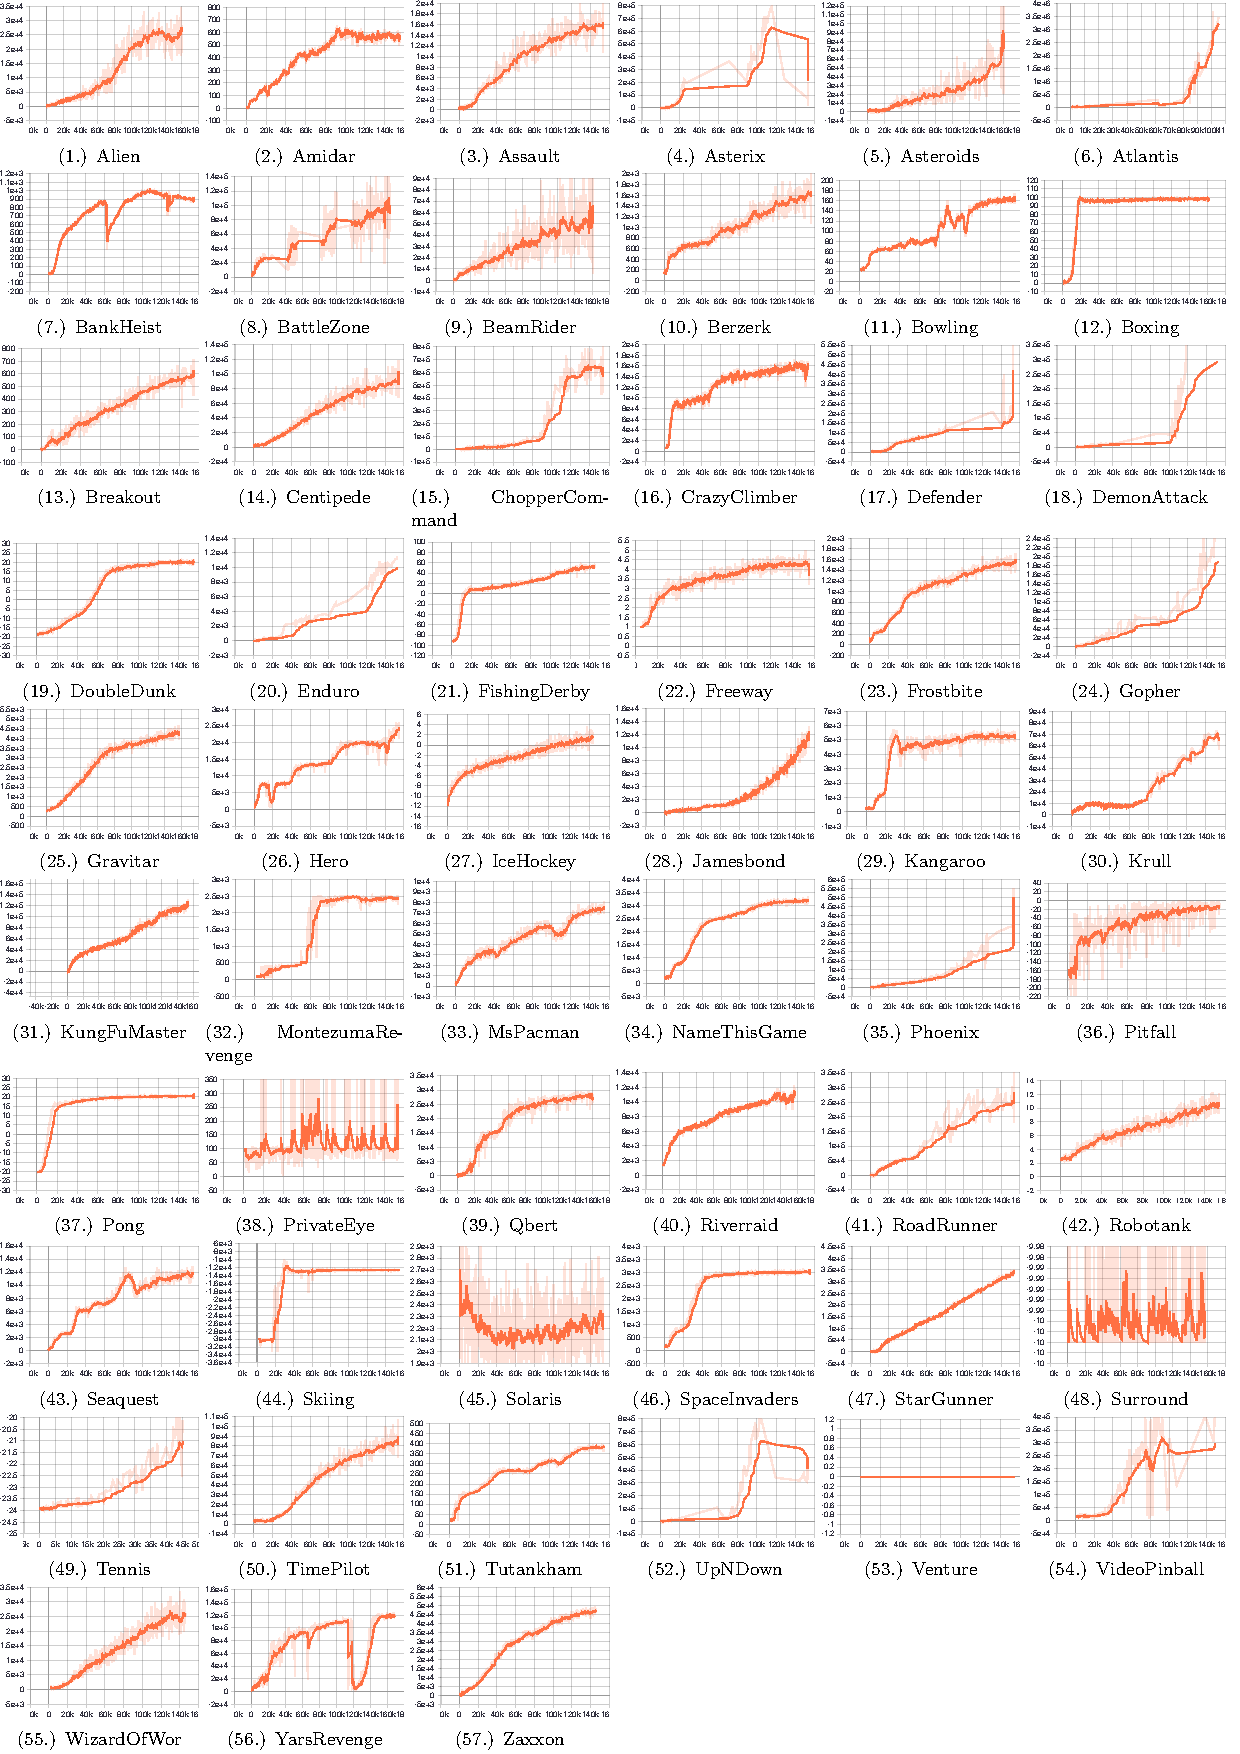
\includegraphics[width=1.0\linewidth]{body/all_fig3.pdf}
\end{figure*}

\clearpage


\onecolumn
\section{Manual analysis}\label{app:man_analysis}

Our quantitative tests provide information on when a model behaves locally and when globally in automated form but they do not consider whether that behaviour is incorrect or not.
More simply put, we do not know whether the changes that we observe are actually resulting in incorrect translations.
We complement these scores with an elaborate manual analysis, which provides more insight into the nature of the non-compositional behaviour we registered.

\subsection{Setup}

\paragraph{Data sampling} We randomly sample 900 examples for substitutivity (100 for each \{model\}$\times$\{test data type\} tuple) and 900 examples for systematicity (50 for each \{model\}$\times$\{test data type\}$\times$\{S$_1^\prime$, S$_3$\} tuple), randomly distributed over templates.
In all cases, we sample sentences randomly from the five seeds that we trained, and from all templates.
For substitutivity, we sample five examples for each synonym for every \{model\}$\times$\{test data type\} pair.

\paragraph{Annotation procedure}
For each of these samples, we annotate how they differ, where we distinguish between four general categories:
\begin{itemize}[noitemsep,topsep=0pt]
\item[i.] \emph{Rephrasing}: part of the sentence is rephrased (but both phrases are equally (in)correct);
\item[ii.] \emph{Source ambiguities}: there is an ambiguity in the source sentence, and the model switches its interpretation; 
\item[iii.] \emph{Errors}: one of the translations contains an error that the other one does not;
\item[iv.] \emph{Formatting}: minor formatting changes, consisting mostly of insertions/deletions of punctuation.
\end{itemize}

\noindent For the substitutivity data, we separately annotate changes that are related to the translation of the synonym, where we distinguish cases in which both synonyms are correctly or incorrectly translated from cases in which one of the translations is correct.
We annotate all changes observed in a sample -- one sentence may thus contain annotations for multiple changes -- and report the relative frequency of each class of errors.

\begin{figure}[h]\centering
\begin{subfigure}[b]{0.25\textwidth}
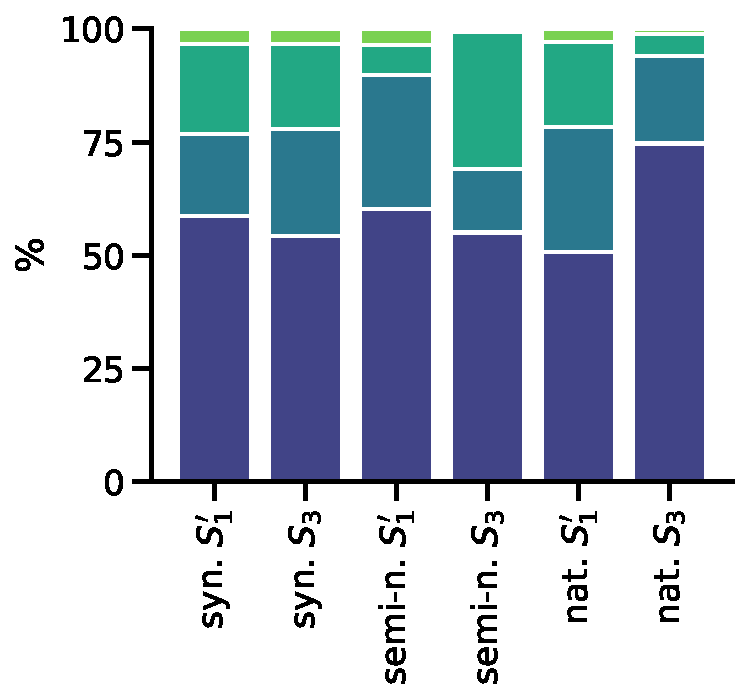
\includegraphics[width=\textwidth]{figures/analysis_appendix/systematicity_small.pdf}
\caption{Small training set}
\end{subfigure}
\begin{subfigure}[b]{0.25\textwidth}
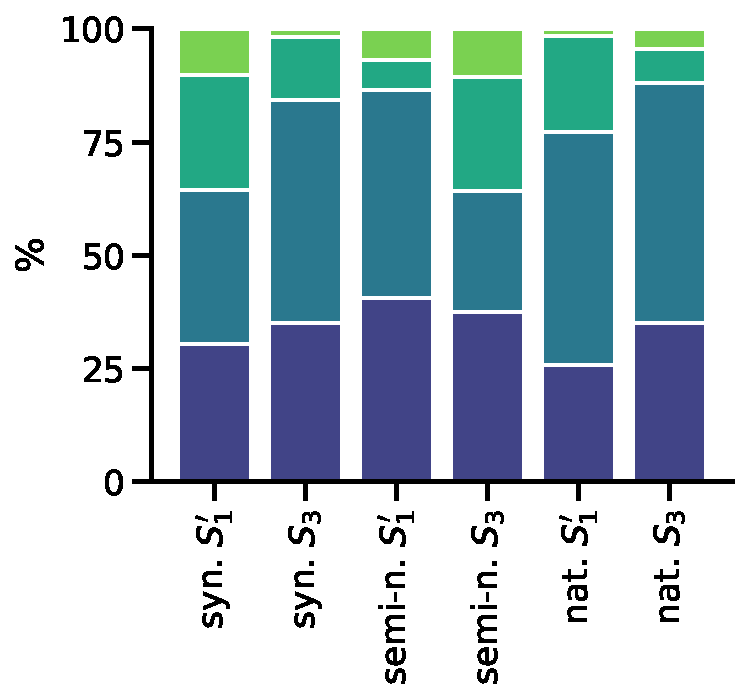
\includegraphics[width=\textwidth]{figures/analysis_appendix/systematicity_medium.pdf}
\caption{Medium training set}
\end{subfigure}
\begin{subfigure}[b]{0.41\textwidth}
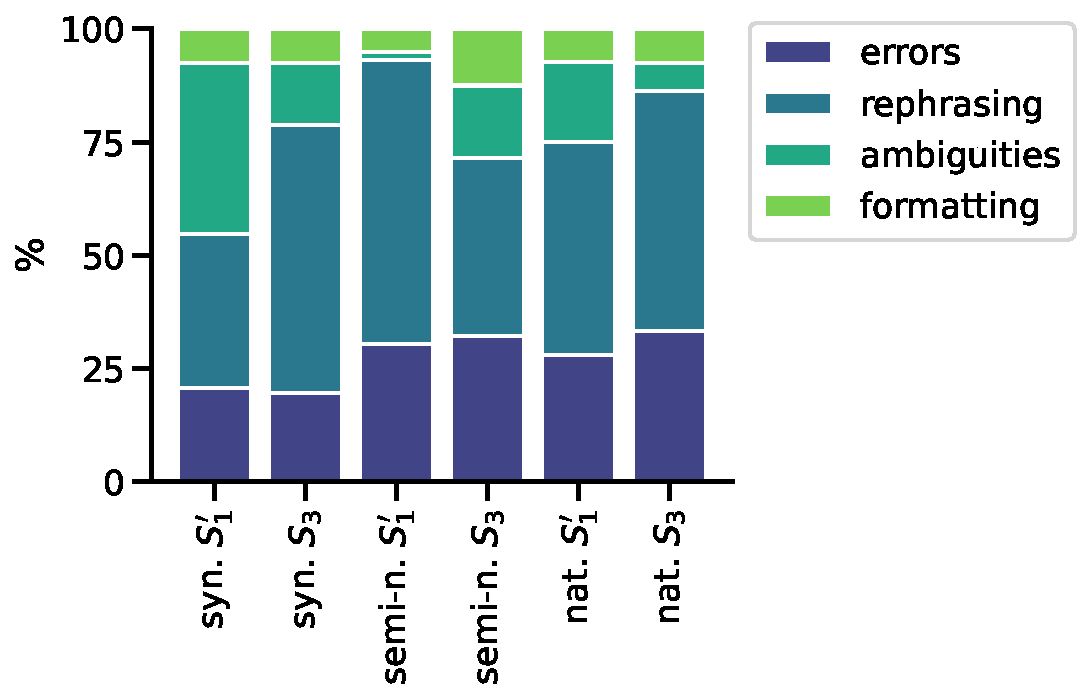
\includegraphics[width=0.9\textwidth]{figures/analysis_appendix/systematicity_full.pdf}
\caption{Full training set}
\end{subfigure}
\caption{Distribution of error types for sentences that contain inconsistencies in systematicity, detailed per model trained on the training set sizes in the subcaptions.}
\label{fig:ap_systematicity_analysis}
\end{figure}
\begin{figure}[t]\centering
\begin{subfigure}[b]{0.22\textwidth}\centering
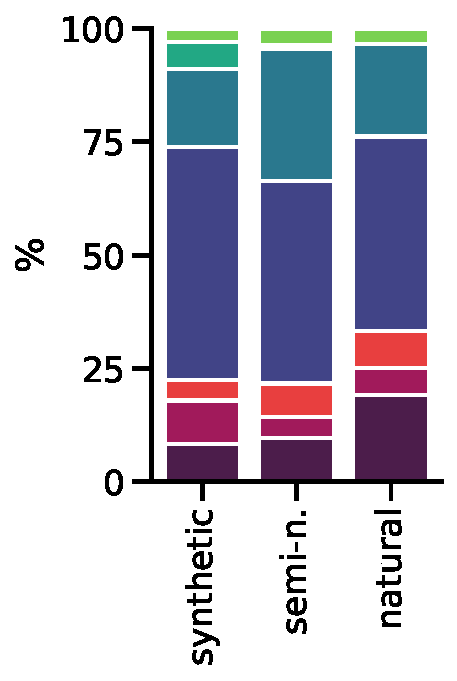
\includegraphics[width=0.79\textwidth]{figures/analysis_appendix/substitutivity_small.pdf}
\caption{Small training set}
\end{subfigure}
\begin{subfigure}[b]{0.22\textwidth}\centering
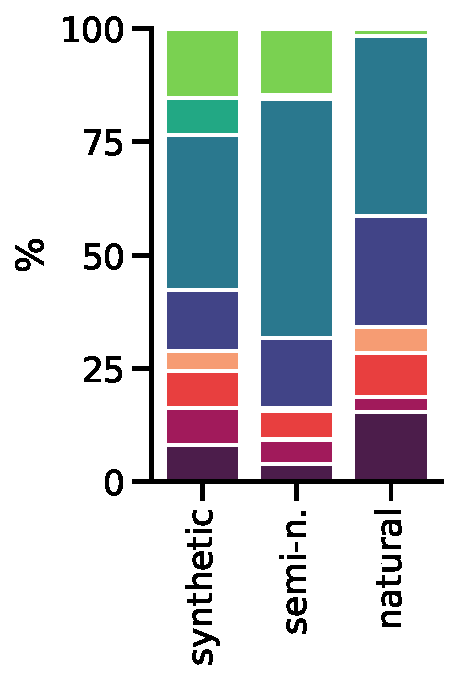
\includegraphics[width=0.79\textwidth]{figures/analysis_appendix/substitutivity_medium.pdf}
\caption{Medium training set}
\end{subfigure}
\begin{subfigure}[b]{0.43\textwidth}\centering
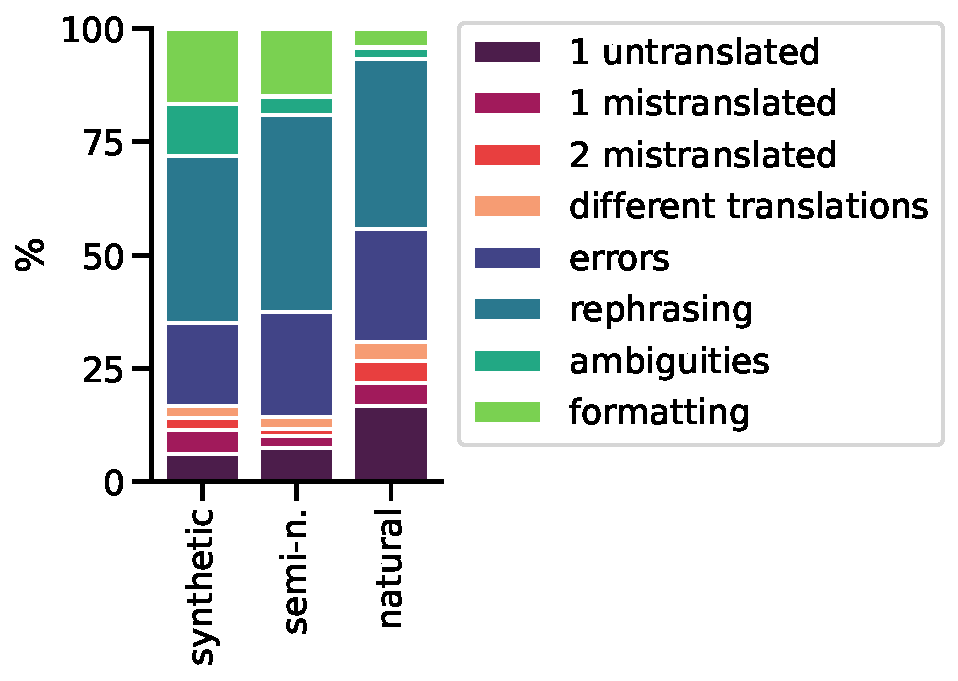
\includegraphics[width=0.85\textwidth]{figures/analysis_appendix/substitutivity_full.pdf}
\caption{Full training set}
\end{subfigure}
\caption{Distribution of the types of inconsistencies observed in the substitutivity test, detailed per model trained on the training set sizes in the subcaptions.
The red colour scheme represents error types specific to this experiment.}
\label{fig:ap_substitutivity_analysis}
\vspace{-.3cm}
\end{figure}

\subsection{Results}

We provide a summary of the results in Figure~\ref{fig:ap_systematicity_analysis} for systematicity and Figure~\ref{fig:ap_substitutivity_analysis} for substitutivity.
As a general trend, the results reflect that in models trained on smaller datasets, more mistakes are actually errors, rather than multiple correct alternatives.
In the systematicity test, 59\% of the inconsistencies for the models trained on the smallest dataset are erroneous changes, versus 34\% and 27\% in the models trained on the medium and largest dataset,
when we average the percentages over the different subsets annotated.
For substitutivity, the percentage of erroneous changes unrelated to the synonyms comprises 46\%, 18\% and 22\% for the smallest, medium and full dataset, respectively.
On top of that, there were inconsistencies related to the synonyms, that represented 26\%, 26\% and 21\% for the three dataset sizes, respectively.
While this is expected, to some extent, it still constitutes a problem: for models trained on smaller amounts of data, being able to translate in a compositional manner is particularly relevant.
Below, we further elaborate on the types of inconsistencies encountered per annotation category, including some examples.

\subsubsection{Rephrasing}
A large portion of the inconsistencies concerns pairs where one translation can be considered a rephrased version of the other translation.
A common cause of this is a \textbf{reordering of words} that does not impact the grammaticality or meaning of the Dutch sentence -- e.g.\ in sentences with adverbs (\exa{heeft de burgemeester zeker in de gaten} vs \exa{heeft zeker de burgemeester in de gaten}) or relative clauses with direct objects (\exa{die genieten van de vakantie} vs \exa{die van de vakantie genieten}).
We could not trace these reorderings back to the specific change made in the systematicity or substitutivity tests.
Consider, for instance, Example \ref{ex:zeker}, where the reordering happens as a consequence of changing the word \exa{king} to \exa{father}.
Note also that while these translations both contain an error (\exa{neemt \dots in de gaten}), this is not marked as an inconsistency, because it is shared between the translations.

\ex.\label{ex:zeker}
\a. \textsc{EN}: The aunts criticise the \{king, father\}, and the man definitely observes the mayor.
\b. \textsc{NL}: (\dots) en de man neemt zeker de burgemeester in de gaten.
\c. \textsc{NL}: (\dots) en de man neemt de burgemeester zeker in de gaten.


Another commonly occurring case of rephrasing is one where the two translations include terms that are (nearly) \textbf{synonymous terms} in Dutch.
Some examples are the translation of athlete (\exa{sporter} vs \exa{atleet}), wish (\exa{wensen} vs \exa{willen}) and observe (\exa{observeren} vs \exa{waarnemen}).
Some of them can appear in the same context but for others the two words would typically appear in different types of texts.
For instance, the word \exa{dokter} is used in more informal contexts than the word \exa{arts} (both translations of \exa{doctor}).
Again, we could not identify an interpretable pattern for when the model emits one instead of the other -- they were not understandably related to the modifications we made to the inputs.

\subsubsection{Source ambiguities}
An intriguing category that we had not anticipated were cases in which the source sentence contained ambiguities, such as \textbf{polysemous words} %whose translation in Dutch is not polysemous 
(e.g.\ \exa{director} translated to \exa{directeur}, referring to the director of a company, and \exa{regisseur}, indicating the director of a movie).
Other ambiguities encountered were \textbf{scope ambiguities}, that were particularly prominent for the systematicity test.
In that test, we concatenate two sentences, and the ambiguity was often related to the verb in the first sentence -- e.g.\ in Example~\ref{ex:director}: 

\ex.\label{ex:director}
\a. \textsc{EN}: The friend wishes that the \{lawyers, directors\} scream, and the victims (\dots)

While we intended this to be a conjunction of two independent sentences, there is also a reading where \exa{wishes} takes scope over the entire second conjunct.
In Dutch, those two cases are distinguishable because they trigger a different word order in the embedded clause (SOV), which is not grammatical for main clauses.
Such scope changes often lead to very questionable interpretations of the English sentence, as is the case for Example~\ref{ex:2CV}:

\ex.\label{ex:2CV}
\a. \textsc{EN}: The victims want that the \{doctors, mayors\} run, and the victims read an article about the case of a procedure which includes a repayment plan.
\b. \textsc{EN}: The farmers think that the \{butchers, mothers\} laugh, and an error can only be seen whenever we have a basic plan that is constantly compared to our real actions.
\c. \textsc{EN}: The women wish that the \{painters, victims\} walk consciously, and every 2CV or Dyane can basically be used as a donor.

Interestingly, the models sometimes also changed the order in the relative clause when a scope change was not possible, for instance when the second conjunct was a question, or the verb in the first sentence did not allow to take scope over the second conjunct without the presence of the word \exa{that}.
See Example~\ref{ex:vaders_president}. We underline the incorrect part of the translation, here and in erroneous examples that follow.

\ex. \label{ex:vaders_president}
\a. \textsc{EN}: The victim observes the \{leader, king\}, and the fathers carefully avoid the president.
\b. \textsc{NL}: Het slachtoffer observeert de leider en de vaders \underline{de president zorgvuldig vermijden}.
\c. \textsc{NL}: Het slachtoffer observeert de koning en de vaders vermijden voorzichtig de president.

These examples indicate that the interpretation of scope change might not be applicable here and that instead, the model is applying some heuristic where particular words trigger a relative clause order.

\subsubsection{Target errors}
In the category `target errors', some of the errors can be easily traced to individual words, whereas others indicate overall misinterpretations of the input.

\paragraph{Single word errors}
Errors that consist of single words are caused by words that are either missing, wrongly translated or untranslated.
Changes due to \textbf{missing words} can be very minor but nevertheless render one of the sentences ungrammatical (e.g.\ \exa{De tante achter de truck bewonderde de directeur}, correct, vs \exa{De tante achter de truck bewonderde directeur}, incorrect),
or yield grammatical sentences that have a slightly different meaning (e.g.\ \exa{de arts die yoghurt eet} vs \exa{de arts die \emph{de} yoghurt eet}).
Missing words can also render translations both ungrammatical and semantically incorrect, which occurred mostly in case of missing nouns or verbs (e.g. \exa{de bakker die ons herkent, merkt de koning op}, correct, vs \exa{de bakker die ons de koning herkent}, incorrect).

We also encountered pairs where one translation contained \textbf{untranslated source words}.
This happened with some of the words in our synthetic templates (e.g. \exa{ooms}/\exa{uncles}, \exa{butchers}/\exa{slagers}) but also with words from the natural sentences (e.g.\ \exa{extrusion}/\exa{extrusie}, \exa{soils}/\exa{bodem}).
These cases mark examples where local processing would have been helpful to the model: as evidenced by the alternative translation in the pair, the model does have access to the correct translation.

Thirdly, we observed cases of \textbf{mistranslated words}, where words unrelated to the change locus received a wrong translation in one of the two sentences but a correct one in the other, for example:
	\exa{poets} being translated as \exa{dichters} (correct) vs \exa{de potten} (incorrect), \exa{general} as \exa{generaal} (correct) vs \exa{wandeling} (incorrect), or \exa{productform} as \exa{productvorm} (correct) vs \exa{productformulier} (incorrect).

\paragraph{Multi-word errors} Other types of errors are less easily located to individual words but indicate an overall misinterpretation of the input, such as the \textbf{change in the tense} as displayed in Example~\ref{ex:musicians},
and the \textbf{change in agreement} displayed in Example~\ref{ex:begrijpen}.
In these particular cases, the source of confusion is explainable: in the first case, the model is combining a present tense verb with a word-order that does not support that, even though such a word order does exist (\exa{in het najaar van 2005 \dots en komen er al snel een paar \dots}).
In the second case, \exa{begrijpen} should agree with \exa{schilder} but instead agrees with the word \exa{doctors}, much earlier in the sentence.
In both of these cases, a more locally compositional approach to translating would have yielded correct translations.

\ex. \label{ex:musicians}
\a. \textsc{EN}: (\dots) and in autumn 2005, five musicians join their forces and soon a couple of potential songs came into being in the rehearsal room.
\b. \textsc{NL}: (\dots) in het najaar van 2005 voegen vijf muzikanten zich bij hun krachten en al snel kwamen er een paar potentiële nummers in de oefenruimte.
\c. \textsc{NL}: (\dots) in het najaar van 2005 bundelen vijf muzikanten hun krachten en al snel \underline{komen} er een paar potentiële nummers tot stand in de oefenruimte.


\ex. \label{ex:begrijpen}
\a. \textsc{EN}: The doctors that laugh admire the \{president, baker\}, the painter that admires her understands the king.
\b. \textsc{NL}: (\dots) de schilder die haar bewondert, \underline{begrijpen} de koning.
\c. \textsc{NL}: (\dots) de schilder die haar bewondert begrijpt de koning.

Finally, we would like to point out an error type that relates to the \textbf{semantic role assigned to agents}, and brings about a lot of other changes in the process.
For instance, in Example~\ref{ex:father}, \exa{the fathers} is removed from the main clause and moved into the relative clause, leaving the main clause without its direct object.

\ex. \label{ex:father}
\a. \textsc{EN}: The group of painters behind the truck forgets the \{president, friend\} and an article about the previous EESC Opinion on alcohol related harm, which looked at f, is read by the fathers
\b. \textsc{NL}: (\dots) en een artikel over het eerdere advies van het EESC over alcoholgerelateerde schade, \underline{die door de vaders wordt onderzocht, wordt gelezen}.
\c. \textsc{NL}: (\dots) en een artikel over het eerdere advies van het EESC over alcoholgerelateerde schade, die naar f uitkeek, wordt door de vaders gelezen.

\subsubsection{Formatting}

We marked inconsistencies as formatting changes if they were related to punctuation, capitalisation, hyphenation or differences in usage of spaces. 
In most cases, those cases were caused by commas: in one translation, a relative clause or two conjuncts were separated by a comma, whereas in the other translation the comma was left out.
In the cases that were caused by spaces (\exa{tumormassa} vs \exa{tumor massa}), there is a slight difference in correctness: in Dutch, compound nouns are not separated by spaces. 
Given how minor these mistakes are, we did not mark them as errors.
Example~\ref{ex:begrijpen} above provides an example for inconsistent usage of commas.
Formatting changes are far from the most frequent but they do become more prominent in models trained on larger training corpora.

\subsubsection{Inconsistencies in synonym translations}

The synonym errors are subdivided into cases where synonyms are simply translated differently (we observed this mostly for the models with larger training set sizes), cases where both translations were incorrect, cases in which only one translation is wrong, and cases in which one synonym was not translated but directly copied from the source.
Sometimes, the changes were quite peculiar, to give some examples from our natural corpus:

\ex.
\a. \textsc{EN}: The child admires the king that eats the \{doughnut, donut\}.
\b. \textsc{NL}: Het kind bewondert de koning die de donut eet.
\c. \textsc{NL}: Het kind bewondert de koning die de \underline{ezel} eet.

\ex.
\a. \textsc{EN}: - Yeah, a barbecue sauce \{moustache, mustache\} contest.
\b. \textsc{NL}: - Ja, een barbecue \underline{[missing `sauce']} met snor.
\c. \textsc{NL}: - Ja, een barbeceu saus snor wedstrijd.

How often each of these errors occur depends on the synonym.
Where some synonyms are more prone to being untranslated (like \exa{ladybird} and \exa{flautist}), some simply received many different correct translations (like \exa{shopping trolley}) yet others received errors very specific to the synonym (like \exa{eggplant} being translated as \exa{egg}$+$\exa{plant}, an interesting case because it reflects processing that is too local).
It should be noted that for all synonyms -- apart from the model with the small training dataset that cannot translate \exa{flautist} and \exa{ladybug} -- we have observed correct translations, indicating that the models did in fact acquire their meaning.

Further, it should be noted that while our substitutivity experiment provides insight into how the model copes with individual synonyms, the majority of the inconsistencies observed were still common target errors, rephrasings, changes in formatting or the result of source-side ambiguities. 
It is vital here to stress that the types of rephrasings, however, did not appear related to the writing style of the sentence. For instance, considering that the synonym changes were related to British and American spelling, and occassionally changed the tone of the sentence (e.g.\ \exa{aeroplane} could be considered more archaic compared to \exa{airplane}), one could anticipate changes in word choice in Dutch reflecting this change of style. However, the inconsistencies were virtually indistinguishable from those annotated for systematicity.
\end{appendices}

\end{document}